\documentclass[letterpaper,11pt]{yalephd}
% remove draft option for final printing.
% font size must be between 10pt-12pt.

%\usepackage{geometry} % you need this for yalephd.cls to work.
%\usepackage{dcolumn}
%\usepackage{amsfonts}
\usepackage{appendix}
%\usepackage{comment}
%\usepackage{cite}
%\usepackage{notoccite}
\usepackage{makecell}

\usepackage[numbers,square]{natbib}
\usepackage{times}
\usepackage{courier}
\usepackage[scaled]{helvet}
\usepackage{url}
\usepackage[utf8]{inputenc} %for utf8 input
\usepackage[T1]{fontenc} %for accented characters
\usepackage{microtype} %better micro typing
\usepackage{datetime}
\usepackage{amssymb} %for shift symbol
\usepackage{amsmath}
\usepackage{mathrsfs} %for mathscr font
\usepackage{listings, multicol, lstcoq} %for code
\usepackage{enumitem}      % adjust spacing in enums
\usepackage{stmaryrd} %for llbracket
\usepackage{mathabx} % for boxes
\usepackage{graphicx} %to include png images
\usepackage{subfig}
\usepackage[usenames,dvipsnames]{color} 
\usepackage{comment}
\usepackage{bussproofs} %for proof trees
\usepackage{flushend}
\usepackage[colorlinks=false,allcolors=black,breaklinks,draft=false]{hyperref} 
\newcommand{\doi}[1]{doi:~\href{http://dx.doi.org/#1}{\Hurl{#1}}} 
\usepackage{mathptmx}      % use Times fonts if available on your TeX system
\usepackage{latexsym}
\usepackage{morefloats}
%\usepackage{bm}
\usepackage{tabu}

\newtheorem{definition}{Definition}
\newtheorem{theorem}{Theorem}
\newtheorem{lemma}{Lemma}
\newtheorem{corollary}{Corollary}
%\newtheorem{invariant}{Invariant}

\usepackage[normalem]{ulem} % for strike out

% please place your own definitions here and don't use \def but
% \newcommand{}{}
\usepackage{prettyref}
\newcommand{\pref}[1]{\prettyref{#1}}
\newcommand{\Pref}[1]{\prettyref{#1} \vpageref[]{#1}}
\newcommand{\ppref}[1]{\vpageref[]{#1}}
\newrefformat{fig}{Figure~\ref{#1}}
\newrefformat{tab}{Table~\ref{#1}}
%----------------------------------------------------

\usepackage{mathpartir}
\usepackage[scaled=0.85]{DejaVuSansMono}
\definecolor{mygreen}{rgb}{0,0.6,0}
\definecolor{mygray}{rgb}{0.5,0.5,0.5}
\definecolor{mymauve}{rgb}{0.58,0,0.82}
\definecolor{ltblue}{rgb}{0,0.4,0.4}
\definecolor{dkblue}{rgb}{0,0.1,0.6}
\definecolor{dkgreen}{rgb}{0,0.35,0}
\definecolor{dkviolet}{rgb}{0.3,0,0.5}
\definecolor{dkred}{rgb}{0.5,0,0}
%----------------------------------------------------

\lstset{ %
	backgroundcolor=\color{white},   % choose the background color; you must add \usepackage{color} or \usepackage{xcolor}
	basicstyle=\ttfamily,      % the size of the fonts that are used for the code
	breakatwhitespace=false,         % sets if automatic breaks should only happen at whitespace
	breaklines=true,                 % sets automatic line breaking
	%captionpos=b,                   % sets the caption-position to bottom
	commentstyle=\color{mygreen},    % comment style
	deletekeywords={...},            % if you want to delete keywords from the given language
	escapeinside={<@}{@>},          % if you want to add LaTeX within your code
	extendedchars=true,              % lets you use non-ASCII characters; for 8-bits encodings only, does not work with UTF-8
	frame=none,	                   % adds a frame around the code
	keepspaces=true,                 % keeps spaces in text, useful for keeping indentation of code (possibly needs columns=flexible)
	keywordstyle=\color{blue},       % keyword style
	language=Octave,                 % the language of the code
	otherkeywords={*, Inductive, Fixpoint, Record, typedef, struct, Function , Definition, Prop, then, true, false, ...},           % if you want to add more keywords to the set
	emph = {in, uint, match, end, with, let, ret, do, forall, exist, :=, =>, ->},
	emphstyle=\bf,%
	moredelim=[is][emphstyle]{|>}{<|},%
	numbers=left,                    % where to put the line-numbers; possible values are (none, left, right)
	numbersep=5pt,                   % how far the line-numbers are from the code
	numberstyle=\scriptsize\color{mygray}, % the style that is used for the line-numbers
	rulecolor=\color{black},         % if not set, the frame-color may be changed on line-breaks within not-black text (e.g. comments (green here))
	showspaces=false,                % show spaces everywhere adding particular underscores; it overrides 'showstringspaces'
	showstringspaces=false,          % underline spaces within strings only
	showtabs=false,                  % show tabs within strings adding particular underscores
	stepnumber=1,                    % the step between two line-numbers. If it's 1, each line will be numbered
	stringstyle=\color{mymauve},     % string literal style
	tabsize=2,	                   % sets default tabsize to 2 spaces
	%title=\lstname                   % show the filename of files included with \lstinputlisting; also try caption instead of title
}

\newenvironment{myproof}{{\bf Proof:}}{\hfill\rule{2mm}{2mm}}

\newif\ifTRthen
\TRthenfalse
\hyphenation{CompCert}
\hyphenation{CompCertX}
\hyphenation{Clight}
\hyphenation{ClightX}
\hyphenation{CertiKOS}
\hyphenation{mCertiKOS}
\hyphenation{mCTOS}
\hyphenation{CTOS}
\hyphenation{mCTOS-hyp}
\hyphenation{mCTOS-rz}
\hyphenation{mCTOS-emb}
\hyphenation{CCTOS}
%% Aonymization
\newif \ifanonymized \anonymizedtrue

\ifanonymized
\newcommand\CTOS{CTOS}
\newcommand\CCTOS{CCTOS}
\else
\newcommand\CTOS{CertiKOS}
\fi
%% END Anonymization

\ifTRthen
\newcommand{\ifTR}[2]{#1}
\else
\newcommand{\ifTR}[2]{#2}
\fi

%\newcommand\mimp{\mathcal{M}_C}
%\newcommand\mabs{\mathcal{M}_A}
\newcommand\mimp{M_C}
\newcommand\mabs{M_A}
\newcommand\layer[3]{(#1,#2,#3)}

\newcommand\pCTOS{p\CTOS}
\newcommand\mCTOS{m\CTOS}
\newcommand\mCTOSbase{\mCTOS{}}
\newcommand\mCTOShyper{\mCTOS{}-hyp}
\newcommand\mCTOSringz{\mCTOS{}-rz}
\newcommand\mCTOSembed{\mCTOS{}-emb}

\newcommand\sem[2]{[\![#2]\!]_{#1}}
\newcommand\join{\!\bowtie\!}
\newcommand\Refrel{\sqsubseteq}
\newcommand\LSem[1]{\textrm{LSem(}#1\textrm{)}}
\newcommand\ClightX[1]{\textrm{ClightX(}#1\textrm{)}}
\newcommand\CompCertX[1]{\textrm{CompCertX(}#1\textrm{)}}
\usepackage{multirow}
\newtheorem{invariant}{Invariant}
\newcommand\ignore[1]{}
\newcommand{\code}[1]{{\it #1}}

\newcommand{\event}[1]{{\mathtt{#1}}}
%\newcommand\oracle{\mathlarger{\varepsilon}}
%\newcommand\oracle{\varepsilon}
%\newcommand\oracle{\mathlarger{\mathlarger{\varepsilon}}}
\newcommand\hardoracle{\oracle_{hs}}
\newcommand\machx{\Pi}
\newcommand\mach[1]{\machx_{\text{#1}}}
\newcommand\machrel{\Refrel}
\newcommand\switch{\!\hookrightarrow\!}
\newcommand{\wbigcup}{\mathop{\widetilde{\bigcup}}\displaylimits}
\newcommand\inv{\texttt{INV}}
\newcommand\set[1]{\{#1\}}
\newcommand\machbe[3]{#1 @ \left(#2, #3\right)}
\newcommand\env[1]{\overline{#1}}
\newcommand\ectxt[1]{{\rm{}EC}({#1})}
\newcommand\ectxtc{{\rm{}EC}}
\newcommand\myscale[1]{\Scale[0.9]{#1}}
\newcommand\push{\mathsf{push}}
\newcommand\pull{\mathsf{pull}}
\newcommand\abst{\mathcal{A}}
\newcommand\primt{\mathcal{P}}
\newcommand{\id}{\textbf{id}}

\newcommand\efrom[1]{(#1\intp)}
\newcommand\eto[1]{(\intp#1)}
\newcommand\ssame{\odot}
\newcommand\sdiff{\triangle}
\newcommand\mysout[1]{\text{\sout{$#1$}}}
%\newcommand\PLayer[3]{#1^{#3}[#2]}
\newcommand\PLayer[3]{#1[#2,#3]}
\newcommand\TLayer[3]{#1[#2][#3]}
\newcommand\Query[3]{#1[{#3}, #2]}
\newcommand\Lthread{L_\comm{thread}}
\newcommand\Lbthread{L_\comm{bthread}}
\newcommand\Lhbthread{L_\comm{hbthread}}
\newcommand\Lhthread{L_\comm{hthread}}
\newcommand{\sstepr}[5]{#1(#2, #3) \ni (#4, #5)}
\newcommand{\sstep}[4]{#1(#2, #3) \ni (#4)}
\newcommand{\para}[1]{\ifTR{}{\vspace{-4pt}}\paragraph{\textbf{#1}}}
\newcommand{\modulef}[1]{#1 \mapsto \kappa_{#1}}

% Useful shorthands used in layer.tex
\newcommand{\pcom}{\parallel}
\usepackage{scalerel}
\DeclareMathOperator*{\bigJoin}{\scalerel*{\Join}{\sum}}
\newcommand{\kw}[1]{{\mathsf{#1}}} % render as a keyword
\newcommand{\pset}[1]{{\mathcal{P}({#1})}}
\newcommand{\Beh}{\mathsf{Beh}} % the set of behaviors
\newcommand{\Ev}{\mathbb{E}} % the set of events
\newcommand{\Prog}{\mathbb{P}} % a set of programs
\newcommand{\Lang}{\mathbb{L}} % a language with log
\newcommand{\Mach}{\mathbb{M}} % a machine
\newcommand{\Env}{\mathcal{E}} % an environment context
\newcommand{\refines}{\sqsubseteq} % refinement relation
\newcommand{\EC}[1]{{\kw{EC}({#1})}} % encironment
\newcommand{\Layer}{\mathcal{L}}
\newcommand{\Rely}{\mathcal{R}}
\newcommand{\Guard}{\mathcal{G}}
\newcommand\oracle{\mathcal{E}}

\newcommand\acq{\mathsf{acq}}
\newcommand\rel{\mathsf{rel}}
\newcommand\deq{\mathsf{deQ}}
\newcommand\enq{\mathsf{enQ}}
\newcommand\reach{\mathsf{reachable}}
\newcommand\now{\mathsf{now}}
\newcommand\ticket{\mathsf{ticket}}
\newcommand{\partf}{\rightharpoonup}
\newcommand\bytelist{\textit{bl}}
\newcommand\spawn{\mathsf{spawn}}
\newcommand\yield{\mathsf{yield}}
\newcommand\cyield{\mathsf{cyield}}
\newcommand\sleep{\mathsf{sleep}}
\newcommand\vundef{\mathsf{vundef}}
\newcommand\ofs{\mathsf{ofs}}
\newcommand\wakeup{\mathsf{wakeup}}
\newcommand\regset{rs}
%\newcommand\tid{\mathsf{tid}}
\newcommand\alist{\rightharpoonup}
\newcommand\tid{t}
\newcommand\eempty{\mathsf{empty}}
\newcommand\option{\mathsf{option}}
\newcommand\qloc{\mathsf{q\_loc}}
\newcommand\perm[1]{\mathsf{status}(#1)}
\newcommand\LAsm{\mathsf{LAsm}}
\newcommand\TAsm{L_\mathsf{pthread}}
\newcommand\boot{\mathsf{x86}}
\newcommand\allid{ID}

\usepackage{xspace}
\newcommand*{\LargerCdot}{\raisebox{0.25ex}{\scalebox{0.7}{$\bullet$}}}
\newcommand\cons{\LargerCdot}
\newcommand\comm[1]{\mathsf{\textcolor{black}{#1}}}
\newcommand\commb[1]{\mathsf{#1}}
%\newcommand\mtext[1]{\mathit{#1}}
\newcommand\replay{\mathbb{R}}
\newcommand\calwait{\mathbb{B}}
\newcommand\any{\cdot}
\newcommand\nonev{\_}
\newcommand\spec{\sigma}
\newcommand\integer{\mathbb{N}}
\newcommand{\PBoot}{L_\mathsf{x86}}
\newcommand{\XAsm}{\mathsf{XAsm}}
\newcommand\CAS{\text{CAS}}
\newcommand\XADD{\text{XADD}}
\newcommand\XCHL{\text{XCHL}}
\newcommand\FAA{\text{FAA}}
\newcommand\FAI{\text{FAI}}
\newcommand\regs{\rho}
\newcommand{\eg}{{e.g.\xspace}}
\newcommand{\ie}{{i.e.\xspace}}
%\newcommand{\cf}{{\em cf. }}
\newcommand{\cf}{see }
\newcommand{\etal}{{\em et al.\xspace}}
\newcommand\step[1]{\overset{#1}{\rightarrow}}
\newcommand\emptye{\epsilon}
\newcommand\model{\models}
\newcommand\opsem[3]{l,ge\model #2 \step{#1} #3}
\newcommand\opsems[3]{l,ge\model #2 \overset{#1}{\rightarrow^*} #3}
\newcommand\partialf{\rightharpoonup}

\newcommand\fevent[1]{\tkfig{\nevent{#1};}}
\newcommand\incticket{\comm{FAI\_t}}
\newcommand\incnow{\comm{inc\_n}}
\newcommand\getnow{\comm{get\_n}}
\newcommand\tshared{\comm{tshared}}
\newcommand\holdlock{\comm{hold}}
\newcommand\lockstatus{\comm{lock\_status}}
\newcommand\true{\mathsf{true}}
\newcommand\false{\mathsf{false}}
\usepackage{relsize}
\newcommand{\ltyp}[4]{#1 \vdash_{#2} #3 : #4}
\newcommand{\lltyp}[5]{#2 \vdash^{#1}_{#3} #4 : #5}
\newcommand{\rulename}[1]{\textsc{\smaller{}#1}}

\newcommand\fatom[1]{#1}
\newcommand\fshare[1]{#1}
\newcommand\fprivate[1]{#1}
\newcommand\fpush[1]{\code{#1}}

%\newcommand{\defeq}{\stackrel{\texttt{def}}{=}}
\newcommand{\defeq}{=}

%% COMMENTS 
\newif \ifcomments \commentstrue

\ifcomments
\newcommand{\zhong}[1]{\textbf{\textcolor{red}{[ #1 --Zhong]}}}
\newcommand{\newman}[1]{\textbf{\textcolor{Orange}{[ #1 -- Newman]}}}
\newcommand{\todo}[1]{\textbf{\textcolor{Orange}{[TODO: #1 ]}}}

% show line numbers
%\usepackage{lineno,xcolor}
% Running line numbers:
%\linenumbers
%\setlength\linenumbersep{5pt}
%\renewcommand\linenumberfont{\normalfont\tiny\sffamily\color{OliveGreen}}


\else
\newcommand{\zhong}[1]{}
\newcommand{\newman}[1]{}
\newcommand{\todo}[1]{}
\fi
%% END COMMENTS

  % all the local macros used in the paper

\bibliographystyle{abbrvunsrt}

\begin{document}

% Need to define title before the abstract.
\title{A Simple Automation Engine for Verifying Complex System Software}
\author{Xiongnan (Newman) Wu}
\advisor{Zhong Shao}
\date{April, 2018} % usually not \today.

% All the stuff at the front of your thesis.
\frontmatter

\begin{abstract}
An operating system (OS) kernel forms the lowest level of any system
software stack. The correctness of the OS kernel is the basis for the
correctness of the entire system. Recent efforts have demonstrated the
feasibility of building formally verified general-purpose kernels, but
the cost of such verification is still prohibitive. Furthermore,
it is unclear how to extend their work to verify the functional
correctness of device drivers, due to the non-local effects of
interrupts. Last not the least,  
complete formal verification of a non-trivial concurrent
OS kernel is widely considered a grand challenge, and
none of these systems have addressed
the issues of concurrency, despite the fact that majority
of OS kernels run on multicore machine nowadays.

This thesis presents a novel compositional framework
for building certified interruptible and concurrent OS kernels with device
drivers. We present formal study of abstraction layers, where
each abstraction layer specifies the precise functionality
of underlying implementation with clear assumptions about its
external context. The framework provides
systematic ways of verifying complex system software like OS kernel,
by specifying, programming, verifying, and composing the abstraction
layers. To support device drivers and interrupts,
we provide a general device model that can be instantiated
with various hardware devices, and a realistic formal model of
interrupts, which can be used to reason about interruptible code. 
For concurrency, we have a novel event based model for representing
shared states,
which allows us to verify each process locally by 
making proper assumptions over other processes, and later
merge all individual proofs together to obtain global properties
across the entire concurrent system.

To demonstrate the effectiveness of our new approach, we have
successfully developed a practical concurrent operating system
kernel in our framework.
The kernel consists of 6,500 lines of C and assembly code, runs on stock
x86 multicore machines, and doubles as a hypervisor and boots multiple instances
of Linux as guest on different CPUs. 
The implementation, modeling, specification, and
  proofs are all done in a unified framework (realized in the Coq
  proof assistant), yet the machine-checkable proofs verify the
  correctness of the assembly code that runs on the actual
  hardware.
To the best of our knowledge, this is the first framework with support
on end-to-end verification of low level OS kernel with device drivers,
interrupts, and fine-grained concurrency, in a unified framework.

\end{abstract}


\maketitle
\makecopyright{2018} % change as needed.
\tableofcontents
\listoffigures % remove this if you have no figures.
\listoftables % remove this if you have no tables.

\chapter{Acknowledgements} % this needs to be before \mainmatter.


% Starts proper arabic numbering of pages and chapters.
\mainmatter

\chapter{Introduction}
While safety-critical software is often designed and tested with extra efforts, testing cannot
prove the absence of bugs. Formal verification, despite known as the only way of building
bug-free software systems, has not been exercised widely in practice due to its complexity and cost.
Verification of a reasonably complex system software is known to be extremely more complex and
costly than the development of the software itself~\cite{klein2009sel4,klein14}.


\section{Challenges in Building Formally Verified System Software}

This dissertation aims to provide a very effective and accessible way of proving practical low-level
system software. To achieve this, we need to tackle several main challenges.

First, complex system software consists of highly interdependent subsystems.
The modular reasoning of each small component locally is non-trivial.
Separation logic is one of the most commonly
used tools to reason about the isolation of data structures in the memory
\cite{appel07:tphols,Tuch:2009}. 
\ignore{
On the other hand, it mixes the main functional
correctness logic with the proof
of memory isolation, thus lacks in modularity and hinders opportunities for automation.
}
As a success story,
the seL4 team \cite{klein2009sel4} has developed the first
formally verified practical microkernel.
This work is impressive in that all the proofs were done
in a modern mechanized proof assistant.
On the other hand, it took them 11 person-years to verify 7,500 lines of
C code, still leaving 1,300 lines of C and 500 lines of assembly code
unverified.


Next, the majority of the traditional verification efforts on proving system software go into proving invariant preservation properties.
For example, about 80\% of the properties proved in seL4 are related
to preserving invariants \cite{klein14}. 
Invariants are known to be very expensive
because we not only need to prove that they are preserved by the local function in consideration,
but also for the whole system, i.e., we need to show that the invariants are preserved at any
moment of the whole system execution and cannot be accidentally broken by any functions
in the system, e.g., through pointer manipulation. Even worse, in practice, we normally do
have functions that temporarily break the invariants. For example, an operation to a data structure
that well preserves the invariants could be implemented with multiple auxiliary functions, where
some of these functions temporarily violate the invariants while some re-establish
the invariants later. Traditional verification approaches
do not have a very effective and systematic way of tackling this challenge.

Furthermore, 
in practical system software, device drivers often form a very large component
of the entire code base; 70\% of the Linux 2.4.1 kernel is
device drivers~\cite{Chou:2001}.
Such drivers are found
to be the major source of crashes~\cite{Chou:2001,Ball:2006,Ganapathi:2006}.
A major challenge in driver verification is the interrupt: a non-local
jump to some driver code, triggered by a device. 
Reasoning about interruptible code is
particularly challenging since every fine-grained processor step
could contain a non-local jump, and, upon return, the machine state
could be substantially changed. Even worse, it is not clear how such
reasoning should be done at the C level, which is completely
interrupt-unaware. Existing work either assumes that interrupts are
turned off inside the kernel~\cite{dscal15,verisoft07} or polls the
interrupts at a few carefully chosen interrupt points~\cite{klein14}.

Last not the least, many system software run on multiple CPUs with
multiple concurrent threads.   
The efficient reasoning of arbitrary concurrent executions among various
interdependent components in a complex low-level system is considered
intractable by some researchers~\cite{vontessin13,peters15,Chong:2016:RNW:3040225}. 

\section{A Compositional Automation Engine} 

In this thesis, we present a compositional, and powerful automation engine for effectively
verifying complex system software. 
We believe that the aforementioned challenges are not directly tied to the verification
of the functional correctness itself, and we think the automation engine should focus solely
on providing
very strong automation support for proving the functional correctness of each system component,
completely separate from the reasoning of aforementioned challenges.
We have developed a strong automation tactical libraries that solely focus on
proving functional correctness, and provide a separate logical framework to handle
memory isolation, invariant preservation, device interrupts, and concurrency.

\paragraph{Memory Isolation}
Instead of letting the main functional correctness proof handle the low-level
isolation at the memory level,  we provide a systematic approach to abstract in-memory
data structures into equivalent logical abstract states where the isolation is guaranteed.
For every in-memory data structure, before we verify the corresponding functions operating
on the data, we first develop a new equivalent machine where the in-memory data is gone but replaced
with a logical abstract state. This new machine provides very basic read/write primitives to this
abstract state, which are implemented by simple getter/setter functions in the original machine.
These two machines, what we call {\it abstraction layers}, are proved to be {\it contextually equivalent},
where any program running on the more abstract machine would have the same behavior when it gets
linked with the memory getter/setter code and  run on the other machine.
At the newer abstraction layer, the read/write primitives are the only way to access the new abstract
states, thus the abstract states are completely isolated from the rest of in-memory data and other
abstract states, and cannot be accessed by other primitives or memory operations.
The actual functions, which are implemented on top of the new abstraction layer
using the new read/write primitives, can be verified
effectively with our automation engine completely at the logical level, and we no longer need to deal with
low-level memory or isolation. Here, a new abstraction layer is developed where the verified
functions are turned into logical primitives with their specifications, and new functions can be
further verified on top of this new abstraction layer.

\paragraph{Invariant Preservation}
As we abstract in-memory data structures into logical abstract states, our system invariants
are also expressed in terms of the abstract states. At every abstraction layer, we separately
prove that all the primitives in this layer satisfy all the invariants in this layer. Given that these
primitives are the only way to access the abstract states, by design, we know that any piece of
code running on this abstract machine model would not break the invariants. 
Different abstract states are isolated, thus by design, primitives operating on one abstract
state would not violate invariants imposed on other abstract states.
Furthermore, each
layer could have different sets of invariants, thus we no longer need to introduce entire system
invariants at once, but introduce them gradually at the most appropriate abstraction level.
For example, when we only have auxiliary list operations that break the list integrity invariants,
we can postpone introducing these invariants until we get to the layer where we have
verified the full functions that gracefully operate on the list preserving the invariants.
The intermediate auxiliary primitives that are no longer needed are removed from the new abstraction
layer to make sure the new invariants are preserved, or to avoid unnecessary invariants proof
even when they do preserve the new invariants added.

\ignore{
To experiment with the effectiveness of our automation engine, 
we have successfully verified a practical single-core
operating system kernel with rich features like virtual
memory, process management, hardware virtualization, {\it etc}.
The proof is achieved semi-automatically with our automation
engine implemented in Coq proof assistant and is detailed
in Chapter \ref{chapter:sequential}.
}

\paragraph{Proof Automation}
As the automation engine guarantees the memory isolation and the invariant
preservation, we can take these as given while we perform the functional
correctness proof. Further more, the main complex functional correctness
reasoning can now be performed on logical abstract states with logical
primitives. Based on this, we have developed a collection of strong
automation tactic libraries that can be used to automate the
proof for varieties of C source programs.

\paragraph{Devices and Interrupts}

In addition to the main challenge brought by the device interrupt,
verification of an interruptible system software with device
drivers also faces the following challenges.

{\em interrupt hardware is not static.} It is configured by
software. In order to verify any interesting device drivers (serial,
disk, {\it etc}.), we first need to model the interrupt controller
devices (e.g., LAPIC~\cite{mps97}, I/O APIC~\cite{ioapicd96}), and
formally verify their drivers. This is important because, if the
interrupt controllers are not initialized properly, it may lead to
undesired interrupt behaviors. Device drivers also interact with
interrupt controllers to mask/unmask particular interrupt lines.
These issues have been overlooked in past work, where 
interrupt controllers are assumed to be properly initialized and
their drivers are correctly implemented~\cite{Alkassar:VSTTE08-225}.

{\em Devices and CPU run in parallel.} Thus, the executions of CPU
instructions and device transitions can interleave arbitrarily. Code
verification on this highly nondeterministic machine can be
challenging since it needs to consider device state transitions, even
when the CPU is executing a set of instructions unrelated to external
devices. Recent
work~\cite{Alkassar:OSVE09,Alkassar:VSTTE08-225,Alkassar:VSTTE2010-71}
tries to address this by enforcing a {\it stability} requirement
that device states only change due to CPU operations. 
%
% Using this assumption, they have proven a reordering
% theory and applied it to postpone the execution of all CPU instructions
% unrelated to the device that is currently being manipulated.  They are then
% able to turn the set of assembly level device operations into
% atomic primitives, which are then lifted to their C level verification
% framework as inline-assembly calls~\cite{Alkassar:VSTTE2010-71}.
% Though the stability assumption suffices for their use case, it is
%
This requirement is, however, 
too strong as devices interacting with 
external environments are not stable: a serial device constantly
receives characters through its port, a network card continuously
transfers packets, an interrupt controller (IC) asynchronously
receives interrupt requests, {\it etc}.

{\em Devices may directly interact with each other.} Existing work
assumes that a device driver monopolizes its underlying device and
devices do not influence each other~\cite{Alkassar:VSTTE08-225}. This
assumption does not hold for many devices in practice. For example,
most devices directly communicate with an interrupt controller by
signaling an interrupt.

{\em Device drivers are written in both assembly and C.}  Existing
device driver verification is either done completely at the assembly
level \cite{Alkassar:VSTTE08-225,duan2013} or the verified properties
are only guaranteed to hold at the C level \cite{Ryzhyk_09,Ryzhyk14}.
For realistic use-cases, proven properties should be 
translated down and then formally linked with
the assembly-level proofs.

% {\em The correctness of device drivers needs to be formally connected
%   to the correctness of the OS kernel in a single proof
%   context.}
%
{\em The correctness results of different components should be
integrated formally.} For example, the correctness proofs of device
drivers and the rest of the system
% , both written in a combination of C and assembly,
need to be formally linked as an integrated system,
before one can deliver formal guarantees on the system as a whole. Not
doing so can introduce semantic gaps among different modules,
% wherein a module makes assumptions contradicting with those of another,
a scenario which introduced actual bugs in previous verification
efforts as reported by Yang and Hawblitzel~\cite{hawblitzel10}. Unfortunately,
this formal linking process was found to be even more challenging than
the correctness proofs of individual modules
themselves~\cite{Alkassar:VSTTE08-225}. 
\ignore{Even OS's with user-level
device drivers can suffer if the correctness proofs of their drivers are not
formally linked with those of the kernel. For example,
if some device driver code triggers a page fault at the user level,
the behavior of the corresponding driver is linked to the behaviors of
the page-fault handlers and address translation mechanism of the kernel.}

Following our mantra, we isolate all the above challenges from our main
functional correctness proof such that we can reuse all the techniques
we have developed above for effective verification of device drivers.
To reason about isolation among concurrent devices and the other parts
of the system, we build up a certified ``virtual'' device hierarchy where
the isolation among different ``devices'' are guaranteed by design.
For effective reasoning of interruptible code, we build a new abstract
interrupt model, built upon a realistic
hardware interrupt model through contextual refinement.
As a result, we have built an effective system that systematically enforces the
isolation among different system modules, which is important
for the scalability of any verification effort and critical for reasoning
about interruptible code. 
\ignore{
We have successfully used these techniques to build the world's first fully verified
interruptible OS kernel with device drivers.
The details are presented in Chapter \ref{chapter:driver}.
}

\paragraph{Reasoning about Concurrent Programs}

In concurrent programs, the accesses to the shared states are protected, either by
locks or via lock-free algorithms. On the other hand, in the developers' mind, these accesses
are considered ``atomic'', and this atomicity needs to be reflected in any good specifications.
When we reason about these concurrent programs, the challenges come from the fact
that we need to consider all possible interleaved executions between the current program
and any unknown potential environment programs and prove that even with all these interleaved
executions, the concurrent accesses can be safely shuffled such that we can view as if
the current program accesses the shared states atomically, and this behavior is observably
equivalent to the original interleaved executions.

Again, following our mantra, we have developed an effective way of representing the states
shared among multiple concurrent programs and expressing the invariants on the current program
and assumptions for other companion concurrent programs. While we continue to abstract private in-memory
states into logical abstract states, the shared states are represented instead as a list of globally
observable I/O events, where actual states can be inferred given the list of events. The operations
on the shared states by the current program are specified as appending corresponding events to the
global external log list. The operations on the shared states by other concurrent programs are encapsulated
into the {\it environmental context}, which specifies the shared state changes by providing a list of events
generated by other concurrent programs, under the current concurrent execution context.
By achieving the proof under all possible environmental context, we could conclude that
the verified property holds for any possible interleaved executions among the concurrent programs.
On the actual verification of functional correctness, we always assume all the accesses to the shared
states are protected, e.g., the lock is already held, such that we no longer need to reason about interleavings
during the code verification. The reasoning of interleaved executions is done as a separate next step,
again at a completely logical level.
This allows us to avoid any complexities coming from the concurrency into our automation engine,
and effectively reuse all the existing
verification techniques to verify each concurrent program, and effectively
combine the reasoning into global properties on the combined concurrent programs.
\ignore{
This line of work is presented in Chapter \ref{chapter:concurrent}.
}

\section{Our Contributions}

This dissertation makes the following new contributions:
\begin{itemize}
\item We present a novel, compositional, and powerful automation engine
for verifying C source code against their specifications. Unlike traditional
verification approaches for verifying C programs mixing the proof of memory isolation
and preservation of invariants into the reasoning of functional correctness,
our automation engine takes the memory isolation and invariants as given, and provide
separate mechanisms to guarantee isolation and prove the invariants.
This allows us to provide very strong automation support focusing solely on
proving the functional correctness.
To show the effectiveness of our approach, using the new tools, we have
successfully constructed a fully verified
practical feature-rich certified OS kernels, which runs
on stock x86 hardware and doubles as a hypervisor and boots a version of Linux as the guest.
We managed to achieve the full specification and verification of the kernel within
2 person-years.

\item We have extended the engine with a novel way of representing
devices and drivers, to effectively reason about system software
with device drivers.
Instead of mixing the device drivers
  with the rest of the system (since they both run on the same
  physical CPU), we treat the device drivers for each device as if
  they were running on a ``logical'' CPU dedicated to that device.
  This novel idea allows us to build up a certified hierarchy of
  extended abstract devices over the raw hardware devices, meanwhile,
  systematically enforcing the isolation among different ``devices''
  and the rest of the kernel.

\item We present a novel abstraction-layer-based approach for
  expressing interrupts, which enables us to build certified
  {\em interruptible} system software with device drivers. Our formalization of
  interrupts includes a realistic hardware interrupt model and an
  abstract model of interrupts which is suitable for reasoning about
  interruptible code. We prove that the two interrupt models are
  contextually equivalent.

\item As a case study, we present, to the best of our knowledge, the first verified
  interruptible OS kernel and device drivers that come with
  machine-checkable proofs.  The implementation, modeling, specification, and
  proofs are all done in a unified framework (realized in the Coq
  proof assistant~\cite{coq}), yet the machine-checkable proofs verify the
  correctness of the assembly code that can run on the actual
  hardware.
  
\item We have further extended our engine with an effective way of representing
shared states accessed by concurrent programs and making assumptions
on other concurrent programs. This allows us to reuse all of the
existing verification techniques to verify concurrent programs, assuming as if
they run sequentially, and move all the reasoning of interleaved executions
to a separate logical reasoning framework.  
Using this technique, we have successfully extended the kernel further
into the first fully verified concurrent OS kernel with fine-grained locking.
  
\end{itemize}

\section{Acknowledgment of the Collaborators}

The work described in this thesis is based on joint work with various members
in the CertiKOS project.\footnote{http://flint.cs.yale.edu/certikos/}
The author is one of the two critical contributors for developing the methodology
on performing large-scale verification by building stacks of certified abstraction layers
using two common patterns, presented in Chapter \ref{chapter:framework}. The automation
engine for proving the C source programs (described in Chapter \ref{chapter:automation})
are developed solely by the author, which is particularly suitable for the
layer-based methodology and is the critical component of the framework. 
The author is also one of the two main contributors of the verified kernel (presented
in Chapter \ref{chapter:sequential}), and the
extension to the framework to reason about device drivers and interrupts
(detailed in Chapter \ref{chapter:driver}), and a critical contributor
of the log-based approach on reasoning
concurrent programs (illustrated in Chapter \ref{chapter:concurrent}). 


        % Introduction 

\chapter{Certified Abstraction Layers}
\label{chapter:framework}


In this section, we give a detailed overview of our abstraction-layer-based
approach on verifying system software. The exact techniques are used
in the verification of the mCertiKOS kernel presented in chapter \ref{chapter:sequential}.
As in any other system verification, we associate every code module (a piece of code,
or normally, a function)
a specification, and prove that the code meets its specification, or more
formally, there is a {\em forward simulation}~\cite{Lynch95} from the module
implementation to its specification. A specification of a module is a logical
abstract representation of the module's behavior with the concrete
implementation details hidden. We expect the verification to be compositional,
i.e, when we reason about other code modules that utilizes existing verified
module $M$ (e.g., it calls a function in $M$), we expect the verification
of the new modules only looks at the specifications of $M$, given the fact
that $M$ is already proven to meet its specification, so that the verification
never needs to look into the actual implementation of $M$. At the moment $M$ is
being verified, you may not know how $M$ will be used later or what properties of
$M$ may be useful for any global properties you may get interested in.
Thus, we insist the specification of $M$ always capture everything
we may want to know about it. We call such specification a {\em deep specification}.
More formally, for any deep specification $s$, any two implementations that satisfy $s$
should have contextually equivalent observable behaviors. 

When we write a specification for a module, we normally hide the
concrete private data representation in the memory, to ensure the client
of the module can only access the data through defined public interfaces
and thus cannot possibly break any invariants imposed on the private
state in the module implementation. However, in the case of deep
specification, in order to capture any potential behaviors in the
specification itself, we also need to introduce an abstract state
in substitute the concrete private data to use it to specify
full functionality of each public interface of the module.

For example, to specify operations on a doubly
linked list stored in memory, we may logically interpret the complex in-memory
data structure as a simple logical list and specify its {\em push} and {\em pop}
operations as a simple list {\em append} and {\em remove} operations. To support
this, the framework needs to provide a systematic way to hide the private memory
state from its client, and replace them with {\em abstract states} to specify
the full functionality of each operation in the interface in terms of the {\em
abstract states}. It also needs to make sure that this transformation is
sound, i.e., any client code using the {\em push} and {\em pop} operations
on a list should have exactly same behaviors when it is reasoned using the
abstract local specifications and using the concrete doubly linked list
implementation.

\ignore{
Furthermore, a complex system like a kernel module is normally
implemented in a combination of the C and assembly language. Thus, the framework
should be able to be instantiated in both languages and provide a way to
certifiably compile the C-based framework into the assembly-based one. The {\em
certified abstraction layers} provide exactly such support.
}


To better illustrate how the certified abstraction layers work,
in this chapter, we use the verification of a console
circular buffer implementation used in our verified device drivers
as a running example. We show the details step by step and introduce
the concept and definitions used in the verification as they appear.
Fig.~\ref{fig:source:cons-buf} shows the implementation of the circular
buffer in C. The buffer is represented as a circular array
(to store the received input characters) with two additional
fields. The field \texttt{rpos} represents the head of the buffer,
i.e., the index of the next character to read, while the field
\texttt{wpos} indicates the index of the array where the next character
should be written to. When both fields collide, i.e., when both
indexes are the same, it means the buffer is empty. This is why we need
to allocate one extra space (line 2) in order to store \textsf{CB\_SIZE}
characters in the buffer, in which case, the \textsf{wpos} would be
``one index less'' than \textsf{rpos}. 
The figure also defines three functions
\textsf{cb\_init}, \textsf{cb\_read}, and \textsf{cb\_write} that operate
on the circular buffer. The function \textsf{cb\_init} clears the buffer
by setting both \textsf{rpos} and \textsf{wpos} to zero. Note that
it actually suffices to set them arbitrary same value. The function
\textsf{cb\_read} reads a character from the buffer and updates the
indexes accordingly, returning a special character \textsf{CB\_EMPTY}
when the buffer is empty (when the indexes have the same values);
while \textsf{cb\_write} writes a character to the buffer, chopping
off the head character if the buffer was full.

To write a deep specification for the circular buffer, we can use a logical
abstract integer list to represent the in-memory circular buffer implementation.
Then the three operations in Fig.~\ref{fig:source:cons-buf} can be
abstractly specified as they are shown in Fig.~\ref{fig:spec:abs-cons-buf}
using the abstract list as its private data. Here, we use the
notations $[\cdot]$ and $\textsf{++}$ to represent a singleton list and list
concatenation, respectively. The specification shown in
Fig.~\ref{fig:spec:abs-cons-buf} is much cleaner and simpler than the actual
implementation which simplifies future reasoning of code modules that use the
data structure.

\begin{figure}
\lstinputlisting [language = C, multicols=2] {src/console.c}
\caption{Console circular buffer implementation}
\label{fig:source:cons-buf}
\end{figure}

\begin{figure}
\[
\begin{array}{cr}
\inferrule{
}{
	\mathsf{cb\_init} (cb) \defeq \mathsf{nil}
} & \text{(cb\_init)} \\ [5ex]

\inferrule{
	c :: tl = cb \\
}{
	\mathsf{cb\_read} (cb) \defeq (tl, c)
} & \text{(cb\_read\_char)} \\ [3ex]

\inferrule{
	\mathsf{nil} = cb 
}{
	\mathsf{cb\_read} (cb) \defeq (cb, CB\_EMPTY)
} & \text{(cb\_read\_empty)} \\ [5ex]

\inferrule{
	\mathsf{length}~cb < CB\_SIZE \\
}{
	\mathsf{cb\_write} (cb, c) \defeq cb \textsf{++} [c]
} & \text{(cb\_write\_char)} \\ [3ex]

\inferrule{
	h :: tl = cb \\
	\mathsf{length}~cb = CB\_SIZE \\
}{
	\mathsf{cb\_write} (cb, c) \defeq tl~\textsf{++}~[c]
} & \text{(cb\_write\_overflow)} \\
\end{array}
\]
\caption{Specifications of abstract console buffer primitives}
\label{fig:spec:abs-cons-buf}
\end{figure}

Next, we show how we can prove the abstract deep specification
is equivalent to the actual C implementation in arbitrary client context.
We first show how we represent the abstract states and primitives
in our framework.
Then we show the source language our code module is implemented in,
how we reason about the source code written in the language utilizing
the abstract states and primitives,
and how we link everything to reach the final
{\em contextual refinement} property we seek for.

In this chapter and the following chapters, I try my best to present the exact
implementations of example definitions, specifications, and proofs
directly in Coq, instead of in an invented logical notations
(like derivation rules in Fig.~\ref{fig:spec:abs-cons-buf}).
The purpose is to help the readers to better understand how the certified
abstraction layers are implemented in Coq in our framework, instead of
merely getting the high level ideas. The hope is to make it easier for others to
reproduce our work for their own purpose.


\section{Layer Interface}
\label{sec:layer_interface}
To support the deep specification, the framework needs a formal notion
that can be used to represent an arbitrary list of abstract states,
and a set of abstract primitives that operate on the abstract states. 
Furthermore, the framework should be able to enforce a set of system
invariants on the abstract states which gets preserved across
the system execution, especially by the abstract primitives.
A {\em layer interface} serves such a purpose.

A layer interface $L$ consists of the {\em abstract states}, {\em
  primitives}, a set of {\em invariants} on the abstract states, and
{\em proofs} that all the primitives in the layer interface preserves
the layer invariants.  An {\em abstract state} could be a logical
state that does not correspond to any physical state in the machine,
but in most cases, it is a logical state that is abstracted from a
concrete state in the registers or memory. Each {\em primitive}
operates (exclusively) on the abstract states and is associated with an atomic
specification. It is abstracted from a concrete, verified piece of the
actual code.  

\begin{figure}
\lstinputlisting [language = Coq] {src/cons_buf_spec.v}
\caption{Specifications of abstract console buffer in Coq}
\label{fig:cons_buf_spec}
\end{figure}

As an example, we show how we implement a layer interface in Coq
for the abstract console buffer shown in Fig.~\ref{fig:source:cons-buf}
and \ref{fig:spec:abs-cons-buf}. Fig.~\ref{fig:cons_buf_spec} shows
our actual Coq implementation. First, the type of abstract states
is always defined as a Coq \textsf{Record} with each record field
representing concrete abstract state.
As explained before, the abstract console buffer (named \textsf{cb})
is represented as a Coq list of integers (line 1-4).
Line 6 to 20 shows the specifications of three abstract primitives
in Coq. Here, $cb~d$ represents retrieving the field $cb$ from the
abstract state $d$, and $d~\{cb: newcb\}$ indicates a new abstract state
$d'$ with the field $cb$ equal to the provided new value $newcb$ and
otherwise the same as $d$. The specifications shown in Fig.~\ref{fig:cons_buf_spec}
are the Coq implementations of the ones presented in Fig.~\ref{fig:spec:abs-cons-buf}.

Furthermore, we also define an invariant over the abstract buffer
in this layer interface.

\begin{invariant}[valid console buffer length]
\begin{align*}
0 \leq \textsf{Zlength} (d.cb) \leq \textsf{CB\_SIZE}
\end{align*}
\end{invariant}

The invariant says that the length of abstract buffer should always
be between zero and the given maximum size.
It is not hard to prove that all of the three primitives preserves
this invariant.

Given the layer interface, we need a way to incorporate the layer interface
into our source language so that the code implemented in the source language
can utilize the primitives to manipulate the abstract states, while always
maintaining the data invariants. Our framework support both a C-like
language ClightX (which is an extension to the CompCert Clight language
with our layer interface) and an x86-based assembly language LAsm
(which is an extension to the CompCert Asm language for the x86
architecture with layer interface). In the subsequent sections,
we first define these two languages formally, then present
a formal notion of {\em certified abstraction layers} that can be used
to verify the mode modules with deep specifications.

\ignore{
Since the {\em invariants} are preserved by all the
primitives, the abstract states can only be accessed through calling
one of the primitives, and execution of the primitives are atomic, the
invariants hold at any moment during the system execution.
}


\section{Language ClightX}

\begin{figure}
\lstinputlisting [language = Coq] {src/clight_expr.v}
\caption{Clight expressions}
\label{fig:clight_expr}
\end{figure}

\begin{figure}
\lstinputlisting [language = Coq] {src/clight_stmt.v}
\caption{Clight statements}
\label{fig:clight_stmt}
\end{figure}

In this section, we introduce the language ClightX, which is the C-like
language our framework supports. 
The language ClightX is an extension of the language Clight~\cite{blazy-leroy-clight}
supporting the layer interfaces. We first present the language Clight in detail.

Language Clight is a subset of C and is
formalized in Coq as part of the CompCert project~\cite{compcert}.  Its formal
semantics relies on a memory model~\cite{leroy08} that is not only
realistic enough to specify C pointer operations, but also designed to
simplify reasoning about non-aliasing of different variables.
From the programmer's point of view, 
Clight avoids most pitfalls and peculiarities of C such
as nondeterminism in expressions with side effects. 
On the other hand,
Clight allows for pointer arithmetic and is a true subset of C: valid
Clight programs are valid C programs with the same semantics.
Such simplicity and practicality turn Clight into a solid choice for
certified programming.
Furthermore, the CompCert verified compiler
provides strong guarantees on code
obtained by compilation of Clight programs.

\subsection{Syntax of Clight}

Fig.~\ref{fig:clight_expr} and Fig.~\ref{fig:clight_stmt} shows the formal
definitions of Clight expressions and statements in Coq, respectively.
With the help of comments, the figures should be self-explanatory.

Note that Clight expression is free of side effects. Thus, a function
in Clight cannot be an expression, as executing the function body
may trigger side effects, e.g., it may change the system state like the memory.
Instead, as shown in the figure, a function call is a statement in Clight,
and in order to support the assignment of the form $v = f(a_1, \cdots, a_n)$, the
statement \textsf{Scall} takes an optional variable identifier as the first  argument,
which represents the variable we would like to write the return value to.
It is optional because the function may not have any return value, or the return
value may get discarded instead of getting written to a variable, i.e.,
it maybe simply of the form $f(a_1, \cdots, a_n)$ in the standard C format.

Furthermore, Clight only defines an infinite loop
(line 10 in Fig.~\ref{fig:clight_stmt}), and the common C loop constructors
like \textsf{while}, \textsf{do while}, and \textsf{for} loops are defined
separately in terms of the infinite loop \textsf{Sloop} (line 25-32
in Fig.~\ref{fig:clight_stmt}). 
In our verified code, we never use
the \textsf{goto} statement.
The language also supports special set of functions built into the language.
They are not used in our framework, and thus are omitted from Fig.~\ref{fig:clight_stmt}.

\subsection{Semantics of Clight}

Next, we present the formal semantics of Clight. CompCert defines
both a small-step and a big-step semantics for Clight, which are proven
to be equivalent. In this subsection,
we only present the big-step semantics, as it is simple and our automated
verification tactics is designed based on it.

\paragraph{Clight States}
Clight states consist of following components.
\begin{itemize}[leftmargin=*]

\item Memory state \textsf{m} of type \textsf{mem} is the main memory
that uses the CompCert memory model. Instead of viewing the main memory
as a huge consecutive sequence, the memory is represented as a list of
disjoint CompCert memory blocks. A pointer to the memory is represented
by a block id and an offset within the block (offsets starts from zero).
Each block has its own size and it is not allowed to go beyond the block boundary
or move to another block through any pointer arithmetic operations.
Full details can be found in ~\cite{leroy08}.  

\item Global environment \textsf{ge} of type \textsf{genv} represents the mapping
from global variable/function identifiers to the memory blocks that the variables/functions
are stored. Since CompCert memory stores each global variable and function into
its own memory block, storing the offset is not necessary (it is always zero).
This mapping is fixed once the system code is fixed and can be constructed
before the system executes the main function. Thus, during the execution, 
this mapping never changes.

\item Local variable environment \textsf{e} of type \textsf{env} gives the
mapping from the local variable identifiers to their memory locations
(memory block and offset). Note that since more than one local variables
could be on the same memory block (e.g., on the same stack), the mapping
in this case also gives the block offset. This mapping also does not change
during the system execution since no variable locations vary during the system
execution, though their values stored in those locations may change during the
execution.

\item Local temporary environment \textsf{le} of type \textsf{temp\_env} is
a mapping from local temporary variables to their actual values. Temporary
variables are special variables in Clight designed for optimization and
they are not stored in memory (similar to the register variables in GCC).
When we generate the Clight code, we can scan the code and find
all the variables that are never taken address of, and represent
them using the temporary variables
instead of the above local variables. Given that they are never taken the
address of, it is not necessary to store them in the memory, and we just need
to keep the logical mapping from their identifiers to their actual values.
The compiler optimization can then save them in the registers instead of memory
if possible. Note that since the mapping saves the actual values of the temporaries,
\textsf{le} changes during the system execution.


\end{itemize}


\paragraph{Expression Evaluation}
Fig.~\ref{fig:clight_eval_expr} shows the rules for evaluating Clight
expressions. The definition is parameterized over the memory $m$,
global environment $ge$, variable environment $e$, and the temporary
environment $le$. Note that Clight expressions do not produce any
side effects. That means evaluating Clight expressions does not
change any of the above system states.
As shown in Fig.~\ref{fig:clight_eval_expr}, the rules are defined inductively
with each constructor corresponds to some expression shown in Fig.~\ref{fig:clight_expr}.
The inductive definitions for evaluating right and left values are defined
mutually recursively.

\paragraph{Statement Execution}
Fig.~\ref{fig:clight_exec_stmt} and Fig.~\ref{fig:clight_exec_stmt2}
shows the big-step semantics on executing the Clight statements.
The inductively defined predicate \textsf{exec\_stmt} takes
the Clight states and a Clight statement, and produces
an event trace, a new temporary environment and memory, and
an execution outcome. Here, the event trace \textsf{t} of type
\textsf{trace} is used to represent the list
of external observable events. It is not used in our verified system, thus
the value of trace \textsf{t} is always the empty trace \textsf{E0}.
The execution outcome \textsf{out} of type \textsf{outcome} indicates how
the execution terminated, either normally (\textsf{Out\_normal}), or prematurely
through a break (\textsf{Out\_break}) or a continue (\textsf{Out\_continue})
statement. The value \textsf{Out\_return} of type $option~(val * type)$ is used to indicate
the termination by returning a value of given type, or \textsf{None} if
just by returning with no return value.

Fig.~\ref{fig:clight_exec_stmt} shows the semantic constructors for a subset
of Clight statements. The majority of the rules in the figure should be
self-explanatory. Note that there are two rules for the sequential compositions
(line 15-22), where the first rule (line 15-18) represents the case when
both composed statements executes sequentially (the first statement terminates
with \textsf{Out\_normal}), while the second rule (line 19-22) explains
the case when the execution of first rule stops abnormally and the whole sequence
terminates without executing the second statement.

Fig.~\ref{fig:clight_exec_stmt2} presents the semantic rules for more
complex statements, i.e., loops and function calls.
The various predicates related to the execution outcome is defined in
Fig.~\ref{fig:clight_outcomes}.

Recall that Clight defines only one native loop constructor called \textsf{Sloop},
where the common loop definitions are derived from \textsf{Sloop}.
As shown in the figure, there are three execution rules for the loop $\textsf{Sloop}~s1~s2$.
The main rule \textsf{exec\_Sloop\_loop} (line 14-19) represents the case
when both $s1$ and $s2$ terminates normally and the loop gets into the next iteration.
It first executes the first statement $s1$ (line 15) that terminates normally (line 16),
then it runs the second statement $s2$ (line 17), and continues the next iteration (line 17).
Note that the termination due to the \textsf{continue} statement is also
considered normal (line 16), since \textsf{continue} simply means not to execute
the subsequent statements in the loop body, but does not mean to terminate the loop.
The other two rules for the loops are the cases when the loop terminates.
The rule \textsf{exec\_Sloop\_stop1} represents the case when running the first statement
(line 5) terminates abnormally through the \textsf{break} or \textsf{return} statements
(line 6), in which case it terminates the entire loop.
The second rule \textsf{exec\_Sloop\_stop2} shows the case when running the first
statement (line 9) terminates normally (line 10), but the execution of the second
statement (line 11) stops abnormally (line 12), which again causes the entire execution
to jump out of the loop.

There is a single rule for executing a function call statement
$\textsf{Scall}~optid~a~al$.
Understanding this rule is critical in getting the idea on how we extend the
Clight language with the layer interfaces. As shown in
Fig.~\ref{fig:clight_exec_stmt2}, it first checks whether the type
of the function expression is valid, i.e., whether the type of $a$ is
either a function or a function pointer (line 21).
Then the function expression $a$ is evaluated (line 22), followed
by the evaluation of the argument list $al$ (line 23). After some sanity checks
(line 24 and 25), the function is evaluated with the argument values
(line 26) and the result is written to the optional variable in the $optid$
if necessary (the \textsf{set\_opttemp} part in line 27).
The predicate \textsf{eval\_funcall} that actually evaluates the function
is defined mutually recursively below in the figure. 
As shown in the figure, there are two kinds of functions in Clight.
One is the internal function that is implemented within the module,
which is evaluated by executing the function body recursively using
the \textsf{exec\_stmt} predicate above (line 32), and the other
is called external functions used to represent the functions from
some external sources that get linked with the current module.
Clight requires every external function to provide the semantics on
how the call changes the system states, which is encapsulated in
the \textsf{external\_call} predicate (line 35). It also requires
the proof that the semantics satisfies a list of predefined properties
to respect the compiler correctness.

\begin{figure}
\lstinputlisting [language = Coq] {src/clight_eval_expr.v}
\caption{Evaluation rules for Clight expressions}
\label{fig:clight_eval_expr}
\end{figure}

\begin{figure}
\lstinputlisting [language = Coq] {src/clight_exec_stmt.v}
\caption{Big-step semantics for Clight: part 1}
\label{fig:clight_exec_stmt}
\end{figure}

\begin{figure}
\lstinputlisting [language = Coq] {src/clight_exec_stmt2.v}
\caption{Big-step semantics for Clight: part 2}
\label{fig:clight_exec_stmt2}
\end{figure}

\begin{figure}
\lstinputlisting [language = Coq] {src/clight_outcomes.v}
\caption{Outcomes of statement execution}
\label{fig:clight_outcomes}
\end{figure}


\subsection{Extending Clight to ClightX}

The key idea behind deep specification and the layer-based approach
is to gradually abstract the in-memory private data into simpler logical
abstract states and the functions manipulating the private data
into logical atomic primitives operating on the abstract states instead.
Thus, we need a way to extend Clight so that the language can be instantiated
with different layer interfaces. In other words, the language ClightX
needs to be parametric over a layer interface $L$. 
The standard Clight semantics is unaware of either the
abstract states or the abstract primitives defined in the layer
interface. Therefore, there are two challenges
in this extension. First, the state of Clight language should be extended
to support the abstract states. Second, we also need to support
the abstract primitives so that we can syntactically invoke these primitives
in the ClightX source code and the semantics of these primitive calls
should not only change the old system states in Clight, but especially it
should be able to update the abstract states as well.

On the other hand, we seek to minimize the impact on the existing proof
infrastructure for program and compiler verification. Thus, we do not
modify the semantics of basic operations of Clight, but access the
abstract states exclusively through the Clight's external function
mechanism provided in Clight. Recall that
Clight axiomatizes the behaviors of external functions without
specifying them, and only assumes they do not behave in a manner that
violates compiler correctness. We use the external function mechanism
to extend Clight with our primitive operations, and supply their
specifications to make the semantics of external functions precise. 
The remaining challenge is that, as shown in the line 37 of
Fig.~\ref{fig:clight_exec_stmt2}, the type of external function semantics
are already fixed by Clight and it does not contain the new abstract states
as mutable states in the type. Fortunately, the memory model used in
the Clight semantics is an axiomatized memory model, which does not
give any concrete implementation, for example, on the concrete type
of the memory. Thus, we instrument original memory type $mem$ as a
new pair $mem * RData$, and instrument the memory access operation
to access the first part of this new pair. This allows us not to change
any of the old Clight semantics for the old operations of Clight,
while still be able to give semantics to the external functions (primitives)
that changes the abstract state part (the second element in the pair)
of the new memory type.

As a result, the language ClightX is parametric over the layer interface,
or more specifically, the type of abstract states $RData$ (as the second
element in the memory pair), and the list of abstract primitives (as the
list of available external functions) specified using the memory pair
(the memory and the abstract states).

The specification of external functions in ClightX (shown in line 37 of
Fig.~\ref{fig:clight_exec_stmt2}) is defined as an inductive predicate,
and operates on both the memory and abstract states (thanks to the parameterization
of the memory as a pair). On the other hand, the semantics of ClightX is
deterministic given a layer interface. Furthermore, in majority of the
cases, the primitive in the layer interface does not change the main memory.
This is because, we always try to first abstract the memory into logical
abstract states and specify the primitives in terms of the abstract
states. Thus, in our framework, the specifications of primitives
are mostly written as a Coq function, as they were shown in Fig.~\ref{fig:cons_buf_spec}.
We have implemented a simple transformer that converts the functional form
into predicates when they are passed to ClightX. The functional form
is more concise and readable. Another benefit is that we do not need to
prove each primitive specification satisfies the external call properties
defined in CompCert. They are proved once and for all in the transformer.

\subsection{Code Module in ClightX}

Given the definition of the language ClightX above,
we can implement the code modules, e.g., the console buffer
implementation shown in Fig.~\ref{fig:source:cons-buf}, in ClightX
and formally reason about their properties using the formal semantics
of ClightX. On the other hand, the ClightX syntax is defined
in the abstract syntax form, which is very inconvenient
to write comparing to the standard C format. Instead,
our ClightX code is automatically generated from standard C code
through a tool called $\textsf{clightgen}$ provided by CompCert~\cite{compcert}.
We directly verify the generated ClightX code. Thus, correctness
of the $\textsf{clightgen}$ does not affect the correctness of
the verified code.

For simplicity, in the examples used throughout the thesis, we show
the source code directly in the standard C, even though in Coq, they
are implemented in ClightX.


\section{Language LAsm}
Even though majority of the system software is implement in C,
we would like our formal claim to be made at the actual compiled assembly
code running on the machine. Furthermore, many of the system software
has some snippet of code directly implemented in assembly.
Thus, we need a formal notion of an assembly language with
the support of parametric layer interface.

\subsection{Syntax and Semantics of LAsm}

The language LAsm is a super set of the CompCert x86 assembly language with more
machine-dependent registers and instructions needed for implementing
low level system software. 
Fig.~\ref{fig:lasm_regs} shows the register definitions in LAsm.
They are mostly consistent with the standard x86 assembly language,
except the special pseudo register $RA$ representing the return
address (line 26). In x86, the return address is normally stored
on the stack when a function is called, but in LAsm (also in
CompCert assembly) it is saved in this special pseudo register $RA$.
It is called a pseudo register because it does not really exist
in a physical machine. 

Fig.~\ref{fig:lasm_instructions} presents a small subset of assembly
instructions in LAsm, with their small-step formal semantics
detailed in Fig.~\ref{fig:lasm_semantics}.
The statements and their semantics are
mostly similar to the standard x86 assembly language, except the
special treatment of stack with the two {\it Pallocframe} and {\it Pfreeframe}
pseudo instructions. In actual x86, the stack is a consecutive sequence
of memory, but CompCert memory model cannot reflect that stack blocks
are adjacent and they are allocated and freed following some stack disciplines.
Instead, CompCert memory model introduces the two pseudo instructions
to allocate and deallocate stack blocks which get pretty-printed later
into appropriate stack increment and decrement x86 instructions. 
As shown in Fig.~\ref{fig:lasm_semantics}, {\it Pallocframe} first allocates
a new memory block of specified size and saves the old stack pointer and return
address into the block at specified offsets, while {\it Pfreeframe} restores
the old stack pointer and return address saved in the block and frees the memory
block.

To support parametric layer interfaces, the semantics of LAsm is also instrumented
in the similar way ClightX is extended from Clight.
As shown in Fig.~\ref{fig:lasm_step}, we have introduced a new kind of
external function \texttt{exec\_step\_prim\_call} for assembly-style primitives
in addition to the external function \texttt{exec\_step\_external} for C-style primitives.
This is necessary because a module directly implemented LAsm may not follow the C
calling convention. Note that the ``style'' here denotes the calling convention,
and not the language the module is implemented in. For example, C-style
primitives can certainly be implemented in LAsm as long as it follows the C calling
convention.


\begin{figure}
\lstinputlisting [language = Coq] {src/asm_regs.v}
\caption{Registers in LAsm}
\label{fig:lasm_regs}
\end{figure}

\begin{figure}
\lstinputlisting [language = Coq] {src/asm_instructions.v}
\caption{Instructions in LAsm}
\label{fig:lasm_instructions}
\end{figure}

\begin{figure}
\lstinputlisting [language = Coq] {src/asm_semantics.v}
\caption{Formal Semantics of LAsm}
\label{fig:lasm_semantics}
\end{figure}

\begin{figure}
\lstinputlisting [language = Coq] {src/asm_step.v}
\caption{Execution Rules of LAsm Instructions}
\label{fig:lasm_step}
\end{figure}


\subsection{Code Module in LAsm}

Unlike the case of ClightX, code modules implemented in LAsm are
directly written manually. This is acceptable because LAsm syntax
is not quite verbose, and especially because the portion of the code
directly implemented in assembly is normally quite small in most
of system software.

The verified ClightX
source code can be compiled by our extended CompCertX compiler
\cite{dscal15} to the corresponding LAsm assembly in such a way that
all proofs at the Clight level are preserved at the LAsm level. Then,
the compiled LAsm modules and their proofs can be linked with the ones
directly developed in LAsm.


\section{Certified Abstraction Layer} 

We have formally defined the source languages and how we parameterize
their semantics with respect to a layer interface. 
This allows us to implement code modules like the circular console
buffer in Fig.~\ref{fig:source:cons-buf}, and specify them
within the layer interface shown in Fig.~\ref{fig:cons_buf_spec}.
Next, intuitively, we would like
to formally express and prove the property that the implementation
of the circular buffer in Fig.~\ref{fig:source:cons-buf} and the specifications
in the layer interface in Fig.~\ref{fig:cons_buf_spec} are {\em equivalent}
in some sense under any program context. 
A {\em certified layer} allows us to achieve that.

\subsection{Certified Layer and Contextual Refinement}

A {\em certified layer} is a new language-based
module that consists of a triple $\layer{L_1}{M}{L_2}$ plus a mechanized proof
object showing that the layer implementation $M$ that is built on top of the
layer interface $L_1$ (the {\em underlay interface}), i.e.,
$\llbracket{}M\rrbracket{}L_1$, is a {\em contextual refinement} of the
desirable layer interface $L_2$ above (the {\em overlay interface}).

\begin{definition}[Contextual Refinement]
We say that $\llbracket{}M\rrbracket{}L_1$ contextually refines
$L_2$ if, and only if, for any module (context) $P$ disjoint from $M$,
the behavior of $\llbracket{}{P \oplus M}\rrbracket{}L_1$ is subset of
that of $\llbracket{}P\rrbracket{}L_2$.
\end{definition}

\begin{figure}
\begin{center}
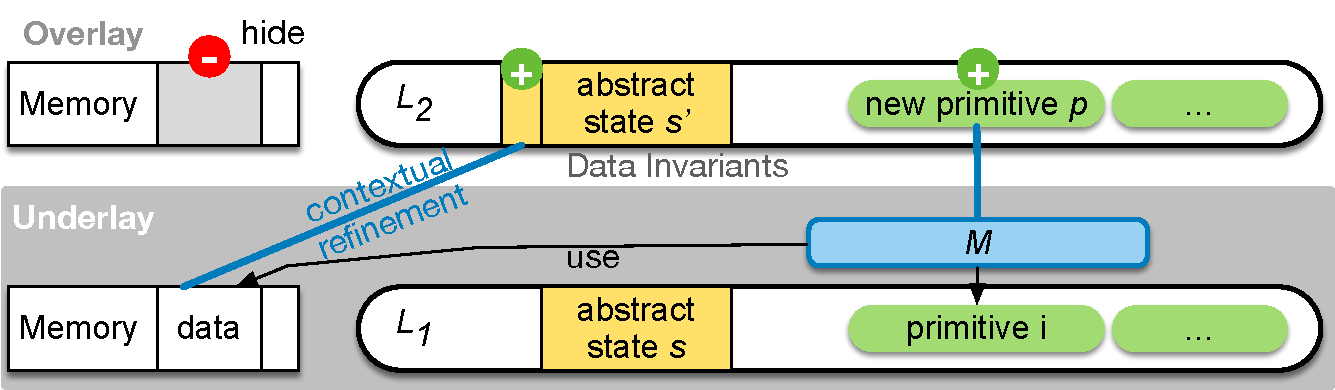
\includegraphics[width=0.8\textwidth]{figs/object-original}
\end{center}
\caption{Layer-based contextual refinement}
\label{fig:spec:object-original}
\end{figure}


Given that $\llbracket{}M\rrbracket{}L_1$ contextually refines $L_2$,
and the deep specifications in $L_2$ captures everything contextually observable
about running $M$ over its underlay $L_1$, we can prove any property of $M$ directly using
the interface $L_2$ alone, and we would never need to look into the actual
implementations in $M$. Since all of our specifications are deterministic
(under fixed external events), the contextual refinement property guarantees
that $\llbracket{}M\rrbracket{}L_1$ and $L_2$ are actually observably equivalent.

Fig.~\ref{fig:spec:object-original} shows the overall idea of the contextual
refinement. As shown in the figure, the code module $M$ may access some
private data in the memory, which corresponds to the new abstract states
in the overlay interface $L_2$. Note that $M$ may also call some of the
primitives defined in the underlay interface $L_1$. The entire behavior
of $M$ is specified as the new abstract primitives in $L_2$ manipulating
the new abstract states in $L_2$ instead. Given that the memory in $L_1$
is replaced by the abstract states in $L_2$, we would like to 
guarantee that the context
code running on the overlay interface does not accidentally damage the private
in-memory data by directly accessing the relevant memory. As shown in
Fig.~\ref{fig:spec:object-original}, we achieve this by utilizing the CompCert
memory permissions~\cite{leroy08} to hide the relevant memory region at overlay,
which prevents the context code from accessing the relevant memory. These
logical permissions do not correspond to any physical protection mechanism, but
are used to ensure that the abstract machine at overlay gets stuck if any code
tries to directly access this portion of memory. The safety proof of our entire
system (the system never gets stuck) guarantees that such a situation never
happens. Thus, the only way to affects the abstracted memory by any context code
running over the overlay interface $L_2$ is to explicitly call relevant
primitives in $L_2$.

\subsection{Downward Simulation}

The contextual refinement is proven by showing a forward
simulation~\cite{Lynch95} between $L_2$
to $\llbracket{}M\rrbracket{}L_1$ over a refinement relation.
In the rest of the chapter, following CompCert, we often call the
forward simulation $\llbracket{}M\rrbracket{}L_1$ (implementation)
to $L_2$ (specification) as {\em upward (forward) simulation} and
the one from $L_2$ (specification) to $\llbracket{}M\rrbracket{}L_1$
(implementation) as {\em downward (forward) simulation}.
The contextual refinement, by definition, requires us to prove
the {\em upward simulation} from $\llbracket{}M\rrbracket{}L_1$
to $L_2$. In practice, the {\em downward simulation} is easier to
achieve, and this is what we prove in our framework. Relying
on the fact that the specifications are deterministic, the proof
is then later turned into the converse {\em upward simulation}
similar to the the way in CompCert.

\begin{definition}[Downward Simulation]
We say that there is a downward simulation from $L_2$ to
$\llbracket{}M\rrbracket{}L_1$ if, and only if, for any
context program $P$ disjoint from $M$, there exists a refinement relation
$R$ over the two states in $\llbracket{}P\rrbracket{}L_2$ and
$\llbracket{}{P \oplus M}\rrbracket{}L_1$ such that, for
every state $(s_2, s_1)$ in $R$, and for every step $st$ in $\llbracket{}P\rrbracket{}L_2$,
if $st$ takes the state from $s_2$ to $s_2'$, then there exists
zero or more steps in $\llbracket{}{P \oplus M}\rrbracket{}L_1$ from
$s_1$ to $s_1'$ such that $(s_2', s_1')$ is also in $R$.
\end{definition}

\subsection{Finding Refinement Relation}

To show the downward simulation, we need to find a simulation relation $R$
such that every step in $\llbracket{}P\rrbracket{}L_2$ can be simulated by
some steps in $\llbracket{}{P \oplus M}\rrbracket{}L_1$.
As shown in Fig.~\ref{fig:spec:object-original}, the relation $R$ can
map the memory and abstract states in $L_2$ to the same memory and abstract
states in $L_1$, with the exception of the part of memory that is hidden in
$L_2$ and the new abstract states introduced in $L_2$. Since the part of
memory is hidden in $L_2$, this part of memory is not mapped to
the same memory containing private data in $L_1$, and in fact it is not
mapped to any state in $L_1$. Instead, the new abstract states in $L_2$
is mapped to the concrete private data in $L_1$'s memory. The concrete
mappings vary depending on the concrete data structures used to implement
the in-memory private data in $L_1$, and the format used to represent
its corresponding abstract states in $L_2$. In the example of the console
buffer, $R$ needs to match the concrete circular array in the memory
to the abstract logical list defined in the layer interface.


\subsection{Proving Downward Simulation}

Based on the definition of the downward simulation, the simulation needs
to be shown for every step in $\llbracket{}P\rrbracket{}L_2$.
Note that the only step that needs special
attention is when $P$ calls one of new primitives introduced in $L_2$.
Because for any other
steps, $\llbracket{}{P \oplus M}\rrbracket{}L_1$ can make exactly same step
to reach a matching state at the underlay.
When $P$ calls any one of the new primitives in $L_2$, this can be simulated
by running the corresponding function defined in $M$ at the underlay.

Thus, in our framework, one only needs to provide the simulation proof
from each overlay primitive $p$ to the corresponding underlay function
implementation $f$, primitive by primitive, with respect to a provided
refinement relation $R$. For each primitive that takes an overlay state
$s_2$ and produces a new state $s_2'$, this proof contains two components.
The first part is to show that from the underlay state $s_1$ that matches to
$s_2$ in $R$, the function $f$ (written either in ClightX or LAsm)
terminates safely and transforms the state $s_1$ to another state $s_1'$.
This step requires us to reason about the function $f$ based on its formal
semantics, and prove that the function does terminate safely (i.e., it
does not get stuck or get into an infinite loop) and produce the return state
$s_1'$. The second part is to show that $s_1'$ is also related to $s_2'$ by $R$.

Instead of mixing these two proof together, our framework provides a way to
systematically isolate these two otherwise related proofs. First, we write
a new specification for each function $f$ in terms of the underlay states.
This specification is called {\em low level specification} in our framework,
in contrast to the {\em high level specification} of the primitive at overlay
in terms of the overlay states. Next, we prove that $f$ satisfies its
{\em low level specification}. This step is called {\em code verification}.
Last, we prove the simulation from the (high level) specification of $p$ to the
{\em low level specification} for $f$ over the refinement relation $R$.
This is called the {\em refinement proof}. The advantage of splitting these
two works are that we do not need to worry about the simulation when we
perform the {\em code verification}, while no code is involved when
we establish the {\em refinement proof}.

A low level specification has a similar type as the primitive
(high level) specification in a layer interface.
As an example, the low level specification for the console buffer
implementation (shown in Fig.~\ref{fig:source:cons-buf}) is shown
in Fig.~\ref{fig:cons_buf_low_spec}.
Here, $\textsf{lspec}~ ge~ args~ (m,~d)~ rval~ (m',~d')$
indicates that under the global environment ($ge$) mapping global variable
identifiers to their locations in the (CompCert) memory, given the argument list
$args$, the function changes the memory from $m$ to $m'$ and the abstract
state from $d$ to $d'$, with the return value
$rval$ ($\textsf{Vundef}$ if no return value). $\textsf{Mem.store}$ is an
operation in the CompCert memory model;  it takes the memory writing type, initial
memory to write to, the memory block, block offset, and a value, and returns the
new memory after writing the value on the location represented by the memory
block and offset on the initial memory. $\textsf{Mem.load}$ is the opposite
operation that loads a value in the specified location of the memory.

\ignore{
As shown in the figure, the low level specifications has equivalent
number of cases as in the source code, and in fact, they are very close
to the source code. Thus, it is relatively easy to show that the source code
satisfies the low level specification shown in
Fig.~\ref{fig:cons_buf_low_spec} and the proof can be achieved nearly
automatically by our proof tactics.
}

\begin{figure}
\lstinputlisting [language = Coq] {src/cons_buf_low_spec.v}
\caption{Low level specifications of the circular console buffer}
\label{fig:cons_buf_low_spec}
\end{figure}


\subsection{Layer Patterns}
As shown in the previous subsection, there are two main components in proving the
downward simulation: the {\it refinement proof} that deals with the relationship
between the overlay abstract states and underlay states, and the {\it code verification}
that handles the verification of actual functional properties of the program.
To further ease the task of developing the layer interfaces and proving the
downward simulation, we have designed and developed two common patterns which
can be used to decompose the problems into pieces so that we only need to focus
on one type of proof at a single moment.

When we introduce and verify a code module, we always first perform {\it data abstraction},
i.e., we abstract the concrete data stored in the underlay memory into a logical
abstract states in the overlay, and provide very simple getter/setter interface in
the overlay to manipulate the new abstract states. The getter and setter methods
are implemented at underlay with simple memory accesses that does not involve much
complex logic or cases. Thus, the {\it code verification} is relatively simple in this case
given the simplicity of the code and similarity between the specification and the
implementation of getters and setters. The main proof focus of this pattern would
be the {\it refinement proof} where we have to show the equivalence of the abstract
and concrete representations of the data. The complexity of this task highly depends
on the complexity of in-memory data structures used and the actual representation
of the abstract states at overlay. It may get very complex when the gap between 
the two representations are relatively large (as in the case of circular console buffer).

Once all the in-memory data are abstracted into logical states at overlay with
the getter/setter interfaces, we implement the actual functional logic on top
of the previous overlay by utilizing the getter/setter primitives whenever
we need to access the new abstract states. Here, the {\it refinement proof}
is trivial as there is no data abstraction, thus the refinement relation is
the {\it identity relation}. The major proof task in this pattern is to perform
the actual {\it code verification}, and we detail our techniques in Chapter
\ref{chapter:automation}.

We have discovered that following the above two patterns significantly reduces the
amount of proof efforts required to prove complex systems by only focusing on one
of the two main proof tasks while completely automating the other.
It also allows us to implement much stronger automation support for each isolated
proof component because, for example, there is no complex code logic involved in the
data abstraction, and the code only manipulates logical states during the
code verification, thus no direct manipulation of the CompCert memory.


\section{Back to Console Circular Buffer}
\label{chapter:framework:console-buffer}

\begin{figure}
	\begin{center}
		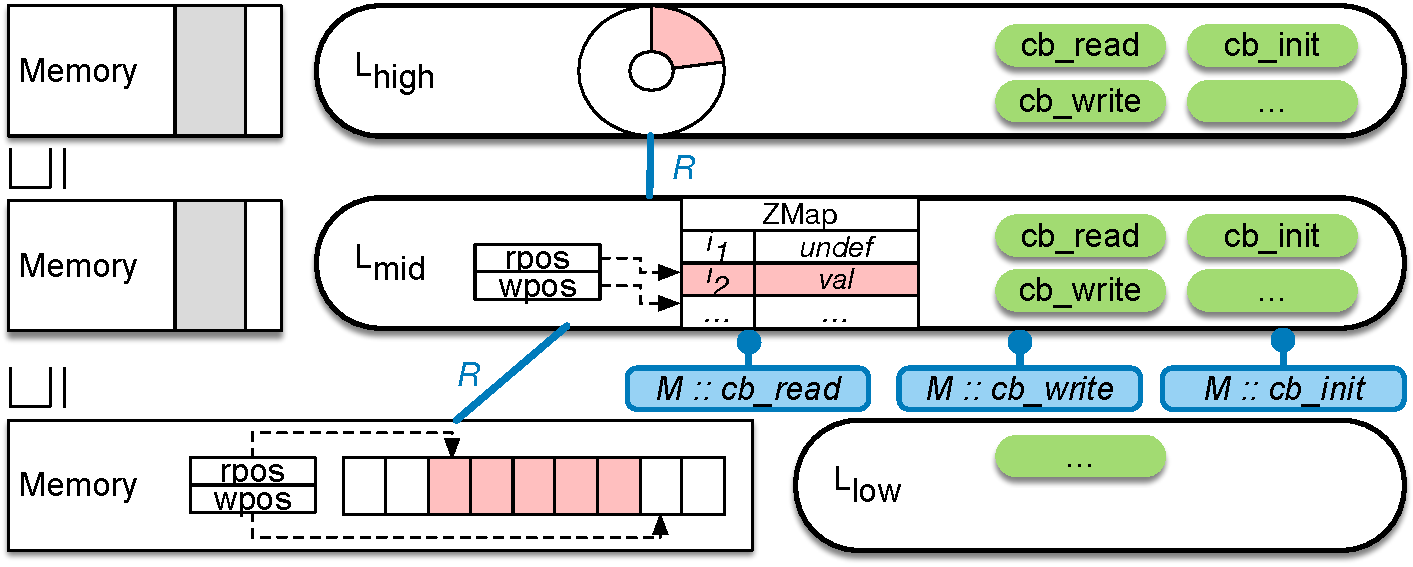
\includegraphics[scale=0.6]{figs/cons_buf}
	\end{center}
	\caption{The layer hierarchy of circular console buffer}
	\label{fig:layer:cons-buf}
\end{figure}

With the support for {\it certified abstraction layers}, we can implement and
specify the circular console buffer, and formally prove the desired property
that the code always satisfies the deep specification in the layer interface.

More formally, let the layer interface defined
in Fig.~\ref{fig:cons_buf_spec} be named $L_{high}$, and the implementation
module in Fig.~\ref{fig:source:cons-buf} be named $M$.
Furthermore, let 
$L_{low}$ define a layer interface when the type of abstract state
is an empty record, and the set of primitives is empty;
$\llbracket{}M\rrbracket{}L$ indicate the behavior of the code module $M$
under the formal semantics of the language $M$ is implemented in (ClightX or LAsm),
instantiated with the layer interface $L$; and $M_1 \oplus M_2$ denote the physical
concatenation of the two individual code modules. Then, the correctness of
the console buffer implementation can be formalized as below:

\begin{lemma}[Correctness of Circular Console Buffer Implementation]
$ $

For every program $P$, there exists a downward simulation from
$\llbracket{}P\rrbracket{}L_{high}$
to $\llbracket{}{P \oplus M}\rrbracket{}L_{low}$.
\end{lemma}

Next, we can define a refinement relation $R$ to relate the concrete circular
buffer in the memory and the abstract list, then prove the contextual refinement
between $\llbracket{}M\rrbracket{}L_{low}$ and $L_{high}$ over the simulation
relation $R$. The forward simulation proof can be achieved on the
primitive-by-primitive basis. One can imagine that due to the non-trivial $R$,
this simulation proof could be complex.

The complexity may further explode when this logical complexity gets mixed with
the complexity of handling the accesses to the CompCert memory. CompCert memory
model is an axiomatized model where the properties are defined through a big
list of axioms without a specific implementation. Any concrete implementation of
this memory model needs to satisfy all the axioms. Thus, one cannot perform any
simple evaluations on the memory, but needs to keep applying appropriate axioms
to derive any desired properties. This severely limits the room for proof
automation and significantly increases the proof size and memory consumption for
proof compilation as the proof gets more complex. To separate the complexity
that comes from the CompCert memory model from the actual complexity of the
proof, in our layered approach, we always make the gap between the underlay and
overlay interface as small as possible when it comes to data abstraction, i.e.,
when a piece of memory gets abstracted into an abstract state at the overlay
interface.

In the case of the circular console buffer, instead of directly jumping from
the in-memory implementation to a logical list, we introduce an intermediate
layer interface where the representation of the circular buffer in the abstract
state is very similar to the one in the memory. We define the intermediate
layer interface $L_{mid}$ with the abstract state $d$ and the primitive specifications
as shown in Fig.~\ref{fig:spec:cons-buf}. Here, for any type $T$, $\mathsf{ZMap}.t~T$
is the type of partial map from integer keys to the values of type $T$.
One can easily observe that the representations shown in Fig.~\ref{fig:spec:cons-buf} are
extremely similar to the actual implementations shown in Fig.~\ref{fig:source:cons-buf}.
Given the similarity, one can easily come up with a refinement relation $R$ which
maps the concrete values in the memory to their appropriate logical values in $d$.
The simulation proof over $R$ is also relatively easy and there is no other
complex factors interfering with the ones from handling the CompCert memory.

Once the contextual refinement between $\llbracket{}M\rrbracket{}L_{low}$ and
$L_{mid}$ is proven, the contextual refinement between $L_{mid}$ and $L_{high}$
can be proven with no code module involved. Thus, this part of proof is completely
logical and the refinement relation $R_{cons\_buf}$ (shown in Fig.~\ref{fig:ref:cons-buf})
in this case only needs to relate two sets of abstract states.
In Fig.~\ref{fig:ref:cons-buf}, \textsf{Abs} is the type of the abstract states
in each layer interface.
The overall layer hierarchy of entire console buffer is shown in Fig.~\ref{fig:layer:cons-buf}.
This kind of two-stage proof strategy
significantly reduces the complexity
of the proof and lifts the main complex proof effort to pure logical level.

\begin{figure}
\[
\begin{array}{lll}
d = ( & \mathsf{cons\_buf\_concrete}: \mathsf{ZMap}.t~\mathbb{Z}, & \vartriangleright \textit{Concrete console buffer} \\
& \mathsf{rpos}: \mathbb{Z}, & \vartriangleright \textit{The head of the buffer} \\
& \mathsf{wpos}: \mathbb{Z}). & \vartriangleright \textit{The tail of the buffer}
\end{array}
\]

\[
\begin{array}{cr}
\inferrule{
	d' = d[\textsf{rpos} \leftarrow 0][\textsf{wpos} \leftarrow 0] \\
}{
	\mathsf{cb\_init} (d) \defeq d'
} & \text{(cb\_init)} \\ [5ex]

\inferrule{
	i = d.\mathsf{rpos} \\
	i \neq d.\mathsf{wpos} \\\\
	c = d.\mathsf{cons\_buf\_concrete}[i] \\
	d' = d[\textsf{rpos} \leftarrow (i + 1)~\textsf{mod}~CB\_SIZE] \\
}{
	\mathsf{cb\_read} (d) \defeq (d', c)
} & \text{(cb\_read\_char)} \\ [3ex]

\inferrule{
	d.\mathsf{wpos} = d.\mathsf{rpos}
}{
	\mathsf{cb\_read} (d) \defeq (d, CB\_EMPTY)
} & \text{(cb\_read\_empty)} \\ [5ex]

\inferrule{
	i = d.\mathsf{wpos} \\
	i' = (i + 1)~\textsf{mod}~CB\_SIZE \\
	d.\mathsf{rpos} \neq i' \\\\
	d' = d[\mathsf{cons\_buf\_concrete}[i \mapsto c]] \\
	d'' = d'[\textsf{wpos} \leftarrow i'] \\
}{
	\mathsf{cb\_write} (d, c) \defeq d'
} & \text{(cb\_write\_char)} \\ [3ex]

\inferrule{
	i = d.\mathsf{wpos} \\
	i' = (i + 1)~\textsf{mod}~CB\_SIZE \\
	d.\mathsf{rpos} = i' \\\\
	i'' = (i' + 1)~\textsf{mod}~CB\_SIZE \\
	d' = d[\mathsf{cons\_buf\_concrete}[i \mapsto c]] \\\\
	d'' = d'[\textsf{wpos} \leftarrow i'][\textsf{rpos} \leftarrow i''] \\
}{
	\mathsf{cb\_write} (d, c) \defeq d''
} & \text{(cb\_write\_overflow)} \\
\end{array}
\]
\caption{Intermediate specifications of console buffer primitives}
\label{fig:spec:cons-buf}
\end{figure}

\begin{figure}
\lstinputlisting [language = Coq] {src/console.v}
\caption{The definition of refinement relation between $L_{high}$ and $L_{mid}$ in Coq}
\label{fig:ref:cons-buf}
\end{figure}



\chapter{Verification of ClightX and LAsm Programs}
\label{chapter:automation}
Given that majority of the system software is developed in C (ClightX
in our case), we need a good framework-level automation support to
verify that ClightX modules meet their (low-level) specifications. 

In the literature, scalable verification support for C programs falls into the following two
categories. One is to transform the proof targets into some lower
level forms and seek help from automation engines like SMT solvers
\cite{boogie05,dafny10}.
The benefits of this approach are that we can discharge the proof goals
nearly automatically without human intervention and this process can be done
very efficiently. On the other hand, this process cannot produce the proof
objects that can be machine checked, thus we would need to trust the implementation
of many of the components in the proof engine, e.g., the underlying SMT solvers.
It is also hard for a human to provide some smart hints in the middle when the
fully automated approach fails or times out.

Another method is to implement some program logic
(Hoare logic, separation logic, {\it etc}) on top of the semantic model where the
set of syntactic logic rules are proved to be sound with respect to the underlying
program semantics \cite{appel11:vst}. There, a piece of C code
is associated with a precondition $P$ that is expected to hold at the entry of
the code segment, and a postcondition $Q$ that should be proved to hold when
the flow exits the code segment. Majority of existing verified systems only prove
partial correctness, i.e., they prove that if $P$ holds at the entry, then either
the program gets into an infinite loop or the program terminates and the exit states
satisfy the postcondition $Q$. Thus, the proof here is termination insensitive.

Our goal is to develop a framework level support on semi-automatically
producing machine-checkable proofs for the correctness of ClightX source programs
against their low-level specifications.
We would like to take the termination seriously as it is critical on artifacts
we are interested in, e.g., an operating system kernel.
More importantly, we try to make
the linking of different semantic components and modules to be uniform, and more importantly,
explicit, to remove any potential semantic gaps among different modules.
We use simulation as the uniform formalism. For example, we prove that
the C program is a simulation of the low-level specification (C code verification), 
the assembly program is a simulation of C (compiler correctness), {\it etc}.
The transitivity of simulation allows us to naturally compose all the
proofs together formally, and explicitly in Coq.
With the Hoare logic approach, it is unclear how we can formally link the compiler
correctness theorem with the Hoare triple to derive a combined theorem about
the compiled assembly program, and it is also unclear how you can further link
that correctness theorem with another program written and proved directly
at the assembly level.

Fig.~\ref{fig:cons_buf_code_lemma} shows our main lemma for the correctness of
the circular console buffer accessor functions against their low-level specifications
shown in Fig.~\ref{fig:cons_buf_low_spec}. As shown in Fig.~\ref{fig:cons_buf_code_lemma},
we prove the {\it downward simulation} from the specification to implementation, i.e.,
we prove that the code is a simulation of its low-level specification.
While this is very different from traditional Hoare logic approach, it links
nicely with the downward simulation we prove for the {\it refinement proof}
and we turn the entire downward simulation in the end into a final upward simulation
for the contextual refinement. 

With the certified abstraction layers, we manage to systematically guarantee
memory isolation through abstract states and primitives, and the invariant preservation
by enforcing invariants on the abstract states that are preserved by the primitives.
In addition, we can perform the complex functional correctness logic at the
pure logical level with the abstract states and primitives.
In this chapter, we show how we develop a collection of strong automation tactic
libraries that can efficiently prove the downward simulation from the low-level
specifications to their implementations.

\begin{figure}
\lstinputlisting [language = Coq] {src/cons_buf_code_lemma.v}
\caption{Lemmas for the correctness of console buffer implementation}
\label{fig:cons_buf_code_lemma}
\end{figure}

\section{Design Principle}
\label{sec:principle}

In our framework,
code verification is achieved semi-automatically through Coq tactic libraries
implemented in the Coq's tactical language \emph{Ltac}. 
The automation engine is designed and implemented with special emphasis on
the scalability and usability, with the intention to use it in large-scale
low-level system verification like operating system kernel.
While as any other automation support, the main goal is to reduce manual proof as much as
possible and seek for human interaction only when it is necessary,
the system is designed with the following desired properties in mind.

\paragraph{Easy to pick up}

It is never practical to achieve verification of large-scale system software
with one-man effort. One of the main goals is to make it simple and intuitive
to use and maintain the developed tactic libraries. 
The automation library implementation consists of many small library modules, which
makes it more easy and intuitive to debug and extend the library by someone
other than the initial developer. On the other hand, I have developed a top-level
all-purpose tactic called {\it cauto} which repeatedly performs the top-level
pattern matches and calls into appropriate lower level libraries.
Thus, in many cases, users can simply invoke this tactic without worrying about
what specific tactics should be used for the particular subgoal that pops up.

The tactics can fail, mostly due to careless mistakes in specification or implementation,
e.g., type mismatch, wrong variables due to typos, {\it etc}. In order to figure
out the causes and fix them, one may need to debug the tactics. Coq is known to
have poor support for debugging Ltac. The default Ltac debugging mode does not
work well in practice. Without any additional debugging support, the known best
practice is to copy and paste the tactic source code into the proof script
and debug part by part to figure out which part caused the failure.
We still have to do that in our proof in some cases, but we also identified
some common mistakes and failing tactics and developed a ``test'' version of
the tactics that fail gracefully when
something goes wrong. Thus, in many cases, when we see that the main tactic
fails, we invoke the test version which does not fail and leave some intermediate
state that prevented the main tactic to proceed, which can be used to determine
the source of errors much easier.


\paragraph{Sound}
Coq is sound, given its underlying core is sound, which is reviewed and exercised
by many experts and members in and outside the community. On the other hand,
that does not prevent our Ltac proof scripts to enter a situation that the remaining
subgoals are not valid. One major source of such a situation could happen when we
deal with {\it existential variables}. 

Existential variables are placeholders for
variables that are not instantiated to concrete values yet and are
denoted by a numbered question mark, e.g., $?77$. Variables with different numbers
denote different existential variables, but they can later be instantiated to
the same value. They can be introduced explicitly by the proof script with
tactics like \textsf{esplit}. For example, when we have a proof goal of
$\exists~x,~x=7$, we can first run \textsf{esplit}, which replaces the existentially
quantified variable $x$ with an existential variable (e.g., $?8$) and turns the
goal into $?8=7$. The existential variables can also be (and are mostly) introduced
automatically for each of intermediate variable that Coq cannot immediately
deduce its value while running tactics like \textsf{eapply}.
For example, if we have a theorem \textsf{trans\_f} of the form
$\forall~x~y~z,~f(x,y)~\rightarrow~f(y,z)$ and our current subgoal is $f(1,2)$,
if we run ``\textsf{eapply} \textsf{trans\_f}'', Coq would not be able to
automatically deduce the value of $x$, and it would turn the goal into
$f(?5, 1)$.\footnote{The number in the existential variable is assigned by
Coq and does not have any intended meaning.}

Existential variables can be instantiated explicitly by the \textsf{instantiate}
tactic. In the case of $?8=7$ above, we can first run
``$\textsf{instantiate}~(1:=7)$'' to instantiate the right-most appearance of
existential variable (in our case, the only variable $?8$) to $7$ and turn
the goal into $7=7$, which can be solved easily by the \textsf{reflexivity} tactic.
On the other hand, Coq itself also tries to fill the existential variable
whenever it finds a suitable candidate. In the above example, we can directly
run \textsf{reflexivity} on $?8=7$ which can automatically instantiate
$?8$ to $7$ and solves the goal.

The existential variables give us a convenient way to not to spell out many
temporary states that we do not care about and let the automation engine
automatically deduce the values during the proof. Without them, we would need
to explicitly come up with all these intermediate values and provide it when
we apply various theorems or lemmas. In addition to the intermediate temporaries
get generated during the proof, we can also omit some states that is not
relevant to what we prove. For example, in Fig.~\ref{fig:cons_buf_code_lemma},
the final temporary environment after the code execution ($le'$) is existentially
quantified, as it is about to be thrown away and not relevant to our specification
that is stated in terms of memory and abstract states.

On the other hand, existential variables can become the main evil that hinders
more aggressive optimization. In general, when our automation tactic stops,
we either want the goal to be solved completely, or the leftover subgoals
should be provable semi-automatically with some human interactions.
If the tactic call results in inconsistent states that are not provable,
then the only choice we have is to debug the tactics to prevent that from
happening. This is particularly not suitable in large-scale system verification,
where the same automation libraries are used by many different components
(or even different systems) developed by different members of the team.
Instead, we strictly enforce that the remaining goals should always be valid
when the tactic call terminates. This means that we do not aim to achieve
an aggressive push-button or single-attempt verification where a single tactic
call tries to solve the entire goal. Instead, our tactic stops whenever
there is any potential for making wrong decisions. One typical example would
be running simple tactics like \textsf{reflexivity} on a goal with expressions
containing existential variables. For example, when we have two subgoals
$?11\le5$ and $?11=4$, if we apply \textsf{reflexivity} to $?11\le5$ first,
Coq would instantiate $?11$ with $5$ and discharges the first goal, and
we end up with a goal $5=4$ which is not arithmetically valid. Instead,
our tactic would stop on the first goal since there are more than one choices
of $?11$ that is less than $5$. On the other hand, it does not stop on the second
goal because there is only one possible instantiation that makes it equal to $4$.
Thus, it would still make process on the second goal, which allows our repeating
engine to continue and automatically solve the leftover goal ($4\le5$).
Unfortunately, this is not always the case. In this chapter, I present
more examples in detail and discuss potential drawbacks and ways to overcome
them.


\paragraph{Reasonably efficient}

We cannot expect the performance of our Ltac scripts to be comparable
to the SMT solvers. But we would still expect them to be
reasonably efficient so that it does not hinder its usability in practice.
If every tactic call to \textsf{cauto} takes minutes to respond on average,
it would not be practical to use it in large-scale verification.
It is possible that we write an extremely lengthy function with the
corresponding proof script to take hours to compile. But here we are
concerned about a function at a reasonably small size since the majority
of functions in an even complex system software should be reasonably small,
otherwise, it was not implemented following a modular design.
Among those small size functions, some of them are very short (less than
ten lines of code), where we should expect our automation tactic to
finish within a couple of seconds. For the ones with longer size,
we probably would expect it to take no longer than a couple of minutes.

Even though we do not enforce any time requirement for our tactics,
we have made some design decisions to make the tactics reasonably more
efficient.

First, we try to organize the tactics info many different modules.
Recall that the pattern match in Ltac scans and tries each case
linearly, moves to the next branch when the tactic execution
at the current branch fails, and stops at the first case that
the corresponding tactics do not fail. Thus, by organizing the
tactics into the components, we manage to turn the overall structure
into search trees instead of a linear list.

Second, application of tactics may results in new subgoals unless
it solves the goal completely. We would like to discharge these
subgoals on the fly as soon as they become provable by themselves.
This limits the number of subgoals exists in any moment of proof, thus
prevent the size to explode and also reduces memory consumption
significantly. Discharging subgoals sooner also accelerates instantiations
of existential variables, thus preventing the tactics to spin out
more and more existential variables based on existing ones, which
reduces the likelihood of the tactic stopping due to the existential
variables. Thus, we integrate the main tactic with many kinds of theory solvers
(again implemented in Ltac) to discharge subgoals as soon as we can.

Third, we try not to be too smart. Even in some cases, where it would generally
make sense to proceed the proof in certain ways unless it is guaranteed to
be always the right choice, we would rather let
the tactic to stop and let the user make the right decision. This principle
holds even when proceeding the tactics does not result in inconsistent states.
We would prefer to let the user make the right decision by invoking the right
tactics later rather than letting the tactic potentially waste time trying
various approaches then eventually times out.

Last but not the least, we try to only support the cases that are most commonly
used in our main top-level tactics. We would like to support the full
features of ClightX in our library so that it can be used to verify arbitrary
system software written in ClightX. On the other hand, there are many
C features that are not used often. If we include all these cases in the
main tactic path, then it would slow down the entire pattern matching process
with these extra cases that rarely hit, thus making the entire proof slow to compile.
Note that this would be true even if we put these relatively rare cases
at the end of the pattern match list. The top-level tactics are applied
repeatedly on all the current subgoals to check whether any of the subgoals
can progress with the tactics, and while it progresses at some subgoals, for
many of others, it would go through entire pattern match list before the tactics
fail on these goals. Thus, I only include cases to handle most common ClightX
constructions in the main high-level tactics.
On the other hand, I have also developed separate tactics to handle the rest
of constructions that have relatively rare usage, and also the actual top
level tactics that include all these, which can be convenient if the performance
of the current proof is not the bottleneck.


\section{Overall Approach}
\label{sec:approach}

Our basic idea is simple. Given a proof goal like one shown in Fig.~\ref{fig:cons_buf_code_lemma}, we can repeatedly apply the big-step
semantic rules shown in Fig.~\ref{fig:clight_eval_expr}, \ref{fig:clight_exec_stmt},
\ref{fig:clight_exec_stmt2}, and \ref{fig:clight_outcomes} to decompose all
the Clight expressions and statements into smaller ones together with
the extra conditions required for the evaluation or the execution as subgoals.
This procedure is called the verification condition generation. 

Take a simple example, the implementation of \texttt{cb\_init} (see
Fig.~\ref{fig:source:cons-buf}) is a simple sequential composition of
two assignment operations. To verify the corresponding low-level specification
\texttt{cb\_init\_lspec} shown in \ref{fig:cons_buf_code_lemma}, we can first
remove the existential quantifier by replacing it with an existential
variable (with \textsf{esplit} tactic). Then we can turn the sequentially
composed statement into two individual statements by applying the rule
\texttt{exec\_Sseq\_1} shown in Fig.~\ref{fig:clight_exec_stmt} (with
the \textsf{eapply} tactic). Furthermore, the individual assignment
statements can be turned into appropriate smaller subgoals
by applying the rule \texttt{exec\_Sassign} shown in
Fig.~\ref{fig:clight_exec_stmt}, and we repeatedly follow this approach
by applying applicable rules shown in Fig.~\ref{fig:clight_eval_expr},
\ref{fig:clight_exec_stmt}, \ref{fig:clight_exec_stmt2}, and
\ref{fig:clight_outcomes}, and discharge simpler subgoals as soon as
they become provable by themselves with the current assumptions.

Though it sounds reasonably simple, there are many nuances that require extra
careful thoughts. 
In the rest of the sections, I discuss various components of our tactic libraries
and discuss such challenges and our solutions in more detail.
In addition, the language Clight strictly follows the C standard and disallows the
undefined behaviors described in the standard C semantics. Thus, these all
become the preconditions in the semantic rules of the Clight language. For a
reasonably realistic C module, the set of verification condition generated is
extremely large. Thus, discharging the conditions after they are fully generated
would be very inefficient. In the following sections, I also introduce the list of
theory solvers I have designed to discharge the sub-goals of various forms
on the fly as soon as they become provable.


\section{Simple proof}

When the goals get down to very simple forms, e.g., simple equalities or inequalities,
goals that are already known in the assumptions, {\it etc}, we would expect to
discharge them easily with a tactic like \textsf{reflexivity}, \textsf{assumption/eassumption},
\textsf{omega}, and so on. On the other hand, as we discussed in Section \ref{sec:principle},
randomly applying these tactics could lead us to non-provable subgoals, due to the
existential variables. Fortunately, Coq provides two tactics \textsf{is\_evar v}
and \textsf{has\_evar e} which only succeed if the provided variable is an existential
variable or the expression contains any existential variable, respectively.
Fig.~\ref{fig:simpleproof} shows our approach to instead invoke the ``safe'' versions
of \textsf{reflexivity} and \textsf{eassumption} utilizing these tactics.
For example, \textsf{sreflexivity} only calls \textsf{reflexivity} on true equalities,
but not in the case of inequalities. On the other hand, \textsf{seassumption}
only calls \textsf{eassumption} tactic when it thinks it is safe to do so.
In the figure, \textsf{isn\_evar v t} only calls the tactic t if \textsf{v} is not
an existential variable, and fails otherwise; while \textsf{hasn\_evar e t} would only
call \textsf{t} if the expression \textsf{e} does not contain any existential variables.

\begin{figure}
\lstinputlisting [language = Coq] {src/simpleproof.v}
\caption{Discharging simple proof goals with potential existential variables}
\label{fig:simpleproof}
\end{figure}

With this approach, in many cases, we could cause the automation engine to stop early,
even when it has the ability to instantiate many existential variables correctly.
Then after invoking the main tactic \textsf{cauto}, the human prover needs to
instantiate the existential variables that caused the stop (or instantiate
any many remaining existential variables as she can), and reinvoke \textsf{cauto}
tactic. However note that the first \textsf{cauto} may result in a huge number
of unproven subgoals, and once we are done with the instantiation, we need to call
the equivalent number of \textsf{cauto} tactic to prove the rest of subgoals.
This list may grow exponentially and result in an unnecessarily lengthy proof
script of \textsf{cauto} call chains.
Instead, in practice, I normally chain the calls to the proof tactics, e.g.,
$\textsf{cauto};~[\textsf{idtac}~|~\textsf{do\_right\_thing}~|~\textsf{idtac}];
~\textsf{cauto}$. 
Recall that a call to $t_1;t_2$ would apply the tactic $t_2$ to all the remaining
subgoals after the $t_1$ tactic call; $[t_1;t_2;...t_n]$ notation allows
us to specify which tactic we would like to invoke on each remaining individual
subgoals; and \textsf{idtac} is a tactic that does nothing and always succeeds.


\section{Sequential code}

Sequentially composed code sounds easy to deal with, as we can simply
decompose it into its subcomponents. On the other hand,
if we look at the semantic rules in Fig.~\ref{fig:clight_exec_stmt}, there are
two separate rules for the sequentially composed code. In addition to the rule
\texttt{exec\_Sseq\_1} that covers the normal execution of two statements
one followed by the other, we also have the rule \texttt{exec\_Sseq\_2},
where the first statement terminates by \texttt{return} or \texttt{break}
(when the statement is within a loop) statement, and the whole statement
terminates without executing the second component.

In order to automate the proof, we need an effective way to decide which
of the two rules we should apply when we hit the sequentially composed statements.
This could be extremely hard to achieve, as we may have statements of form
$\{s_1;~s_2;\}~\{s_3;~s_4;\}$, where $s_1$ or $s_2$ may contain branches,
which makes it not feasible to determine whether the first component would exit
normally or not without evaluating the actual branching expressions.
On the other hand, recall that our ClightX source code is automatically generated
by the tool \texttt{clightgen} from the standard C source code, and \texttt{clightgen}
always turns the sequentially composed statements into the form
$s_1;~s_2;~s_3;~s_4;$, which prevents many troubles automatically determining
appropriate rules. Still, if we hit the statement of the form $if(e)~return;~s;$,
it would be hard to determine the cases without actually evaluating the expression
$e$. Instead of getting into the battle of various efforts/heuristics to determine
the set of tactics that work for all these cases, our main automation tactics
always chooses the normal case whenever it gets confused. This would mean that
we need to stick to a certain C coding standard in order to gain full automation.
On the other hand, we do not obverse much inconvenience by sticking to only
non-ambiguous forms.

\section{Branches}

Handling branching code needs special attention. Naively applying the logical
rules in Fig.~\ref{fig:clight_exec_stmt} repeatedly would not work, because,
the same branching condition can only be evaluated to either true or false,
but not both, i.e., all the existential variables for the uncertain values
cannot be instantiated more than once with different values.
This would mean that all branching decisions should be fixed before we introduce
any existential variables. 

One way to solve the issue is to design a custom programming logic that does
the branching for us and gives us two separate goals to solve for the two branches.
The challenge here is that in order to separate these two goals nicely, it would
force us to explicitly provide many temporary or final states that we do not care
about, e.g., the intermediate states during the execution of statements (which
was automatically derived with existential variables), and the final temporary
local environment $le'$ in Fig.~\ref{fig:cons_buf_code_lemma}.

Instead, in our framework, we simply require all the case split to be done upfront,
to generate separate full subgoals for various branches, before we start our main
proof. We found that, in practice, this does not bring us much inconvenience as
it sounds in the first place. The primary reason is that we always insist to
write deep specifications to capture everything we would like to know in the
implementation, and thus in most cases, the specification also contains branches
when the implementation does. In this case, we simply perform the inversion
on the specification to get separate subgoal for each branch.

One potential inconvenience is that when the implementation contains a big
chunk of common code that is shared among branches, we may end up doing
same proof multiple times if the proof is not done properly. On the other
hand, we simply overcome this by extracting and proving the common part once
as a separate lemma.

\section{Loops}

It is obvious that loops need special treatment, as otherwise, we would keep
applying the semantic rules in Fig.~\ref{fig:clight_exec_stmt} indefinitely.
Instead, I have developed various separate logic modules for loops.
An example module of proving simple while loops is shown in Fig.~\ref{fig:loop_proof}.
As shown in Fig.~\ref{fig:loop_proof}, each of such modules is parameterized
over a precondition $P$ (which is expected to hold at the loop entry), and
a postcondition $Q$ (that needs to be proved to hold at loop exit).

Recall that we enforce total correctness, thus always need to prove that
the loop does terminate. This is achieved by enforcing a termination metric that
``decreases'' at every iteration.
For example, the module in Fig.~\ref{fig:clight_exec_stmt} requires a termination
metric of type $W$ with some sort of ``less than'' relation $lt$, and a proof
that the relation $lt$ is actually well founded.


\begin{figure}
\lstinputlisting [language = Coq] {src/loop_proof.v}
\caption{Framework for proving a simple while loop}
\label{fig:loop_proof}
\end{figure}

Another important input to the module is the loop invariant $I$, which is
a relation over the changing state (memory and temporary environment), and
the termination metric. We are required to provide two proofs.
First, the state at the loop entry satisfies the loop invariant $I$,
if it satisfies the precondition $P$ ($P\_implies\_I$).
Next, if the state before a particular iteration satisfies the loop
invariant, then either the loop condition evaluates to false, causing
the loop to exist with an exit state satisfying the postcondition $Q$,
or the loop condition evaluates to true, and the loop continues, with
states after this loop iteration still satisfy the loop invariant $I$,
with a new termination metric that is ``less than`` the original one.

With all these inputs, we can successfully derive the theorem
{\em termination} in Fig.~\ref{fig:loop_proof} that states
if the state at loop entry satisfies the precondition $P$,
then the loop always terminates safely and the final state
satisfies the postcondition $Q$. The proof can be achieved
by performing induction on the termination metric and doing
case analysis on whether the loop condition would be evaluated
to true or false at this iteration. Intuitively, the termination
is guaranteed because the metric ``decreases'' at every iteration,
but cannot decrease indefinitely because of the well-founded order.

With this framework support for loops, we always perform the verification
of individual loops as separate lemmas that get applied when we prove
the main code that contains the loops. Our main automation tactic
seeks for an applicable lemma whenever it gets to a loop, and stops
if it finds no appropriate lemmas to apply.

\section{Arithmetic Solver}

The standard {\em omega} tactic is too weak to handle many arithmetic
goals appear in our proof. The user code may contain many arithmetic
operations that involve non-linear and bit-wise operations.
To prevent the overflow, the Clight semantics requires every
intermediate value in the middle of expression evaluations to be within the
range regarding its type. In this way, most of the Clight code generates a huge
set of arithmetic sub-goals for checking value ranges. We have incorporated
the {\em cauto} tactic a powerful arithmetic solver that can handle divisions,
modular operations, bit-wise operations, machine finite precision integers, {\it
etc}. 


\section{Partial Maps and Lists}

Clight semantics also utilizes partial maps and Coq lists to represent the local
variable environments and arguments. Furthermore, we extensively use partial
maps and Coq lists in the abstract states to abstract many of the concrete data
structures in memory. To support those, the tactic contains theory solvers to
discharge proof goals for properties related to partial maps and Coq lists. The
tactic also contains a number of domain-specific libraries which handle items
such as device transitions and logs.

\section{Back to the Circular Console Driver}

With our automation tactic libraries, verification of C functions become
reasonably simple.  Given the proof targets like the examples shown
in Figure \ref{fig:cons_buf_code_lemma}, we normally need to first
invert the low-level specifications into concrete premises, apply
the main automation tactic \textsf{cauto}, then discharge the remaining
subgoals with some human intervention, with some special care on the
branches and loops.

\begin{figure}
\lstinputlisting [language = Coq] {src/cb_init_proof.v}
\caption{Verification of the \textsf{cb\_init} implementation}
\label{fig:cb_init_proof}
\end{figure}

As an example, verification of the function \textsf{cb\_init} is shown
in Figure \ref{fig:cb_init_proof}. Here, we first call the tactic \textsf{intros}
to introduce the variables appearing with \textsf{forall} as well as the
premise for the low-level specification; turn the final temporary environment
\textsf{le'} into an existential variable through the \textsf{esplit} tactic;
invert the low-level specification premise into concrete memory
store operations (see Figure \ref{fig:cons_buf_low_spec});
unfold the function body definition; invoke our main automation
tactic \textsf{cauto}; and lastly, discharge the remaining subgoals
by converting the \textsf{Int.repr 0} into equivalent form of \textsf{Int.zero}
that we used in our low-level specification.

Note that the tactic is not trying to be smart and check the equivalence between
\textsf{Int.repr 0} and \textsf{Int.zero}. As our tactic is invoked repeatedly a
large number of times, we would not want to try various attempts and
fail later when we figure out they did not work out. On the other hand, if
we would have some relations repeated in many subgoals, we can assert
them in advance before we invoke \textsf{cauto}, and the tactic is able
to utilize the asserted premise properly in the proof.

The verification of \textsf{cb\_read} and \textsf{cb\_write} are similar except
they contain branches. As we illustrated before, when a function contains
branches, the corresponding deep specification normally also contains the equivalent
number of cases. Thus, we would need to first invert the low-level specification
to obtain multiple subgoals corresponding to different branches of the code,
and discharge the goals separately with the \textsf{cauto} tactic.

The console buffer code does not contain any loop as it only contains simple
getter and setter methods. Examples on verification of C functions with loops and nested
loops are covered in Chapter \ref{chapter:sequential}.

\section{Evaluation}

The automation library is used extensively to prove many
lines of C code in various verified system software,
e.g., the verified sequential OS kernel, the verified
interruptible kernel with device drivers, the verified
concurrent OS kernel with fine-grained locking,
the verified kernel with real-time support, the verified filesystem, {\it etc}.

Within those projects, the library is exercised by many (undergraduate and graduate)
students and (postdoctoral) researchers in our group.
Some of them have few or no
experiences in the Coq proof
assistant, yet they picked up the library and started to perform code verification
reasonably quickly after they obtained some basic knowledge of Coq.

To give some statistics, it took about 30,000 lines of Coq code to verify
the 3,500 lines of C code in the interruptible kernel, and about
52,000 lines of Coq code for the 6,500 lines of C code in the concurrent kernel.
The ratio between the number of lines of proof script and the implementation
may seem a bit high, but it includes all the intermediate specifications and lemmas.
And a relatively large number of proof scripts are dedicated to proving some
outliers with some non-trivial nested loops and logics.
In general, the functions in various kernel components are reasonably simple and
can be automated completely.


\section{Verification of LAsm functions}
We have also developed an automation library to provide some
automation support in proving the modules directly implemented in LAsm.

The very high-level idea in the tactic implementation for LAsm language
is very similar to that in ClightX, i.e., we apply various semantic rules
in its operational semantics (see Fig.~\ref{fig:lasm_semantics}) when we
hit each of its statements.
On the other hand, the assembly code is much
less structured in nature compared to the ClightX programs, and it
does not (and cannot) have a nice big-step semantics as in ClightX.
The automation tactics we have developed for LAsm is not
as mature or as powerful as the ones for ClightX. For example, we only
have many small tactics that we can use to manually apply for various
statements and common patterns, but does not have a top-level ``clever''
tactic that tries to automatically apply various smaller tactics to
solve the entire goal. In practice, we find it to be good enough
since the part of system code directly implemented in assembly
is normally relatively small.

\chapter{Case Study: Verification of the mCertiKOS Kernel}
\label{chapter:sequential}
To illustrate the effectiveness of our automation engine, in this chapter, we present
how we build, specify, and verify each of the mCertiKOS kernel functions using the tools.
We first present the lowest level machine model, the layer interface MBoot.

\section{Machine Model}
\paragraph{Layer Interface MBoot}

\begin{figure}
\lstinputlisting [language = Coq] {src/mboot_rdata.v}
\caption{The abstract states in the layer interface MBoot}
\label{fig:ref:mboot_rdata}
\end{figure}

The interface MBoot is the lowest level layer interface in mCertiKOS, which is
used to model the behaviors of hardware and the unverified boot loader.
The abstract states of the MBoot interface is shown in Fig.~\ref{fig:ref:mboot_rdata}.

On an x86-based systems, the BIOS reports the physical memory information
through the \textsf{e820} memory map to allow the operating system to figure out
which memory address ranges are usable and which are reserved for use by the BIOS.
The \textsf{e820} table consists of a sequence of triples $(s, l, p)$, indicating
the starting address $s$, the length $l$ of the region from the address $s$, and
the permission $p$ (whether the region is reserved by BIOS or not). This triple
is represented by the abstract type \textsf{MMInfo} in Fig.~\ref{fig:ref:mboot_rdata}.
Since this data is initialized by the boot loader, the
\textsf{MMInfo} in Fig.~\ref{fig:ref:mboot_rdata} also contains the default case
\textsf{MMUndef} to indicate the case when it is not yet initialized by the boot loader.
The whole \textsf{e820} table is represented by \textsf{MM} as a partial map
from integer keys to \textsf{MMInfo}. Since it is a partial map, the number of
\textsf{MMInfo} entries is defined separately as \textsf{MMSize} as shown in
Fig.~\ref{fig:ref:mboot_rdata}.

The MBoot interface also defines a list of primitives to operate on the abstract
memory map. The primitives \textsf{get\_mms}, \textsf{get\_mml}, and \textsf{is\_usable}
receives an integer $i$ as parameter and returns appropriate field in \textsf{MM}
with the key $i$, while the primitive \textsf{get\_size} returns the number of
entries in the table.

There are also three abstract states in MBoot related to the hardware paging.
The abstract state \textsf{CR3} models the hardware \textsf{CR3} register,
which stores the root address of the current page table; the abstract state
\textsf{ti} models the hardware \textsf{CR2} register that stores the fault address
when page fault happens; while the abstract state \textsf{pg} represents
the hardware \textsf{CR0} register indicating whether the paging is turned on or off.
Appropriate primitives are also defined in MBoot to set these states.

The special flags \textsf{ikern} and \textsf{ihost} represent whether the execution
is currently in the kernel and host mode, respectively. They are set to \textsf{true}
when the execution traps into the kernel or host, and are set to \textsf{false} when
the execution returns back to user or the guest.


\begin{figure}
	\lstinputlisting [language=Coq] {src/bootloader.v}
	\caption{The specification of \texttt{boot loader} in Coq}
	\label{fig:bootloader_v}
\end{figure}

The special flag \textsf{init} represents whether the kernel data is fully initialized.
Verification of initialization code has always been a big challenge because the system
data would only satisfy global invariants when they are properly initialized by these code.
In other words, the invariants are not satisfied when these initialization code run but
are established through these initialization process. Existing verification approach
has assumed that all the system data are already properly initialized, thus leaving
all the initialization code unverified \cite{klein2009sel4,klein14}.

To tackle this challenge, we build the initialization stack into a hierarchical structure
instead of the standard flat structure, i.e., each initialization function always first calls
the previous initialization function, then initializes its underlying data. At the bottom layer,
we have the specification of the boot loader, which initializes the \textsf{MM} and \textsf{MMSize}.
Like any other initialization functions, it requires the \textsf{init} to be \textsf{false} at entry, and turns
it to \textsf{true} upon exit. Then all invariants relying on initialized states require that the \textsf{init}
being \textsf{true}, i.e., the the data are properly initialized by corresponding initialization function.
For example, we have following invariant on the \textsf{MM}.

\begin{invariant}[MM valid]
If \textsf{init} is \textsf{true}, for any index $i$ such that $0\le i<MMSize$, we have valid memory mapping
triple of $(s, l, p)$ where $s >= 0$, $l > 0$, and $s + l < Int.max\_unsigned$.
\end{invariant}

Since the MM table and its size comes from BIOS, the invariant is treated as top level
assumption of our entire proof on the correctness of the BIOS. 

Each layer interface has exactly one initialization primitive, e.g., either just gets passed through
from the previous layer interface or a new primitive that is newly introduced in this layer
interface, and since this primitive sets \textsf{init}
to \textsf{true} from \textsf{false}, this primitive needs to initialize all the proper abstract states
such that the initialized states satisfy all the invariants in this layer interface.

Figure \ref{fig:bootloader_v} presents our Coq specification for the boot loader primitive.
Here, the notation ``\textsf{adt \{attr: val\}}'' indicates a new abstract state where the attribute
\textsf{attr} in \textsf{adt} is replaced by the new value \textsf{val} and otherwise the same
as original \textsf{adt}.
The specification is written as a function which takes the abstract data type \textsf{RData},
and returns a new abstract state or \textsf{None} representing the execution gets stuck.
Our top level specification guarantees that the system execution never gets stuck.
But at this level, the primitive could get stuck when this primitive is misused, e.g., when it is called twice.


\section{Physical Memory Management}

In physical memory management module, we build a physical page allocation map to maintain the
allocation status of physical pages.
The top section in Figure \ref{fig:at_v} shows
the C implementation of the allocation table, where each allocation entry contains the field \textsf{isnorm}
to indicate whether the
physical page is reserved by BIOS, reserved for kernel usage, or free to be used by user programs;
and the field \textsf{allocated} to indicate whether the page is already allocated by the kernel.

\paragraph{Layer Interface MATIntro}
We would like to initialize the allocation information map with the information from the \textsf{MM},
and provide an allocation method to allow the kernel to allocate a physical page.
Before we implement and verify all these functions, following our mantra, we would like to perform
these reasoning completely at the logical level, without worrying about isolation.
As shown in the bottom section of Figure \ref{fig:at_v}, we introduce a new layer interface MATIntro
to abstract the concrete in memory allocation table into a logical map. Here $ZMap.t$ is a partial
map implementation which takes a value type and returns a partial map from integers to the values of given type.

In this layer interface, we provide several getter/setter primitives to operate on this map:
\texttt{at\_get} and \texttt{at\_set} primitives to read and write to the \textsf{allocated} field of \textsf{AT},
and \texttt{is\_norm} and \texttt{set\_norm} for the \textsf{isnorm} field. \texttt{set\_norm} also sets \textsf{allocated}
to \textsf{false} in addition.


\begin{figure}
	\lstinputlisting [language=Coq] {src/at.v}
	\caption{The in-memory and logical representation of allocation table}
	\label{fig:at_v}
\end{figure}

\paragraph{Layer Interface MATInit}

\begin{figure}
	\lstinputlisting [language=C] {src/mem_init.c}
	\caption{The implementation of \texttt{mem\_init} in C}
	\label{fig:mem_init_c}
\end{figure}


\begin{figure}
	\lstinputlisting [language=Coq] {src/mem_init.v}
	\caption{The specification of \texttt{mem\_init} in Coq}
	\label{fig:mem_init_v}
\end{figure}

Next, we would like to initialize this logical allocation table using the information provided
in \textsf{MM}. The concrete C implementation is shown in Figure \ref{fig:mem_init_c}.
Note that as we discussed earlier, first thing it does is to call the lower level initialization
function (boot\_loader in this case) before it performs the actual initialization of its data.
As shown in the figure, it contains two main components. It first computes how much memory
do we have on this machine and sets \textsf{nps} field properly by calling the \texttt{set\_nps} primitive.
Next, it sets proper allocation state for every page based on the information available in \textsf{MM}.
The corresponding Coq specification is shown in Figure \ref{fig:mem_init_v}. 
Comparing to the specification of \texttt{boot\_loader}, the difference is that it also initializes
\textsf{AT} and \textsf{nps} fields in the abstract states to their expected logical values.

The verification of this initialization function is not trivial. But fortunately, our reasoning
is now completely at logical level and there are no in-memory data involved, thus no need
to reason about isolation as they are guaranteed by construction.
And given that this piece of code is verified on top of the layer interface MATIntro,
we can utilize the available invariants on that interface, i.e., the invariants on \textsf{MM}, as given.

The verification is achieved piece by piece. First, we verify the first component where
we compute and set the maximum number of available physical pages by feeding
following information into our automation engine.

\begin{definition}[Pre-condition] 
\begin{itemize}
\item $\textsf{init} = \textsf{ikern} = \textsf{ihost} = \textsf{true}$,
\item $i=\textsf{nps}=0$, and
\item $\textsf{size}=\textsf{MMSize adt}$.
\end{itemize}
\end{definition}

\begin{definition}[Post-condition] 
\begin{itemize}
\item $\textsf{nps}=\textsf{initial\_nps (MM adt) (MMSize adt)}$, and 
\item $\textsf{adt}'=\textsf{adt}$.
\end{itemize}
\end{definition}

\begin{definition}[Loop Invariant]
\begin{itemize}
\item $0\le i \le \textsf{MMSize adt}$, and
\item $\textsf{nps}=\textsf{initial\_nps (MM adt) i}$.
\end{itemize}
\end{definition}

\begin{definition}[Termination Metric]
$\textsf{MMSize adt}-i$
\end{definition}

\begin{figure}
	\lstinputlisting [language=Coq] {src/nps_loop.v}
	\caption{The main lemma for the loop computing \texttt{nps}}
	\label{fig:nps_loop_v}
\end{figure}

With these information, we can utilize the automation engine to derive the main lemma shown in Figure \ref{fig:nps_loop_v}.
When we verify the main function body, this lemma will be automatically applied by the automation engine to prove
the first loop in the function body.

\begin{figure}
	\lstinputlisting [language=Coq] {src/mm_kern_valid.v}
	\caption{The predicate indicating whether the page is reserved or userable}
	\label{fig:mm_kern_valid_v}
\end{figure}

Next, we verify the main initialization loop. Here, we first verify the inner loop and use the derived lemma to verify the
correctness of the main loop. Following are the list of information we provide to verify the inner loop.
The auxiliary predicate \textsf{MM\_kern\_valid} (shown in Figure \ref{fig:mm_kern_valid_v}) indicates whether
the corresponding physical page is userable or reserved by BIOS.

\begin{definition}[Pre-condition] 
\begin{itemize}
\item $\textsf{init} = \textsf{ikern} = \textsf{ihost} = \textsf{true}$,
\item $j=\textsf{flag}=\textsf{isnorm}=0$,
\item $\textsf{size}=\textsf{MMSize adt}$,
\item $\textsf{nps}=\textsf{nps adt}$, and
\item $\textsf{MEMLOW}\le i < \textsf{MEMHIGH}$.
\end{itemize}
\end{definition}

\begin{definition}[Post-condition] 
\begin{itemize}
\item $\textsf{flag}=\textsf{isnorm}=1$ and $\textsf{MM\_kern\_valid (MM adt) i size}$\\OR\\
$(\textsf{flag}=0$ or $(\textsf{flag}=1$ and $\textsf{isnorm=0}))$\\ and $\textbf{not}~\textsf{MM\_kern\_valid (MM adt) i (MMSize adt)}$
\item $\textsf{adt'}=\textsf{adt}$.
\end{itemize}
\end{definition}

\begin{definition}[Loop Invariant]
\begin{itemize}
\item $0\le j \le \textsf{MMSize adt}$,
\item $\textsf{MEMLOW}\le i < \textsf{MEMHIGH}$,
\item $j=0$ and $\textsf{flag}=0$      OR

$j>0$ and $\textsf{ZMap.get (j-1) (MM adt)} = \textsf{MMValid s l isnorm}$ and

\hspace{10mm}$\textsf{flag}=0$ and ($s > i * PAGESIZE$ or $l + s < (i + 1) * PAGESIZE$)      OR
	
\hspace{10mm}$\textsf{flag}=1$ and $s \le i * PAGESIZE$ and $l + s \geq (i + 1) * PAGESIZE$,

\item for all $j', s', l', isnorm'$, if $0\le j' < j - 1$ and $\textsf{ZMap.get j' (MM adt)} = \textsf{MMValid s' l' isnorm'}$, then
$s' > i * PAGESIZE$ or $l' + s' < (i + 1) * PAGESIZE$.
\end{itemize}
\end{definition}

\begin{definition}[Termination Metric]
$\textsf{MMSize adt}-j$
\end{definition}

We could observe that the inputs for the inner loop is reasonably complicated. It is because
this inner loop is just an auxiliary loop to assist in the main goal of initializing allocation table
in the outer loop, thus may not have a simple meaningful interpretation by itself.
With automation engine, we could derive a correctness lemma for the inner loop similar to the one
we derived for the loop computing \textsf{nps}. This could be used to verify the main outer loop,
as our automation engine can utilize the lemma to discharge the proof goals for the inner while loop.
Unlike inner loop, the inputs for the main loop are reasonably simple.

\begin{definition}[Pre-condition] 
\begin{itemize}
\item $\textsf{init} = \textsf{ikern} = \textsf{ihost} = \textsf{true}$,
\item $i=0$, 
\item $\textsf{size}=\textsf{MMSize adt}$, and
\item $\textsf{nps}=\textsf{nps adt}$.
\end{itemize}
\end{definition}

\begin{definition}[Post-condition] 
$\textsf{adt'}=\textsf{adt \{MM: initial\_AT (MM adt) (MMSize adt)\}}$.
\end{definition}

\begin{definition}[Loop Invariant]
\begin{itemize}
\item $0\le i \le \textsf{nps}$,
\item $\textsf{init}=\textsf{true}$, and
\item $\textsf{AT}=\textsf{initial\_AT (MM adt) i}$.
\end{itemize}
\end{definition}

\begin{definition}[Termination Metric]
$\textsf{nps}-i$
\end{definition}

\begin{figure}
	\lstinputlisting [language=Coq] {src/mem_init_correct.v}
	\caption{The main correctness theorem for \texttt{mem\_init} in Coq}
	\label{fig:mem_init_correct_v}
\end{figure}

With the correctness lemma of the outer loop, we are able to prove the main correctness theorem for
the code \texttt{mem\_init} shown in Figure \ref{fig:mem_init_correct_v}.

In this MATInit layer interface, we also introduce following invariant for abstract \textsf{AT}.

\begin{invariant}[valid AT] If \textsf{init} is \textsf{true}, then
\begin{itemize}
\item every page below \textsf{MEMLOW} or above \textsf{MEMHIGH} is marked as an unallocated kernel-reserved page, and
\item any other page is either reserved by BIOS, or marked as userable.
\end{itemize}
\end{invariant}

Note that the invariant on \textsf{AT} is only introduced at this MATInit layer interface even though the abstract
state \textsf{AT} was already introduced at the previous MATIntro layer. The reason is that at MATIntro layer, 
we have not yet introduced the \textsf{mem\_init} initialization primitive. The initialization primitive on MATIntro layer
is still the \textsf{boot\_loader} primitive. As this primitive turns the \textsf{init} field from \textsf{false} to \textsf{true},
without initializing the \textsf{AT}, this primitive would violate the above invariant if we introduced the invariant at this layer.
On the other hand, as we have proper initialization primitive at the MATInit layer, we now can safely introduce this invariant.
We need to separately prove that the constructed logical initial states in the specification satisfy the invariant, i.e., the \textsf{AT}
is properly initialized. This is done as a separate step, independent from the code verification described above.


\paragraph{Layer Interface MATOp}

In this layer, we introduce the main physical page allocation function \textsf{palloc}.
As shown in Figure \ref{fig:palloc_c}, the function seeks for the first unused physical page,
marks it as used, and returns the index of the page found.
The specification shown in Figure \ref{fig:palloc_v} is similar, except it manipulates
the abstract state \textsf{AT} instead of the concrete in memory data.

\begin{figure}
	\lstinputlisting [language=C] {src/palloc.c}
	\caption{The implementation of \texttt{palloc} in C}
	\label{fig:palloc_c}
\end{figure}

\begin{figure}
	\lstinputlisting [language=Coq] {src/palloc.v}
	\caption{The specification of \texttt{palloc} in Coq}
	\label{fig:palloc_v}
\end{figure}

The verification of this function is reasonably straightforward. We first verify that
the while loop indeed terminates with the index to the first unused physical page when such page is available.
To prove that, we need following two lemmas.

\begin{lemma}[Termination] There exists an index $K$ such that either $K=NPS$, or $0<K<NPS$ and the permission of the $K'th$ entry
in AT is normal, and permission of any other entry prior to $K$ is not normal.
\end{lemma}

\begin{lemma} [Unique] Any two indexes satisfying the above conditions are the same indexes.
\end{lemma}

With above lemmas, we can feed following loop invariant, and the decreasing termination metric of $NPS-index$ to 
the automation engine to verify the while loop, and further the entire $palloc$ function reasonably easily.

\begin{definition}[Loop Invariant] 
\begin{itemize}
\item $index=NPS$ or $index=K$,
\item $index\le K$, and
\item for every $i$ such that $0<i<index$, the permission of $i'th$ entry in AT is not normal.
\end{itemize}
\end{definition}



\section{Virtual Memory Management}

On top of the physical memory management layers, we introduce the
virtual memory management layers.
We implement the two level page table structure, where the second level
page table entries are dynamically allocated when the user accesses an unallocated virtual memory.
Page table 0 is reserved for kernel page table and the whole page table is set to an identity map.
For every process's page table, we map the low memory as an identity map with kernel only permission,
so that when each process traps into the kernel, we no longer need to switch to the kernel page table, 
but can still access kernel data natively via memory access.

The top section of Figure \ref{fig:ptable_v} shows the implementation of the two level page table.
The \textsf{PTPool} is a list of page directory entries for each of the process and the kernel (page number 0).
Since we map many portion of various page tables to identity maps, we statically allocate one page table entry
structure (\textsf{IDPMap} in the Figure), and simply map its address to every page directory entry where
we would like to set to the identity mapping.
The bottom section of the Figure shows the abstract logical representation of the page table structure.
As shown in the figure, a page table is a partial map from page directory index to page directory entry.
Each page directory entry is either mapped to proper page table entry (\textsf{PDEValid}),
mapped to an identity map (\textsf{PDEID}), remaining unallocated (\textsf{PDEUnPresent}), or uninitialized or invalid (\textsf{PDEUndef}).
A page table entry is either mapped to a valid address with proper permission (\textsf{PTEValid}), remaining unmapped (\textsf{PTEUnPresent}),
or uninitialized or invalid (\textsf{PTEUndef}).

In the following subsections, we introduce each individual layer interfaces for verification of various
virtual memory management code modules.

\begin{figure}
	\lstinputlisting [language=Coq] {src/ptable.v}
	\caption{The implementation and abstract representation of page table}
	\label{fig:ptable_v}
\end{figure}

\paragraph{Layer Interface MPTIntro}

\begin{figure}
	\lstinputlisting [language=C] {src/ptable_getter_setter.c}
	\caption{The getter and setter functions for page table in C}
	\label{fig:ptable_getter_setter_c}
\end{figure}

\begin{figure}
	\lstinputlisting [language=Coq] {src/ptable_getter_setter.v}
	\caption{Selected specifications of page table setters/getters in Coq}
	\label{fig:ptable_getter_setter_v}
\end{figure}

\begin{figure}
	\lstinputlisting [language=Coq] {src/ptable_getter_setter2.v}
	\caption{Selected specifications of page table setters/getters in Coq}
	\label{fig:ptable_getter_setter2_v}
\end{figure}

To follow our mantra, we first perform data abstraction to abstract the in-memory
page table structure into the logical page table map shown in Figure \ref{fig:ptable_v},
and introduce the getter and setter methods.
Implementations of those functions are shown in Figure \ref{fig:ptable_getter_setter_c}.
Note that in CompCert memory model, integers and pointers are two different incompatible
types and one cannot be casted to the other. Thus, in order to add the permission bits
to the end of the page directory entry address, we have to rely on the pointer arithmetic.
Since the permissions are not always the multiple of four, we implement the \textsf{PTPool}
as arrays of \textsf{char} so that we can add arbitrary permissions to the addresses via
pointer arithmetic of \textsf{char *}.

Figure \ref{fig:ptable_getter_setter_v} and \ref{fig:ptable_getter_setter2_v} shows the
specifications of the corresponding functions that manipulating the abstract page tables mappings.
Note that the specification also validates that the arguments passed in are within the proper range
and gets stuck if not, even though in the implementation, we do not perform this check.
This can make sure that we always pass in valid arguments, without actually hindering the performance
by doing the check at run time.

\paragraph{Layer Interface MPTOp}

On top of the MPTIntro, we introduce a new layer interface and implement
slightly higher level functions reading and writing the page table mappings that directly
take the virtual address as argument (see Figure \ref{fig:ptable_op_c}).

In addition, we also introduce the function to initialize the \textsf{IDPMap} as a identity map,
with the implementation shown in Figure \ref{fig:idpde_init_c}, and the specification shown
in Figure \ref{fig:idpde_init_v}.

Despite the nested while loop, the verification of the \textsf{idpde\_init} is reasonably
intuitive and can be performed similarly to other functions with loops as before.
As in this layer, our initialization method also initializes the \textsf{IDPMap}, we can
introduce a layer invariant on \textsf{IDPMap}, stating it is an identity map.

\begin{figure}
	\lstinputlisting [language=C] {src/ptableop.c}
	\caption{The functions operates on page table in C}
	\label{fig:ptable_op_c}
\end{figure}


\begin{figure}
	\lstinputlisting [language=C] {src/idpde_init.c}
	\caption{The initialization function for IDPDE in C}
	\label{fig:idpde_init_c}
\end{figure}

\begin{figure}
	\lstinputlisting [language=Coq] {src/idpde_init.v}
	\caption{The specification for IDPDE in Coq}
	\label{fig:idpde_init_v}
\end{figure}

\paragraph{Layer Interface MPTCommon}

In this layer interface, we further introduce a higher level functions to allocate and free the first level page directory entries.
In addition, the initialization function of page tables is added to initialize the low memory section as identity map with kernel-only
permission, and mark the rest of sections as unallocated.
Their implementations are shown in Figure \ref{fig:ptablecomm_c}, and specifications are presented in Figure \ref{fig:ptablecomm_v}.

\begin{figure}
	\lstinputlisting [language=C] {src/ptablecomm.c}
	\caption{Page allocation and initialization functions in C}
	\label{fig:ptablecomm_c}
\end{figure}

\begin{figure}
	\lstinputlisting [language=Coq] {src/ptablecomm.v}
	\caption{Specifications for page allocation and initialization functions in Coq}
	\label{fig:ptablecomm_v}
\end{figure}

The verification of these method are similar to the ones presented before containing the loops, and are not detailed here.

\paragraph{Layer Interface MPTKern}

Next, we introduce the two primitives \textsf{pt\_insert} and \textsf{pt\_rmv} that links and unlinks the provided virtual and physical
pages, and introduce a new initialization function that further initializes the high memory section of the page table 0 (kernel page table)
to the identity map, so that the whole page table 0 is the identity map. Their implementations are shown in Figure
\ref{fig:ptablekern_c}, and part of specifications can be found in Figure \ref{fig:ptablekern_v}.

\begin{figure}
	\lstinputlisting [language=C] {src/ptablekern.c}
	\caption{Page allocation and initialization functions in C}
	\label{fig:ptablekern_c}
\end{figure}

\begin{figure}
	\lstinputlisting [language=Coq] {src/ptablekern.v}
	\caption{Specifications for page allocation and initialization functions in Coq}
	\label{fig:ptablekern_v}
\end{figure}

\paragraph{Layer Interface MPTInit}

Finally, in this layer interface MPTInit, we introduce the main initialization function of the page table
\textsf{pt\_init}, where it first calls \textsf{pt\_init\_kern} in interface MPTKern to initialize the 
page table structure properly, sets the current page table (CR3) to page table 0, then enable
the paging (see Figure \ref{fig:ptinit_c}).
The specification of function \textsf{pt\_init} is shown in Figure \ref{fig:ptinit_v}.

\begin{figure}
	\lstinputlisting [language=C] {src/ptinit.c}
	\caption{Implementation of main page table initialization function in C}
	\label{fig:ptinit_c}
\end{figure}

\begin{figure}
	\lstinputlisting [language=Coq] {src/ptinit.v}
	\caption{Specification of main page table initialization function in Coq}
	\label{fig:ptinit_v}
\end{figure}

At this point, we now introduce the main invariants for the page table structure as follows.

\begin{invariant}[Page Table Valid]
\begin{itemize}
\item paging is enabled ($\textsf{pg}=\textsf{true}$) only after the page table map is initialized ($\textsf{init}=\textsf{true}$),
\item if $\textsf{init}=\textsf{true}$, the kernel page map (0'th page map in \textsf{ptpool}) is an identity page map with kernel only permission, and
\item if $\textsf{init}=\textsf{true}$, the low memory portion of the rest of page map in \textsf{ptpool} is an identity map with kernel only permissions.
\end{itemize}
\end{invariant}

\paragraph{Layer Interface MPTBit}

Now that we have the code to initialize and manipulate the page table structure, in this layer interface,
we introduce a bit map of size \textsf{NUM\_PROC}, to record whether each process is already spawn or
free. We introduce a getter function \textsf{is\_used}, and a setter \textsf{set\_bit} in this layer as well to
read and write to the new bitmap.


\paragraph{Layer Interface MPTNew}

We introduce a couple of new functions in the layer interface MPTNew.
First, we introduce a new initialization function \textsf{pmap\_init} which in addition initializes the new bitmap introduced in MPTBit.
As shown in Figure \ref{fig:ptnew_c}, only the 0'th bit is marked as used (reserved for the kernel process).
Second, we introduce the function \textsf{pt\_resv} to allocate a new page and maps that page to the required virtual address.
This function is later called by the page fault handler when the user tries to access a valid virtual address that is not yet allocated,
and \textsf{pt\_resv} dynamically allocates and maps a new physical page for the user at the corresponding virtual address.
Last, we also introduce a new primitive \textsf{pt\_new} that returns the first unused process ID based on the bitmap.

\begin{figure}
	\lstinputlisting [language=C] {src/ptnew.c}
	\caption{Implementations of \texttt{pt\_resv} and \texttt{pmap\_init} in C}
	\label{fig:ptnew_c}
\end{figure}


\section{Thread Management}

\paragraph{Layer Interface PKContext}

In this layer interface, we introduce the kernel context for each kernel thread (shown in Figure \ref{fig:kctxt_c}),
together with the two setter functions to set the \textsf{SP} and \textsf{RA} field of the context.
In addition, we also introduce the \textsf{kctx\_switch} function implemented in assembly for switching two kernel contexts.

\begin{figure}
	\lstinputlisting [language=C] {src/kctxt.c}
	\caption{Implementation of kernel context in C}
	\label{fig:kctxt_c}
\end{figure}


\paragraph{Layer Interface PKContextNew}

Next, the layer interface PKContextNew introduces one new primitive \textsf{kctxt\_new}, which finds the next
available process, and sets the stack pointer and the function entry pointer properly in its kernel context.
As shown in Figure \ref{fig:kctxtnew_c}, we statically allocate one page for each potential process for its kernel
stack, and sets the stack pointer of each new process to be the top of corresponding stack page.
The $-4$ subtracted from the stack top is the typical safety enhancement to make sure we are less likely to
exceed the stack boundary when we manipulate the stack, and it is not really necessary here as our kernel
is formally verified for absence of stack overflow.
The abstract specification of \textsf{kctxt\_new} is shown in Figure \ref{fig:kctxtnew_v}.

\begin{figure}
	\lstinputlisting [language=C] {src/kctxtnew.c}
	\caption{Implementation of \textsf{kctxt\_new} in C}
	\label{fig:kctxtnew_c}
\end{figure}

\begin{figure}
	\lstinputlisting [language=Coq] {src/kctxtnew.v}
	\caption{Specification of \textsf{kctxt\_new} in Coq}
	\label{fig:kctxtnew_v}
\end{figure}


\paragraph{Layer Interface PThreadIntro}

The layer interface PThreadIntro implements and abstracts the thread control block (TCB).
As shown in Figure \ref{fig:tcb_c}, we statically allocate a pool of TCBs for the number of
processes. Each TCB contains the state of the corresponding thread, and the indexes of
the previous and next TCBs in the TCB pool. This way, we can link TCBs in both directions
to form bi-directional thread queues. As shown in the figure, PThreadIntro also implements
a list of getter and setter primitives to manipulate the logical TCB pool.

\begin{figure}
	\lstinputlisting [language=C] {src/tcb.c}
	\caption{Implementation of thread control block in C}
	\label{fig:tcb_c}
\end{figure}

\paragraph{Layer Interface PThreadInit}

In this layer interface, we introduce the new initialization function \textsf{thread\_init} to initialize
the logical TCB pool. As shown in Figure \ref{fig:tcb_c}, the thread state in every TCB is marked
dead, and the previous and next TCB indexes are set to the invalid index.

\paragraph{Layer Interface PQueueIntro}

PQueueIntro introduces the abstract thread queues. As shown in Figure \ref{fig:tdq_c}, a thread queue
is represented simply as pair of indexes in the static TCB pool representing the head and tail TCBs.
Here, the \textsf{num\_chan} represents the number of IPC channels we support in the kernel.
We allocate one thread sleeping queue per IPC channel for the threads waiting on that channel,
and one additional thread queue for the ready queue used by the thread scheduler.
We also introduce a list of getter and setter functions to manipulate the head and tail of the abstract
queue as shown in Figure \ref{fig:tdq_c}.

\begin{figure}
	\lstinputlisting [language=C] {src/tdq.c}
	\caption{Implementation of thread queue in C}
	\label{fig:tdq_c}
\end{figure}

\paragraph{Layer Interface PQueueInit}

In layer interface PQueueInit, we introduce the main \textsf{enqueue} and \textsf{dequeue} operators
to push and pop TCB into and from the queue (see Figure \ref{fig:queue_ops_c}), and also a new
initialization primitive \textsf{tdqueue\_init} to initialize each queue as empty (see Figure \ref{fig:tdq_c}).

\begin{figure}
	\lstinputlisting [language=C] {src/queue_ops.c}
	\caption{Implementation of queue operations in C}
	\label{fig:queue_ops_c}
\end{figure}

\paragraph{Layer Interface PAbQueue}

The verification of the thread queue is achieved in a very similar way to
verification of console circular buffer illustrated as running example in Chapter \ref{chapter:framework}.
Figure \ref{fig:abq_v} shows the ultimate abstract representation of the abstract TCB and the thread queue.
As shown in the figure, an abstract TCB is either undefined (uninitialized) or a valid TCB with a thread state
and an index to the list of abstract queues (with value $-1$ indicating it is not in any of the queues).
A valid abstract queue is simply a list of indexes of TCBs in the abstract TCB pool.
Similar to the techniques presented in Chapter \ref{chapter:framework}, before this layer interface
PAbQueue, we represent the abstract TCB and the queue in a way very similar to their implementations in C, i.e.,
using the list and indexes, and all the getter, setter, enqueue, and dequeue operations are all specified using
this intermediate abstract representations. The benefit is that this makes the verification of the TCB and queue
manipulating functions easier as their specifications and implementations are relatively close.
Once this is achieved, in this layer interface PAbQueue, we turn the abstract TCB and queue representation
into the ultimate logical one shown in Figure \ref{fig:abq_v}, and turn all the specifications to use this representation.
Then we verify that the layer interface PQueueInit and PAbQueue are contextual equivalent, without involving any
reasoning on the actual code, completely at logical level.
The specifications of \textsf{enqueue} and \textsf{dequeue} using the more abstract representations are
shown in Figure \ref{fig:abq_v}. Here, the specifications are much simpler and readable comparing to their
specifications in the layer interface PQueueInit, as the queue is presented as a simple list with less number of
indirection.

\begin{figure}
	\lstinputlisting [language=Coq] {src/abq.v}
	\caption{Specification of abstract queue in Coq}
	\label{fig:abq_v}
\end{figure}

In this layer, we also introduce following set of layer invariants. Note that we do not need to include unnecessary
invariants in PQueueInit because they would have been much more complex using the more concrete
representations and we would not be able to prove the contextual refinement if PQueueInit does not satisfy
the invariants corresponding to the ones we added in PAbQueue layer interface here.

\begin{invariant}[AbTCB Valid]
If $\textsf{init}=\textsf{true}$, then every TCB is valid with $-1\le b \le \textsf{num\_chan}$.
\end{invariant}

\begin{invariant}[AbQ Valid]
Every index $i$ in any queue has range $0\le i < \textsf{num\_proc}$.
\end{invariant}

\begin{invariant}[Dead TCB Not In Queue]
The index of any unallocated process is not in any queue, i.e., $b=-1$ in corresponding TCB.
\end{invariant}

\begin{invariant}[At Most One Queue]
For every TCB with index $i$, if $b\neq -1$, then there is exactly one $i$ in the $b'th$ abstract queue.
\end{invariant}

\begin{invariant}[Consistent In Queue]
For every queue, and every index $i$ in the queue, $b=i$ in the $i'th$ TCB.
\end{invariant}

\paragraph{Layer Interface PThreadSched}

In PThreadSched, we introduce part of scheduler primitives and one initialization primitive shown in
Figure \ref{fig:thread_c}. The function \textsf{thread\_spawn} first allocates a new kernel context,
sets its state to \textsf{READY}, puts it to the scheduler ready queue \footnote{Recall that
the last queue with index \textsf{num\_chan} is for the ready queue, while the rest is for the
IPC sleeping queues}, and returns the new process ID.
The function \textsf{thread\_wakeup} pops the index of the first sleeping process from the corresponding
sleeping queue indexed by the \textsf{channel\_index} if the queue is not empty, sets its state to be \textsf{READY},
and inserts it to the scheduler's ready queue so that it can be scheduled.
The new initialization primitive calls the previous initialization primitive \textsf{tdqueue\_init}, marks
the current thread ID to be 0 (kernel), and marks the kernel thread as running.
The specifications of \textsf{thread\_spawn} and \textsf{thread\_wakeup} primitives can be found
in Figure \ref{fig:thread_v}. The verification is trivial as they are mostly straight line code.

\begin{figure}
	\lstinputlisting [language=C] {src/thread.c}
	\caption{Implementation of thread management operations in C}
	\label{fig:thread_c}
\end{figure}

\begin{figure}
	\lstinputlisting [language=Coq] {src/thread.v}
	\caption{Specification of thread management operations in Coq}
	\label{fig:thread_v}
\end{figure}

In addition to the primitives we introduced above, PThreadSched also includes another
scheduler related primitive \textsf{thread\_sched}.
As shown in Figure \ref{fig:thread_s}, \textsf{thread\_sched} is implemented in
assembly instead of C, because it calls the function \textsf{kctxt\_switch} which
is implemented in assembly. The implementation shown in Figure \ref{fig:thread_s}
is in the standard assembly source format that we present for the ease of readability,
while the actual source code in Coq is shown in Figure \ref{fig:thread_sched_v}.
Figure \ref{fig:thread_sched_v} also shows is specification.
From the assembly source code, we can find that the code is merely a straight line
code with a list of function calls with proper arguments prepared. This is done in purpose to
encapsulate all the complex loops and branching logic within verified functions implemented in C,
and make the actual function implemented in assembly simple. Thus, even though we do not
have as mature automation support as we have in verifying C code, the verification of \textsf{thread\_sched}
assembly implementation against its specification in Figure \ref{fig:thread_sched_v} is accessible.

\begin{figure}
	\lstinputlisting [language={[x86masm]Assembler}] {src/thread.s}
	\caption{Implementation of thread scheduler in assembly}
	\label{fig:thread_s}
\end{figure}

\begin{figure}
	\lstinputlisting [language=Coq] {src/thread_sched.v}
	\caption{Specification of thread scheduler in Coq}
	\label{fig:thread_sched_v}
\end{figure}

\paragraph{Layer Interface PThread}

In this layer interface, we introduce the two main scheduler functions \textsf{thread\_yield} and
\textsf{thread\_sleep}. They are both implemented in assembly as they both call \textsf{thread\_sched}.
As an example, the implementation of \textsf{thread\_yield} is shown in Figure \ref{fig:scheduler_s}, and
its specification is shown in Figure \ref{fig:scheduler_v}.

\begin{figure}
	\lstinputlisting [language={[x86masm]Assembler}] {src/scheduler.s}
	\caption{Implementation of thread yield in assembly}
	\label{fig:scheduler_s}
\end{figure}

\begin{figure}
	\lstinputlisting [language=Coq] {src/scheduler.v}
	\caption{Specification of thread yield in Coq}
	\label{fig:scheduler_v}
\end{figure}

At PThread layer, we have full set of thread scheduling primitives, and we no longer expose the low
level primitives manipulating thread queues directly. Thus, we now introduce a stronger invariant
to our abstract TCB as shown below.

\begin{invariant}[AbTCB Valid Strong]
For every valid TCB (\textsf{AbTCBValid s b}), $b=-1$ if $s=\textsf{RUN}$ or $s=\textsf{DEAD}$,
$0\le b < \textsf{num\_chan}$ when $s=\textsf{SLEEP}$, and $b=\textsf{num\_chan}$ when $s=\textsf{READY}$.
\end{invariant}


\section{Single-Copy Asynchronous IPC}

We have implemented two additional layer interface PIPCIntro and PIPC on top of the PThread layer for a single-copy
synchronous inter-process communication (IPC) protocol. 
Every IPC message contains the virtual address of the sender message buffer, and the number of bytes sent.
The layer interface PIPCIntro abstracts the IPC message into abstract buffer and introduces the getter and setter primitives.
The layer PIPC introduces the main \textsf{sync\_sendto\_chan} and \textsf{sync\_receive\_chan} primitives to send and receive
messages between processes synchronously. 

\section{Process Management}

\paragraph{Layer Interface PUCtxtIntro}

In PUCtxtIntro, we introduce the user context that contains the list of user registers that we save
and restore when user traps into the kernel or jumps back to the user space, in addition to
the primitives to actually save and restore the user registers. Note that we only save and restore the second
half in software, as the first half is automatically saved and restored by the hardware.

\paragraph{Layer Interface PProc}

In this layer interface, we introduce the primitive \textsf{proc\_create} that spawns a new process,
where it spawns the managing kernel thread via \textsf{thread\_spawn}, loads ELF, and sets proper
user context using the setter primitives from the PUCtxtIntro layer.

\section{Intel Virtualization Support}

On top of PProc, we implement the hardware-assisted virtualization technology Intel VT-x.

\paragraph{Layer Interface VEPTIntro}

In VEPTIntro, we introduce the four level Extended Page Table (EPT). The concrete implementation in C
and the corresponding abstract logical representation is shown in Figure \ref{fig:ept_v}.
This is similar to the two level in-kernel page table structure except it has two additional levels.
The corresponding getter and setter functions introduced are shown in Figure \ref{fig:ept_c}.

\begin{figure}
	\lstinputlisting [language=Coq] {src/ept.v}
	\caption{Concrete and abstract EPT}
	\label{fig:ept_v}
\end{figure}

\begin{figure}
	\lstinputlisting [language=C] {src/ept.c}
	\caption{Implementation of getter and setter functions of EPT in C}
	\label{fig:ept_c}
\end{figure}

\paragraph{Layer Interface VEPTInit and VEPTOp}

In these two layer interfaces, we introduce several primitives to manipulate the extended page table entries.
In addition, we also introduce a new initialization primitive to properly initialize the extended page
table. The implementations of these primitives are shown in Figure \ref{fig:eptop_c} and
Figure \ref{fig:eptinit_c}.

\begin{figure}
	\lstinputlisting [language=C] {src/eptop.c}
	\caption{Implementation of EPT operations in C}
	\label{fig:eptop_c}
\end{figure}

\begin{figure}
	\lstinputlisting [language=C] {src/eptinit.c}
	\caption{Implementation of EPT operations in C}
	\label{fig:eptinit_c}
\end{figure}

\paragraph{Layer Interface VVMCSIntro and VVMCSInit}

These two layer interfaces are used to abstract and properly initialize the Virtual Machine Control Structure (VMCS).

\paragraph{Layer Interface VVMXIntro and VVMXInit}

In these two layers, we introduce the Virtual Machine Extension meta data (VMX), and relevant primitives to initialize
and manipulate VMX. We also implement two \textsf{vm\_enter} and \textsf{vm\_exit} primitives to enter and exit
from the host mode.

\section{Trap Handling}

\paragraph{Layer Interface TTrapArg}

In TTrapArg, we implement a list of primitives to retrieve the system call arguments and return values.
We use the convention such that we set the system call number to the register \textsf{EAX} when we trap into the kernel,
and set the system call arguments using the registers \textsf{EBX}, \textsf{ECX}, \textsf{EDX}, \textsf{ESI}, and \textsf{EDI}
in order. When we return back to user from the system call handler, we set the error number in the register \textsf{EAX},
and the return values in the registers \textsf{EBX}, \textsf{ECX}, \textsf{EDX}, \textsf{ESI}, and \textsf{EDI}
in order.

\paragraph{Layer Interface TTrap}

The layer interface TTrap introduces the list of system call handlers that each retrieves the relevant arguments
using the argument convention above, calls into the corresponding underlying handler, and sets the return values
to the relevant registers based upon return value conventions described in the TTrapArg layer interface.

In addition, in each system call handler, we validate all the arguments from the user to make sure they are all
within the expected range. At this level, we verify that the semantics of each system call handler does not get stuck (safety
of the kernel).

\paragraph{Layer Interface TDispatch}

Finally, we introduce the system call dispatcher that retrieves the system call number from the register
\textsf{EAX} in the user context, and calls into the corresponding system call handler defined in the TTrap layer.



\chapter{Supporting Device Drivers and Interrupts}
\label{chapter:driver}
%%%%%%%%%%%%%%%%%%%%%%%%%%%%%%%%%%%%%%%%%%%%%%%%%%%%%%%%%%%%%%%%%%%%%%%%%%%%
\begin{figure}[t]
\begin{center}
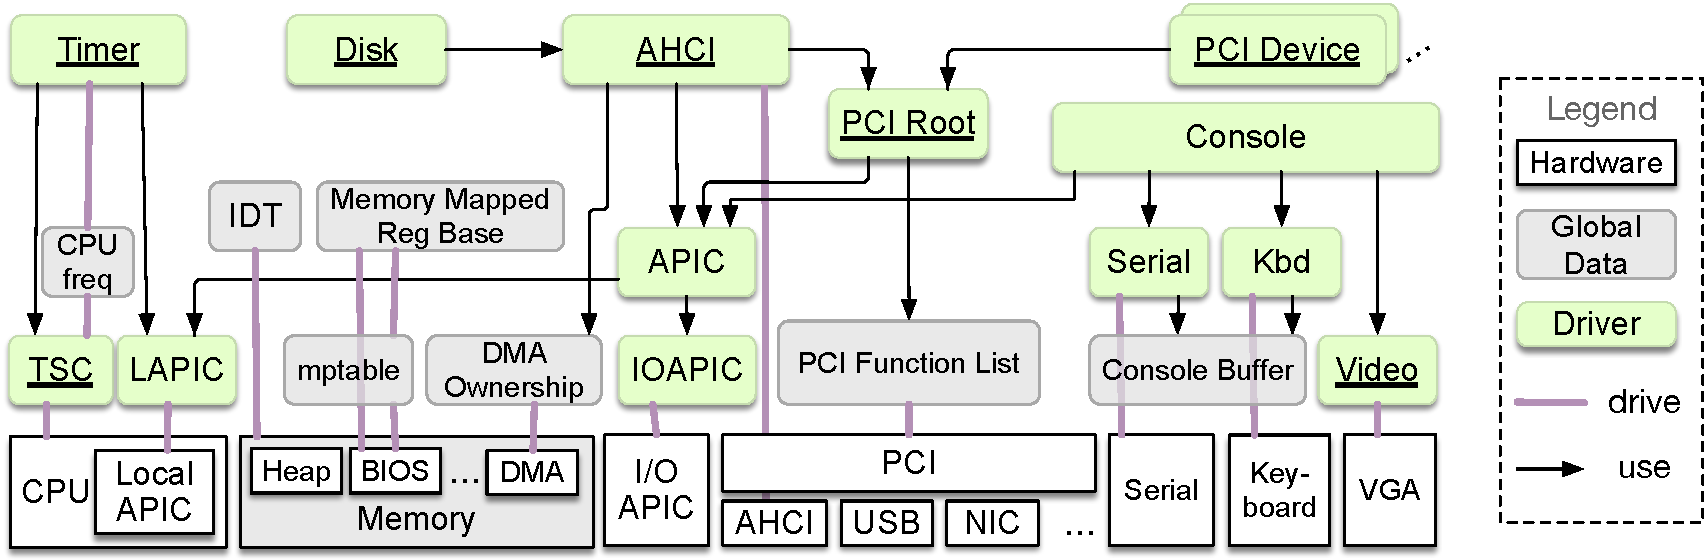
\includegraphics[width=0.95\textwidth]{figs/devices}
\end{center}
\caption{The device driver hierarchy of mCertiKOS}
\label{fig:overview:device}
\end{figure}
%%%%%%%%%%%%%%%%%%%%%%%%%%%%%%%%%%%%%%%%%%%%%%%%%%%%%%%%%%%%%%%%%%%%%%%%%%%%

In this chapter, we present a novel technique on how we can extend
our layer-based technology presented in Chapter \ref{chapter:framework}
to support verification of device drivers and interrupts.
We start from the existing mCertiKOS verified kernel presented in
Chapter \ref{chapter:sequential}. 
The kernel currently runs on the 32 bit x86 architecture.
It provides a multi-processing environment for user-level applications
using separate virtual address spaces. It implements both message
passing and shared memory inter-process communication protocols. As a
hypervisor, it can also boot recent versions of unmodified Linux
operating systems inside a virtual machine.  Unlike large commercial
operating systems like Linux or Unix, the mCertiKOS kernel only implements
a small subset of the POSIX-like API, e.g., process creation and
control, physical and virtual memory management, and
inter-process communication. It does
not implement signals, pipes, {\it etc}. The current file system
implementation in mCertiKOS is not verified. 

Figure~\ref{fig:overview:device} shows the device hierarchy of mCertiKOS. Here
the white boxes represent raw hardware devices; the green boxes denote the
device drivers, and the gray boxes are the data structures used by the drivers.
The purple/black lines show how these device and driver components are related.
Note that the drivers in mCertiKOS are not verified; they are implemented in
about 1,600 lines of C and assembly code and would be considered as part of the
trusted computing base (if they are kept inside the kernel). 

We take mCertiKOS's lowest level machine model, {\it LAsm}, and extend it with
device models. We model devices as finite state transition systems interacting
with the processor and the external environments. Since devices run concurrently
with the processor, parts of the device state change without the processor
explicitly modifying them. Though these ``volatile'' device states can change
nondeterministically, the processor itself only ever observes a ``current''
state when it reads the device data via an explicit I/O operation. The processor
does not, and in fact, {\it cannot} care about any states that the device may
enter between these observed states. Therefore, instead of designing
fine-grained small-step transition systems that model all possible interleaved
executions amongst the processor and devices, our devices simply perform an
atomic big-step transition whenever they are observed, i.e., when there is a
device read/write operation from the CPU.

Next, the machine model needs to be extended with the hardware interrupt
model. The processor responds to an interrupt by temporarily
suspending the current execution and then jumping to another routine
(i.e., an interrupt handler).  Interrupts can be triggered by both
hardware and software. Software interrupts (e.g., exceptions, system
calls) are relatively easy to reason about, since their behaviors are
always deterministic. For example, a page fault exception occurs
whenever the accessed address belongs to an unmapped page or a page
with wrong permission, and a system call is triggered by an explicit
instruction. However, hardware interrupts (IRQs) are unpredictable;
when we execute some code with interrupts turned on, at every
fine-grained processor step, the machine state (e.g., registers and
memory) may undergo significant changes.  Recent work on verified
operating systems (including mCertiKOS) neglects this kind of
reasoning, ignoring one of the largest kernel threat-surfaces
\cite{dscal15,klein2009sel4,Alkassar:VSTTE2010-71}.  Finally, modeling
interrupts is important because it also opens the way toward enabling
interrupts within the kernel.

\ignore{Recent work on verified operating systems (including
  mCertiKOS) avoid this kind of reasoning by either disabling
  interrupts throughout the kernel, or by polling the interrupts at a
  small number of carefully-placed interrupt points
  \cite{dscal15,klein2009sel4,Alkassar:VSTTE2010-71}. Disabling
  interrupts like this leads to a larger interrupt processing
  latency. \josh{also avoiding exceptions in the kernel eliminates
    optimizations like copy-on-write}}

\ignore{ We have developed a framework that supports reasoning of the
  device drivers and the rest of the kernel with potential interrupts
  at arbitrary execution point except in the interrupt handlers. In
  this subsection, we first present our interrupt model at the
  hardware level. Then we show how we gradually refine this low level
  interrupt machine model into the desired higher level one with
  interrupt handlers, where the reasoning of interruptible code can be
  naturally achieved.  }

On top of this lowest-level machine model, each kernel module can be
related to either device drivers (denoted as {\it DD}) or the rest of
the kernel (denoted as {\it K}, representing non-device-related kernel
components).  To introduce, verify, and abstract each such kernel
module into an abstract object with atomic logical primitive
transitions, we need to prove the following isolation properties:
\begin{itemize}
\item For each function in {\it K} or user space, which has interrupts
  turned on, the interrupt must not affect the behavior of the
  function. Although the code can be interrupted at any moment, and
  the control flow transferred to a place outside the function, it
  will eventually return with states (which the function relies upon)
  unchanged.

\item Devices which directly change the memory through Direct Memory
  Access (DMA), do not change any memory that the execution of any
  function in {\it K} depends on.

\item For each interruptible device driver function in {\it DD}, any interrupt
not related to the current device must not change any state related to the
current device.

\item In case that all interrupts related to a device are masked out, no 
interrupts can affect 
the state of the interrupt handler for the device.
\end{itemize}

For a particular fixed set of functions, the proof of the above
properties may not seem hard. However, they have to be proven
repeatedly for all possible combinations of currently introduced sets
of functions and devices. This immediately makes the verification of
an interruptible operating system with device drivers
unscalable. 

\begin{figure}[t]
	\begin{center}
		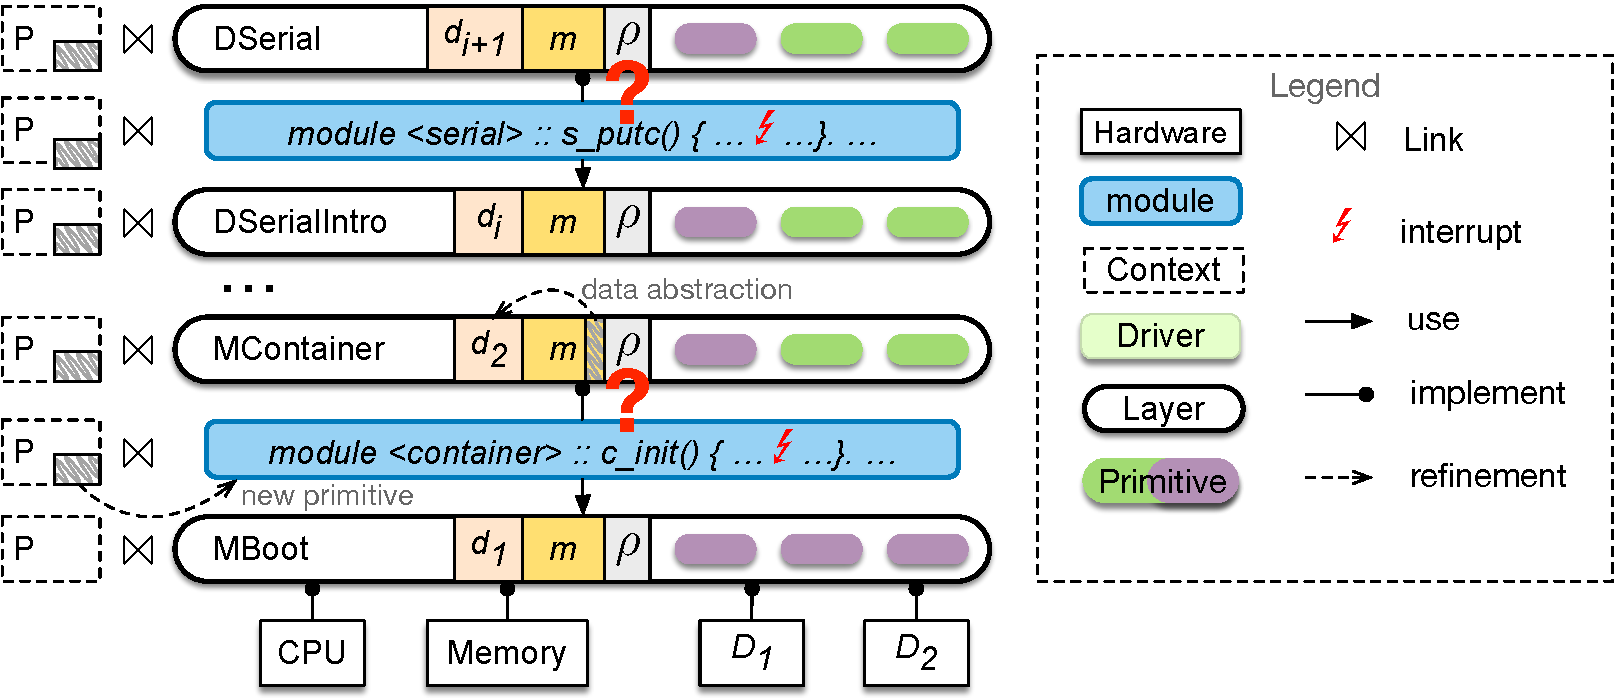
\includegraphics[width=0.95\textwidth]{figs/layer_pre}
	\end{center}
	\caption{Abstraction layers w. interrupts: a failed attempt}
	\label{fig:layer_pre}
\end{figure}

Furthermore, it is not obvious how to apply the techniques presented
in section \ref{chapter:framework}
to handle hardware interrupts. Figure~\ref{fig:layer_pre} shows one
such attempt.  Here, $\textsf{P}$ denotes the kernel/user-level
context code; $\textsf{MBoot}$, $\textsf{MContainer}$,
$\textsf{DSerialIntro}$, and $\textsf{DSerial}$ denote several kernel
and driver layers.  With interrupts turned on in the kernel, it is
immediately unclear how to show contextual refinement among different
layers. For a kernel function like $\textsf{c\_init}$, it cannot be
easily refined into an atomic specification as the code can be
interrupted at any point during the execution by a device interrupt
unless all possible interleavings of interrupts are encoded into the
specification itself. Similarly, for a device driver function like
$\textsf{puts}$, the code can be interrupted at any moment by
interrupts triggered by other devices or the device itself.

\ignore{In our hardware model, the states of CPU (registers and
  memory) and the states of v each device (device registers and
  internal hardware buffers) are strictly isolated. Thus, reasoning
  about their state transitions can be performed separately.}

\ignore{ Each device, together with associated device driver
  primitives and the interrupt handler, are connected with the
  processor in a certain way. The device has pieces of memory that it
  can access, while the device drivers normally have their own data
  stored in memory, e,g, buffers, FIFO queues, {\it etc}. Though they
  seem to be interconnected with the CPU through the memory, if you
  view the combined entity as a whole, it is strictly isolated from
  the entities of other devices, and the rest of the kernel.  The
  purpose of the above detailed properties are used to show that they
  are indeed isolated.  }

In this paper, we propose a systematic way that strictly
enforces isolation among different entities by construction.
Our approach consists of the following two key ideas. 

First, rather than viewing drivers as separate modules that interact
with the CPU via in-memory shared-state, we instead view each driver
as an extended device.  We utilize abstraction layers and contextual
refinement to gradually abstract the memory shared between a device
and its driver into the internal abstract states of a more general
device. Furthermore, we use the same technique to abstract those
driver functions that manipulate these data into the abstract
primitives of a higher level device. After this, our approach ensures
that those abstract states can no longer be accessed by the other
entities, through, e.g., memory reads and writes, but, rather, can
only be manipulated via explicit calls to the device interface. We
repeat these procedures so we can incrementally refine a raw device into
more and more abstract devices by wrapping them with the relevant
device drivers (see Fig.~\ref{fig:driver}). In the rest of the
paper, we call this extended abstract device a {\it device object}, to
distinguish it from the raw hardware device. Note that in our model,
device objects are indeed treated similarly to raw devices, and both
have quite similar interfaces.
% We introduce this name so we can
% refer to the underlying hardware devices unambiguously.

\begin{figure}[t]
	\begin{center}
		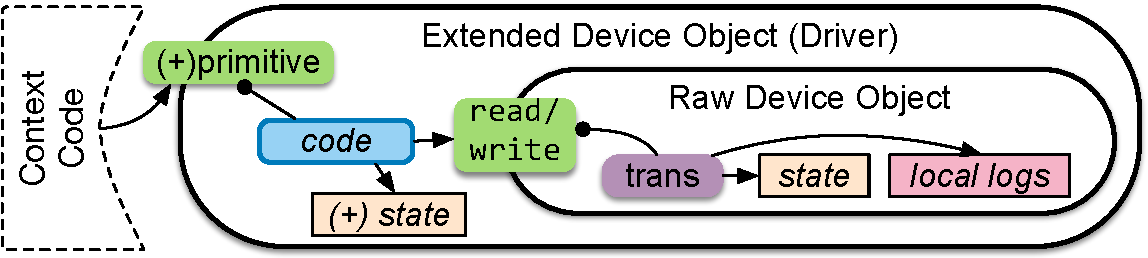
\includegraphics[width=0.75\textwidth]{figs/extends}
	\end{center}
	\caption{The driver as an extended device}
	\label{fig:driver}
\end{figure}

Second, we introduce and verify the interrupt handler for each device
at the lowest machine model, which is not yet suitable for reasoning
about interruptible code. This is possible because, for each device,
we require that either the interrupt be disabled or its corresponding
interrupt line be masked inside the
interrupt handler of the device. Next, we introduce a new abstract
machine with a more abstract interrupt model, that provides strong
isolation properties amongst different device objects and the kernel,
in which any future (context) code with interrupts turned on can be
reasoned about naturally. We prove a strong contextual refinement
property between these two abstract machines: any context code running
on the machine with the abstract interrupt model (overlay) retains an
equivalent behavior when it is running on top of the machine with the
concrete hardware interrupt model (underlay).

\begin{figure}
	\begin{center}
	  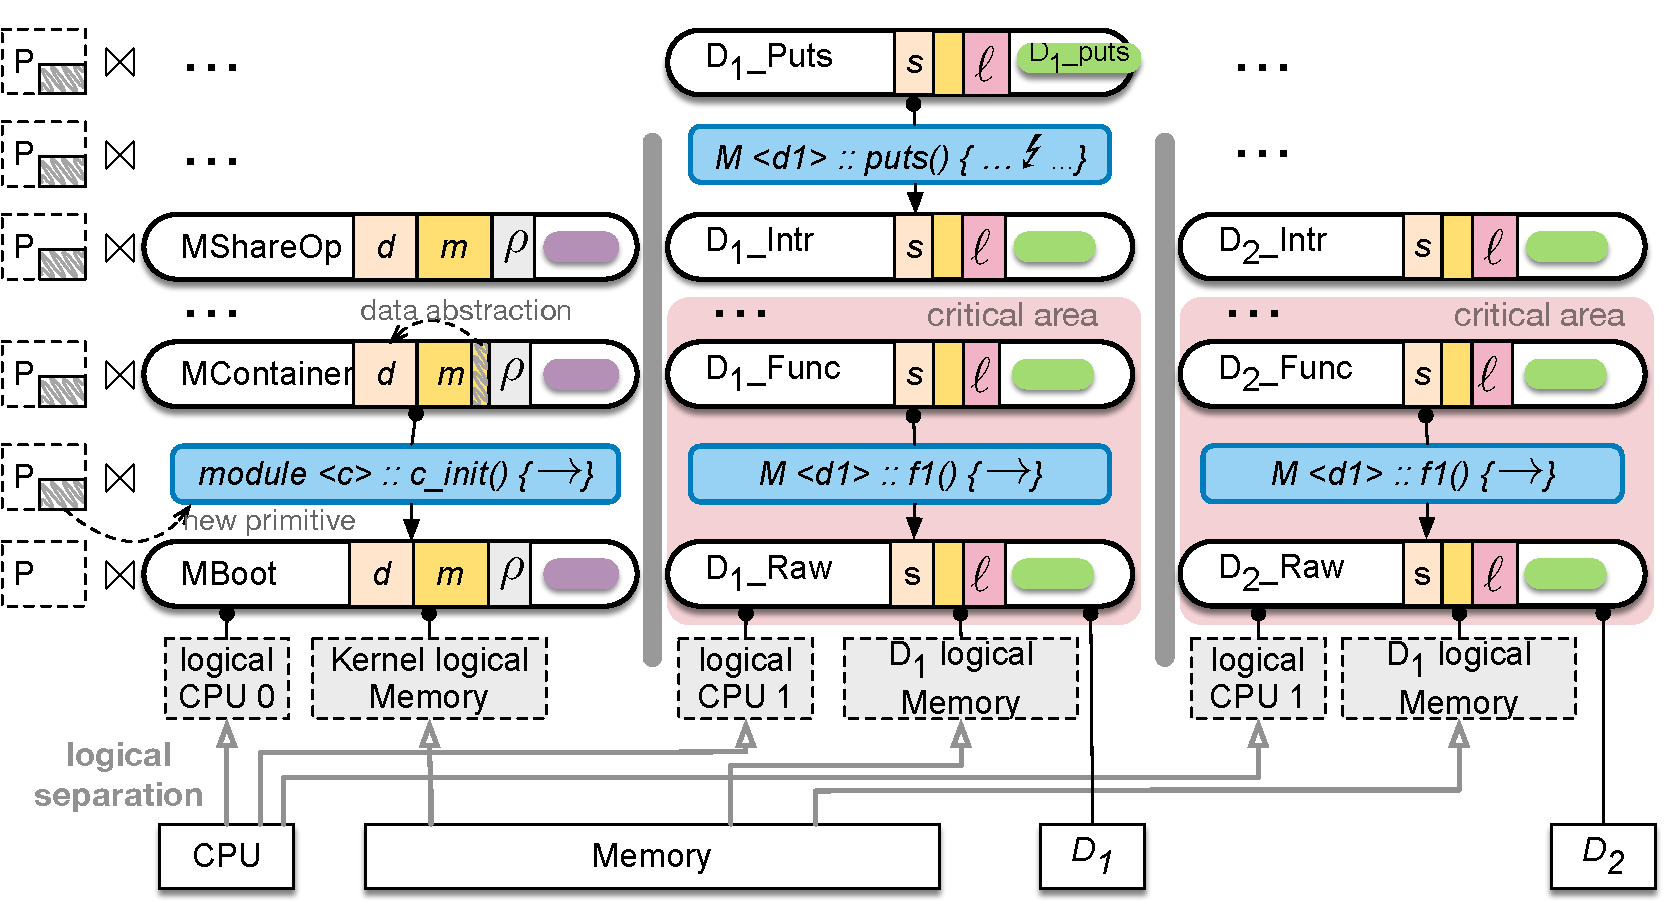
\includegraphics[width=0.90\textwidth]{figs/layer_new}
	\end{center}
	\caption{Building certified abstraction layers with hardware interrupts: our new approach}
	\label{fig:layer_new}
\end{figure}


Figure~\ref{fig:layer_new} shows the layer hierarchy of our
interruptible kernel with device drivers.  We treat the driver code as
if it runs on its own device's ``logical CPU,'' and each logical CPU
operates on its own separate internal states. Thus, the approach
provides a systematic way of assuring isolation among different device
objects (running on its own local logical CPUs) and the rest of the kernel.

On the kernel side (the layer hierarchy on the left hand side of
Fig.~\ref{fig:layer_new}), the contextual refinement is achieved in
the same way as shown in section \ref{chapter:framework} since the hardware interrupts (from
the other logical CPUs with separate states) no longer affect the
execution of any kernel primitive (like $\textsf{c\_init}$), i.e., the
kernel is completely interrupt-unaware.

Similarly, the device driver functions are no longer affected by the
hardware interrupts triggered from other devices.  For each device $D$
running on top of its own logical CPU, we first introduce and verify
part of the driver in the {\em critical area}, i.e., the low-level
device functions that should not be interrupted by the same device,
and the interrupt handler of the device.  Next, we use contextual
refinement to introduce a new layer that has a more abstract interrupt
model. On this layer, we can introduce and verify even interruptible
driver code (e.g., $\textsf{puts}$) while still enforcing strong
isolation and providing a clean interface to the kernel.

The rest of this chapter is organized as follows.
Sec.~\ref{sec:model} defines a formal machine model
extended with raw hardware devices. Sec.~\ref{sec:driver} presents
the device objects, hardware interrupt model, and abstract
interrupt model, and shows how we prove contextual refinement between
the two interrupt models. Sec.~\ref{sec:case_study} shows the Case study
of our verified drivers using the techniques developed in this
chapter, while Sec.~\ref{sec:layers} presents concrete
Coq implementations of certified abstraction layers.
Sections~\ref{sec:lessons} gives an evaluation of our new techniques
and describe the lessons we learned.

\ignore{ At the machine level, the interface between the CPU execution
  and the device state transition is fairly clear. The CPU
  communicates with devices through e.g., I/O instructions, memory
  mapped I/O, while the device interacts with CPU with interrupts,
  Direct Memory Access (DMA), {\it etc}. The executions of the
  programs that do not communicate with devices are isolated to those
  of devices', thus can be reasoned separately.

The very purpose of an operating system is to provide an
abstract device interface to its users. 
Unfortunately, as soon as some device driver code are introduced
in the kernel, it immediately blurs the clean interface between the
operating system and devices. This is because the execution of the
kernel code and transitions of devices are interrelated, i.e., each
side may affect the other one's behaviors, thus making the modular
reasoning extremely complicated. Consider a very simple kernel
function $f$ that copies a small fragments of some device data into some
memory through the device interface, e.g., I/O instructions, memory mapped
I/O, {\it etc}. This preliminary function can
be used in another kernel function to implement a more complex
operation. However, invocation of $f$ affects
both the kernel execution (it modifies memory, thus changes the behavior
of other kernel code depends on this part of memory) and the device
transition (it interacts with devices).  Even worse, some functions may
manipulate several devices simultaneously, e.g., a debug function in a
console driver may write to both the serial port and the display.
This means the kernel execution may affect the transitions of multiple
devices in a rather complex manner. On the other hand, the devices can
also change the behaviors of kernel executions. For the parts of the
kernel with interrupts turned on, devices can interrupt the kernel execution
by an interrupt, force moving the kernel's execution to somewhere else.
When it returns, there is no formal guarantee that the states that the current
execution relies on are not changed by someone else. Furthermore, devices
can also directory change some designated parts of memory through DMA.
The reasoning in this model is complicated as, in theory, any kernel execution
may affect device transitions and any devices may change the behaviors of the
kernel execution. It would be ideal if the two entities are completely isolated
even at very high level of abstractions in the kernel, and the communication
is only done through some clearly specified interfaces that only affects
behaviors of single responsible entity.

In \cite{dscal15}, the authors present a compositional framework to
incrementally build the layers of abstractions
through the notion of contextual refinement, which they apply to
the verification of a practical operating system called mCertiKOS
as a case study.
We extend this framework to build a more powerful framework which
supports a general notion of devices, and compositional verification
of device drivers. One key idea is to broaden the notion of a device.
In our machine model, a ``device'' is no longer limited to a
physical device, but is an abstract representation of one or more
devices together with the functions manipulating those devices.
One observation is that the device drivers,
although could be interconnected in complex ways, are rather isolated from
the rest of operating system (This is not true if the device drivers call sleep or
yield. What should we say about this???). For example, when a serial driver copies
the received serial characters from the serial device into a serial buffer, this
serial buffer stored in memory should be private to the serial driver.
Any good implementation practice of other kernel modules should not directly
access this serial buffer, but through the clean interfaces
provided by the serial driver. In our approach, we view the transitions performed
by the device driver code part of the device transitions. This novel view allows
us to incrementally wrap a physical device with driver code
to build more and more abstract notion of devices, utilizing the idea of
abstraction layers and contextual refinement, while strictly enforcing
isolation between the kernel and ``devices''.

In the case of example above, we utilize the technology presented in \cite{dscal15}, 
to introduce a new abstraction layer on top of the current layer that abstracts
the memory that $f$ manipulates at underlay into an abstract representation
of the same data at overlay. In this framework, abstract states are opaque
to the kernel, and cannot be accessed through regular CPU instructions like
memory operations. The contextual refinement proof between these two abstraction
layers guarantees that the actual information saved in the memory at underlay
and the corresponding abstract representation in the abstract states of overlay
are always related for all possible context code running on the machines,
e.g., more device drivers, any kernel extensions, user programs, {\it etc}.
Then at overlay, we combine this new abstract state with the original device state
to form the state of the new abstract device at overlay, and add $f$ as the
new interface of the new device. Any existing interfaces of original device
at the underlay can be
passed through to the overlay or can be hidden. This can be done for each
device if they do not interfere with each other.
In the case where the newly introduced function interacts with multiple devices,
or multiple devices interfere among each other at the current layer, we merge
these interacting components into a single abstract heterogeneous device.

On the other hand, devices may still affect kernel behaviors, e.g., through
DMA or interrupts. In the case of DMA, we can take similar approach to
abstract the corresponding memory into device abstract states, and incrementally
build more abstract devices through abstraction layers by embarrassing
more and more code that manipulates corresponding devices and memory.
On the other hand,
addressing the issues caused by device interrupts is more complex because,
even in our model above, it is not clear why the device interrupts would
not cause any kernel's states to change. This becomes clear only when 
the interrupt handlers for the devices of interests are fully specified
and verified. At that moment, we have full formal specifications of
behaviors of the device interrupts which can be used to prove the isolation
of kernel execution from device interrupts. In our approach, we perform the
verification of device interrupt handlers as early as possible, and
requires that for these code that run in the very low level of abstraction,
the interrupts are always turned off, e.g., during the execution of device drivers.

Our approach guarantees that any kernel execution would not affect device
transitions except through the well specified interfaces, any device transitions
cannot change the behaviors of kernel execution even in the presence of device
interrupts. Majority of the device driver code in our system are written in C
and verified at the C level, and both the code and the proof are compiled down
to the assembly level through a modified version of the CompCert verified
compiler \cite{dscal15}. With this clean interface enforced by our compositional
framework, reasoning even at a higher level language like C is no longer scary.
During the building of the device hierarchy, the reasoning can be done locally
without worrying about any nondeterministic interference from the original
kernel. We also do not have to change any existing C level proof related to the
kernel in the mCertiKOS, which is completely interrupt-unaware, thanks to this
nice isolation between two entities. (We are gonna insert a figure here to
further illustrate the idea.)

There is still one remaining issue. Majority of our device drivers
are verified at C level. On the other hand, hardware devices run
inherently concurrent to CPU, thus so does our general notion of devices to
the kernel. \newman{Here I am gonna explain our idea of lazily performing
the transitions of each device, logs, and so on. Basically the stuff we do
to determinize the semantics at the C level. I will also talk about
the relation between this deterministic machine to the realistic
non-deterministic machine, and how we can? formally link those together
to illustrate our deterministic machine model is not unrealistic.}

}
     % Overview of Our Approach
\section{Machine Model with Devices}
\label{sec:model}

In this section, we present our machine model, which is based on the Intel x86
architecture. We start from the {\it LAsm} machine model, and extend it
to model devices and interrupts.

Our devices are modeled as finite state transition systems interacting with the
CPU and the external environments. Each read/write (input/output) operation
initiated from the CPU triggers an atomic big-step transition in the
corresponding device.  Device transitions (i.e., $\textsf{trans}$ in
Fig.~\ref{fig:driver}) are affected by two types of interactions, one by the CPU
and another by external events.

\paragraph{Device Transitions caused by the CPU} The CPU may trigger a
device transition through I/O instructions or memory-mapped I/O
operations. These operations can be categorized into the following
two actions:

\begin{definition}[CPU Operation on a Device]
\[
\begin{array}{rll}
\mathcal{O}::= & \textsf{input} ~  n  &~~~~~~\vartriangleright \text{Read value from the register at address $n$} \\
| & \textsf{output}  ~ n ~ v &~~~~~~\vartriangleright \text{Write value $v$ to the register at address $n$}
\end{array}
\]
\end{definition}

For every device, we define an atomic transition function
$\delta^{\textsf{CPU}}$, which takes the current device state $s$ and
a CPU operation $o$, and returns the new state $s'$. Note that
$\delta^{\textsf{CPU}}$ is not a CPU transition, instead, it is strictly a
{\em device transition} triggered by a CPU I/O operation.

\paragraph{Device Transitions caused by External Events}
Device transitions can also be caused by events from the external
environment, such as the keyboard or network, with specific
transitions depending on the kind of event. When modeling these
external events, we take a minimalistic approach: though the devices
can receive all kinds of different external events, we only model
those that change the observable behavior of the device.  Thus, the
events do not map one to one to the transitions in the device hardware but
rather to the CPU observations on the hardware. We model the device
interfaces, not the device internals. The device interface contains
all the information that a programmer can know about its states.
% or interaction with peripheral devices is via the CPU intermediary.
Some example events are:

\begin{definition}[Device External Events] \label{def:eevent}
\[
\begin{array}{rll}
E ::= &  &  \\
 \multicolumn{3}{l}{\vartriangleright \textit{UART device}} \\
 | & \textsf{Recv} ~ (s: \textsf{list} ~ \mathsf{char}) &~~~~~~\vartriangleright \textit{UART receives string s} \\
 | & \textsf{NoSendingCompAck} &~~~~~~\vartriangleright \textit{Sending is not complete} \\
 | & \textsf{SendingCompAck} &~~~~~~\vartriangleright \textit{UART completes the sending} \\
 \multicolumn{3}{l}{\vartriangleright \textit{Keyboard device}} \\
 | & \textsf{KeyPressed} ~ (c: \mathbb{Z}) &~~~~~~\vartriangleright \textit{A specific key is pressed} \\
 | & \textsf{KeyReleased} ~ (c: \mathbb{Z}) &~~~~~~\vartriangleright \textit{A specific key is released} \\
 \multicolumn{3}{l}{\cdots} \\
\end{array}
\]
\end{definition}

External events are unpredictable, as their causes are not controlled by the OS.
We determinize the behavior of each device by parametrizing it with
the set of all possible list of events $\ell^{env}$ that will be processed
sequentially when the CPU performs I/O operations
on this device.
The atomic transition function
$\delta^{\textsf{env}}$ takes an external event $e$ as input and changes the device states
accordingly.

Note that events, even within a single device, can commute. For
example, a serial port serves two roles: to receive user input
and to send program output.  Accordingly, among the events a serial
device can receive are one for the reception of a new input string,
and one signaling that some past output operation has been
completed. Consider a function that first writes to a serial port,
then waits until the write operation is completed by repeatedly
reading some relevant status register. During one of these reads the
user might send new input to the serial port. It would be reasonable
for the device to observe the corresponding {\it \textsf{Recv}} event
during one of the register reads, but doing so would make verifying
the write function unnecessarily complex; not only would a function
need to handle its own logic, but it would also need to handle any
other state transition the device could undergo, even if the result
were not observable in the current function.

\ignore{
\hao{\sout{
One way to mitigate this complexity would be to add invariants to the sequence of
observed events $\ell^{env}$, requiring that some events are in a predefined pattern appears at a point
when the device driver wishes to handle it, but, taken too far, this would make
$\ell^{env}$ contain only a subset of possible input-sequences, thus making the
model unrealistic. Instead, we add rules for how devices observe events.
}} \hao{it is not the correct way}
}

To address this verification challenge, each device keeps a set of
local logs $\vec{\ell} = \{\ell_1, ... \ell_k\}$, each of which is a strict prefix
of $\ell^{env}$.  
\footnote{We have chosen the prefix form over the subset to allow us
determine more easily where the current execution is at on the global
event list.}
The serial device from the example above could
contain two local logs, one for input and one for output.  Then when
$\delta^{\textsf{env}}$ receives an event that does not correspond to
the currently processed action, the event can simply be skipped.
\ignore{
Since the events in separate local logs commute,
when $\delta^{\textsf{env}}$ receives an event that belongs in a local log other than the one
currently being processed, the event can simply be skipped.
}
When a later action observes a part of the device state which is
affected by the event, that action will handle the event. In the
serial port example, we would defer handling the {\it \textsf{Recv}}
event until some process reads from the serial port.

Every raw device provides two I/O primitives: $\texttt{read} ~ n$ and
$\texttt{write} ~ n ~ v$. The $\texttt{read}$ primitive first updates
the device state based on the environmental device transition
$\delta^{\textsf{env}}$ with the next relevant external event in
$\ell^{env}$, then returns a value from the new state, and finally
does the transition $\delta^{\textsf{CPU}}$ triggered by this read
action. The $\texttt{write}$ primitive first triggers the transition
$\delta^{\textsf{env}}$ to update the device state based on the next
relevant external event, then performs the transition
$\delta^{\textsf{CPU}}$ initiated by this write operation.

% In this paper, we use the standard list notations of \textsf{nil},
% \textsf{cons}, \textsf{hd}, and \textsf{tl}.
In the following, the function $\textsf{next}(\ell^{env}, \ell_i)$ finds
the first relevant event $e$ in $\ell^{env}$ that has not yet been
processed with respect to the local log $\ell_i$, and returns the event
$e$ plus a new local log that is synchronized with $\ell^{env}$ up to
the event $e$.

\ignore{
, and define a new list operation:

\begin{small}
	\[ \begin{array}{lrlr}
	\ell_1 - \ell_2 & ::= & \left\{\begin{array}{ll}
	\ell_1 & \textsf{if} ~ \textsf{hd} ~ \ell_1 \neq \textsf{hd} ~ \ell_2 \\
	\textsf{tl} ~ \ell_1 - ~ \textsf{tl} ~ \ell_2 & \textsf{if} ~  \textsf{hd} ~ \ell_1 = \textsf{hd} ~ \ell_2 \\
	\end{array} \right. & \text{(Minus)} \\
	\ignore{
	
	\ell_1 \preceq \ell_2 & \equiv & \ell_1 = \textsf{nil} & (\text{Prefix}) \\
	& | & \textsf{hd} ~ \ell_1 = \textsf{hd} ~ \ell_2 \wedge \textsf{tl} ~ \ell_1 \preceq \textsf{tl} ~ \ell_2 }
	\end{array}
	\] 
\end{small}
}

Now, we define the operational semantics of the set of device primitives
formally. Let $\kappa$ be the function retrieving the value of device register
addressed by $n$, then we have:

\[
	\begin{array}{lr}
	\inferrule{
	(e, \ell'_i) = \textsf{next} (\ell^{env}, \ell_i) \\	
	s' = \delta^{\textsf{env}} (s, e) \\
	res = \kappa(n, s') \\
	s'' = \delta^{\textsf{CPU}} (s', \textsf{input} ~ n) \\
	}{
	\texttt{read} (n, s, \ell_i, \ell^{env}) \defeq (res, s'', \ell'_i) \\
	} & \text{(\texttt{read})} \\
\\
	\inferrule{
	(e, \ell'_i) = \textsf{next} (\ell^{env}, \ell_i) \\	
	s' = \delta^{\textsf{env}} (s, e) \\
	s'' = \delta^{\textsf{CPU}} (s', (\textsf{output} ~ n~ v))
	}{
	\texttt{write} (n, v, s, \ell_i, \ell^{env}) \defeq (s'', \ell'_i) \\
	} & \text{(\texttt{write})} \\
	\end{array}	
\]

\ignore{ \newman{We need to very CAREFULLY explain here that we only
    observe one ``combined'' event in every CPU operation. Then there
    will be the case where there is no external event happened since
    last operation. That's why we have the special NOEVENT event.  We
    have to be careful because this does make the event model
    unrealistic.  Furthermore, we assume that between two operations,
    we would not receive unrelated event (then it cannot be combined
    into one). We can discuss this tomorrow.}  }

Thanks to the local logs, this machine model eliminates much of the
nondeterminism that complicates reasoning about asynchronous systems.
Nonetheless, it accurately models the observable behaviors of real hardware.

Ideally, the global event list should contain a sequence of small atomic
events which gets associated with time when they get triggered. Then the framework
should have some notion of real-time clock that allows us to determine what exact
set of events should be consumed by the next transition based on the current time.
This is out of scope of the current paper. Instead, we allow our transition
to consume a single ``combined'' event (as a list of event). For example, the
``Recv'' event in the Definition \ref{def:eevent} takes a list of characters.
In addition, a device may also consume an ``empty'' event which indicates there
was no event triggered in the real world since the last time we checked $\ell^{env}$.
We parameterize our proof
in a way that it hold for all possible combinations of such combined event
list.

\ignore{
There is a mapping between each $n$ in the $\textsf{input}~n$ /
$\textsf{output}~n~v$ and the state need to be accessed. This mapping is hidden
behind the specification of function $\kappa$ and $\delta^{\textsf{CPU}}$ for
handling output events, and it essentially reflects the interfaces between the
CPU and devices. For most drivers, there are three types of methods to interact
with devices: \textit{port-mapped I/O} and \textit{memory-mapped I/O}.

For the port-mapped I/O, we introduce two primitives: $\textsf{in}~n$ and
$\textsf{out}~n~v$ to branch the port access to the raw device \textsf{read} and
\textsf{write} function. Following the ``logical CPU'' approach in
Sec.~\ref{sec:overview}, we enforce each range of ports only belongs to one
isolated machine, and that guarantees that the device cannot be messed by code
that are not in this driver. Memory-mapped I/O follows the same design. The
memory region that are used to access to one devices is also viewed as the part
of the memory belongs to that device.
}

% In the next section, we show how to extend the
% machine model to reason about interruptible code
% in the kernel.


	 % Device model\includegraphics[scale=1]{../popl15/main.pdf} 
\section{Driver Framework with Interrupts}
\label{sec:driver}

The processor inherently runs in parallel with devices. In Sec.~\ref{sec:model},
we have presented a machine model representing this level of concurrency. On top
of this machine model, we build certified abstraction layers introducing more
and more driver code. At each abstraction layer, our model enforces systematic
isolation among the different device objects and the rest of the kernel, so that
interaction with one device object does not affect the states of other device
objects nor the rest of the kernel. Thus, isolation properties are satisfied by
construction. This dramatically simplifies our reasoning by allowing us, at any
given time, to focus on only the device objects that are currently interacted
with.

In this section, we define the device object more formally; then we show how to
incorporate interrupts into our model while still following our isolation
policy.

\subsection{Device Objects}

\begin{figure}
\begin{center}
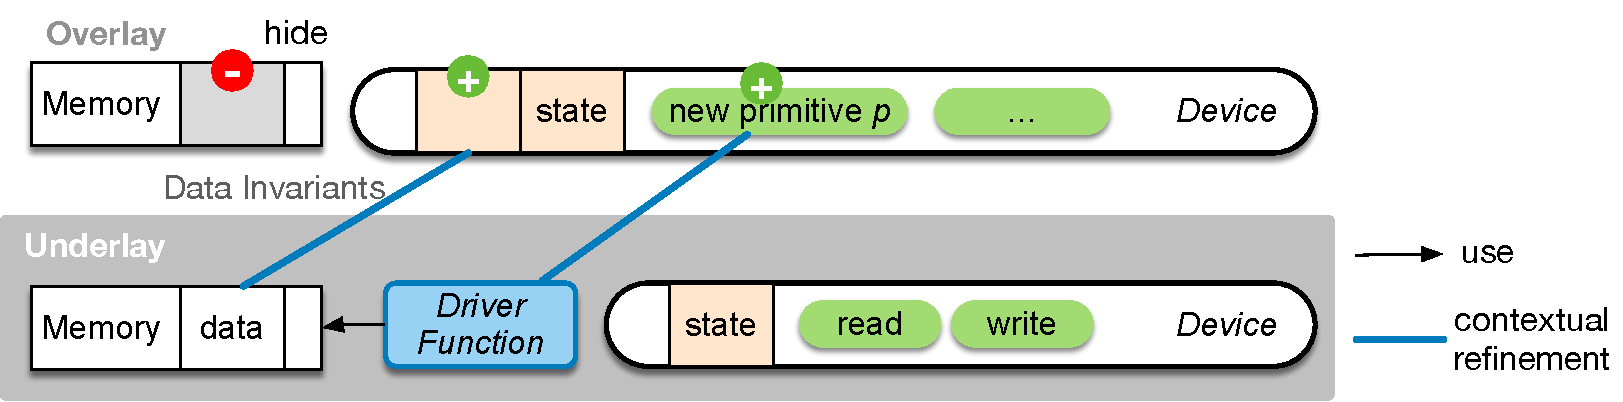
\includegraphics[width=0.95\textwidth]{figs/object}
\end{center}
\caption{Layer-based contextual refinement of the device object}
\label{fig:spec:object}
\end{figure}

\ignore{ In Chapter \ref{sec:model}, we talked about using the local and global
	log to reason about this concurrency. However, when it comes to the driver
	level, things are different. Drivers' code is executing inside CPU, but it may
	trigger device transition. Moreover, a driver usually has its own data, e.g.
	buffer, FIFO queue, which is stored in the memory. That means, while the memory
	of a driver is being changed, its device states may change at the same time. For
	example, when a driver fetching a data unit from the buffer, it may be
	interrupted by its interrupt handler, which tries to adding a unit into the
	buffer. Usually we simply disable the interrupt or mask that interrupt line
	during the fetching operation to rule out this race condition. However, we have
	to prove that the whole context, i.e. all possible program in the universe,
	disable their interrupt before touching these data. If we just mask the
	interrupt line, we have to prove all other interrupt handler in the context will
	not touch these data too. It is an impossible job. }

A {\it device object} is a logical abstraction containing a hardware device plus
its related drivers. Each device object consists of a set of abstract states,
abstracting the private states of the device (e.g., device registers, driver
private memory); and a set of primitives, abstracting the module interface. The
abstract states are private to the device object, and can only be manipulated by
explicit calls to the device object's primitives. This is achieved by
establishing a contextual refinement relation from the concrete memory and
device function implementation to the abstract state and primitives. As shown in
Fig.~\ref{fig:spec:object}, we follow the layer-based methodology introduced in
Chapter \ref{chapter:framework}
and utilize the CompCert memory permissions~\cite{leroy08} to hide the relevant
memory at overlay, which prevents the context code from accessing the object's
private data. These logical permissions do not correspond to any physical
protection mechanism, but are used to ensure that the abstract machine at
overlay gets stuck if any code tries to directly access this portion of data.
The safety proof of our entire operating system (the kernel never gets stuck)
guarantees that such a situation never happens.  The set of driver functions at
underlay, which manipulate the memory that will be abstracted away at overlay,
are themselves abstracted into the set of device primitives at the overlay (see
Fig.~\ref{fig:spec:object}).

For example, the console buffer is implemented as a circular buffer in our
console driver.  The concrete implementations of the buffer operators ({\it
	cb\_read} and {\it cb\_write}) directly manipulate the concrete circular
buffer in memory. At a higher layer, in our abstract console device object, the
logical buffer is represented as a list, and the primitives are specified
directly over this abstract list, i.e., the {\it cb\_read} simply returns the
head element in the list, while {\it cb\_write} adds the new element to the end
of the list, discarding a single head element if the size of the list exceeds
its limit.  The contextual refinement relation between the two layers ensures
that any code running on top of the more abstract overlay exhibits behavior
equivalent to running on top of the underlay.

The primitives at the underlay can be passed through to the overlay, or hidden
if they are no longer needed.  For example, once the primitive {\it
	ahci\_transfer} is introduced at the overlay, the underlay primitives {\it
	ahci\_read} and {\it ahci\_write}, used to implement {\it ahci\_transfer}, are
hidden. This facilitates the invariant proofs as stronger invariants can be
introduced at higher layers, which could otherwise be violated by the
lower-level primitives.

This kind of abstraction does not necessarily have to include any code, and sometimes
are achieved already at the raw device level. For example, some part of memory
may be designated to the hardware device to set up the direct memory access (DMA)
to allow the device directly read from or write to the main memory without
going through the main CPU. In this case, the part of memory designated for DMA
can also be abstracted into the device's internal abstract states through the
contextual refinement.

\ignore{

Instead of treating a driver as part of the kernel, we treat it as an extension
of the device. As shown in Figure x \hao{need a figure}, the driver just
encapsulates the original device and includes additional functions. A driver is
the abstraction of a device, which means it is still a device, and the memory
owns by it becomes part of the internal states. Even though, the new device
still follows the rule of a general device: kernel execution and the transitions
of devices are strictly isolated, thus their reasoning can be easily separated
and composed.

If a memory block needs to be added into the internal states, we first hide it
in the memory and then add it into the volatile state of the extended device.
$s^{(+)} = (d_1: T_1, d_2: T_2, ...)$. \hao{do we need to explain more here?}
After that, we add the basic primitives to access it. In this way, the context
can only operates the data through these primitives. Moreover, only the code
belongs to this device can invoke primitives of this device. That naturally
gives the isolation of interrupt handlers between devices.

After the device becomes more abstract, we can hide the unnecessary primitives
and only expose the higher-level ones. For example, if \texttt{ahci\_transfer}
is already introduced, we will no longer need \texttt{ahci\_readl} and
\texttt{ahci\_writel}. }

\paragraph{Combining Device Objects}

At a certain abstraction layer, some drivers, or more generally, system
services, may interact with multiple device objects, by, e.g., transferring data
between two devices, or broadcasting messages to multiple devices.  At this
stage, such devices are no longer totally isolated, but are synchronized through
hardware or software mechanisms.  This does not fit directly into our model
providing systematic isolation among different device objects and the rest of
the kernel.

In the above scenario, we introduce at the overlay a single heterogeneous device
object, which combines the device objects from the underlay via the newly
introduced functions. The abstract machine at overlay thereby provides
systematic isolation between the new abstract device object and the rest of the
kernel. The internal states and local logs of the combined device object are the
disjoint union of the relevant objects at underlay, while the functions that
manipulate multiple device objects at underlay become primitives of the new
device object, operating on a wider range of internal states, at overlay. As in
all device objects, existing primitives can be either passed through to this new
device, or hidden.


\subsection{Interrupts}

We now show how to adapt the interrupts into our setting.  We first present our
interrupt model at the hardware level, where the interrupt transitions are
separately defined for the CPU, the interrupt controllers (IC), and the devices.
At this low level we lack the full behaviors of interrupt handlers, so all the
primitives verified at this machine level have the precondition that interrupts
are disabled or the corresponding interrupt lines are masked. A special flag
$\mathsf{critical}$ is defined in the abstract state of each device to make sure
that every such low level primitives have precondition of $\mathsf{critical}$ 
being $\mathsf{true}$ to enter the critical section for accessing the data
shared between the primitives and the interrupt handler
of the device.  On top of this hardware abstraction layer, we
incrementally introduce and verify interrupt handlers for each device through
abstraction layers.  Above a certain abstraction layer, we have full behaviors
of the interrupt handlers, so we introduce a new abstraction layer with an
abstract interrupt model, where an interrupt only changes the state of the
device object that triggered it.  This makes the interrupt completely
transparent to the CPU, the IC, and other devices; thus, guaranteeing our
desired isolation properties.  We prove the strong contextual refinement
property between these two abstraction layers to ensure that any context program
running on top of the overlay retains behavior equivalent to running atop the
underlay. Starting from the abstraction layer with the abstract interrupt model,
we support verification of any code with interrupts enabled.

%%%%%%%%%%%%%%%%%%%%%%%%%%%%%%%%%%%%%%%%%%%%%%%%%%%%%%%%%%%%%%%%%%%%%%%%%%%%
\begin{figure}[t]
	\begin{center}
		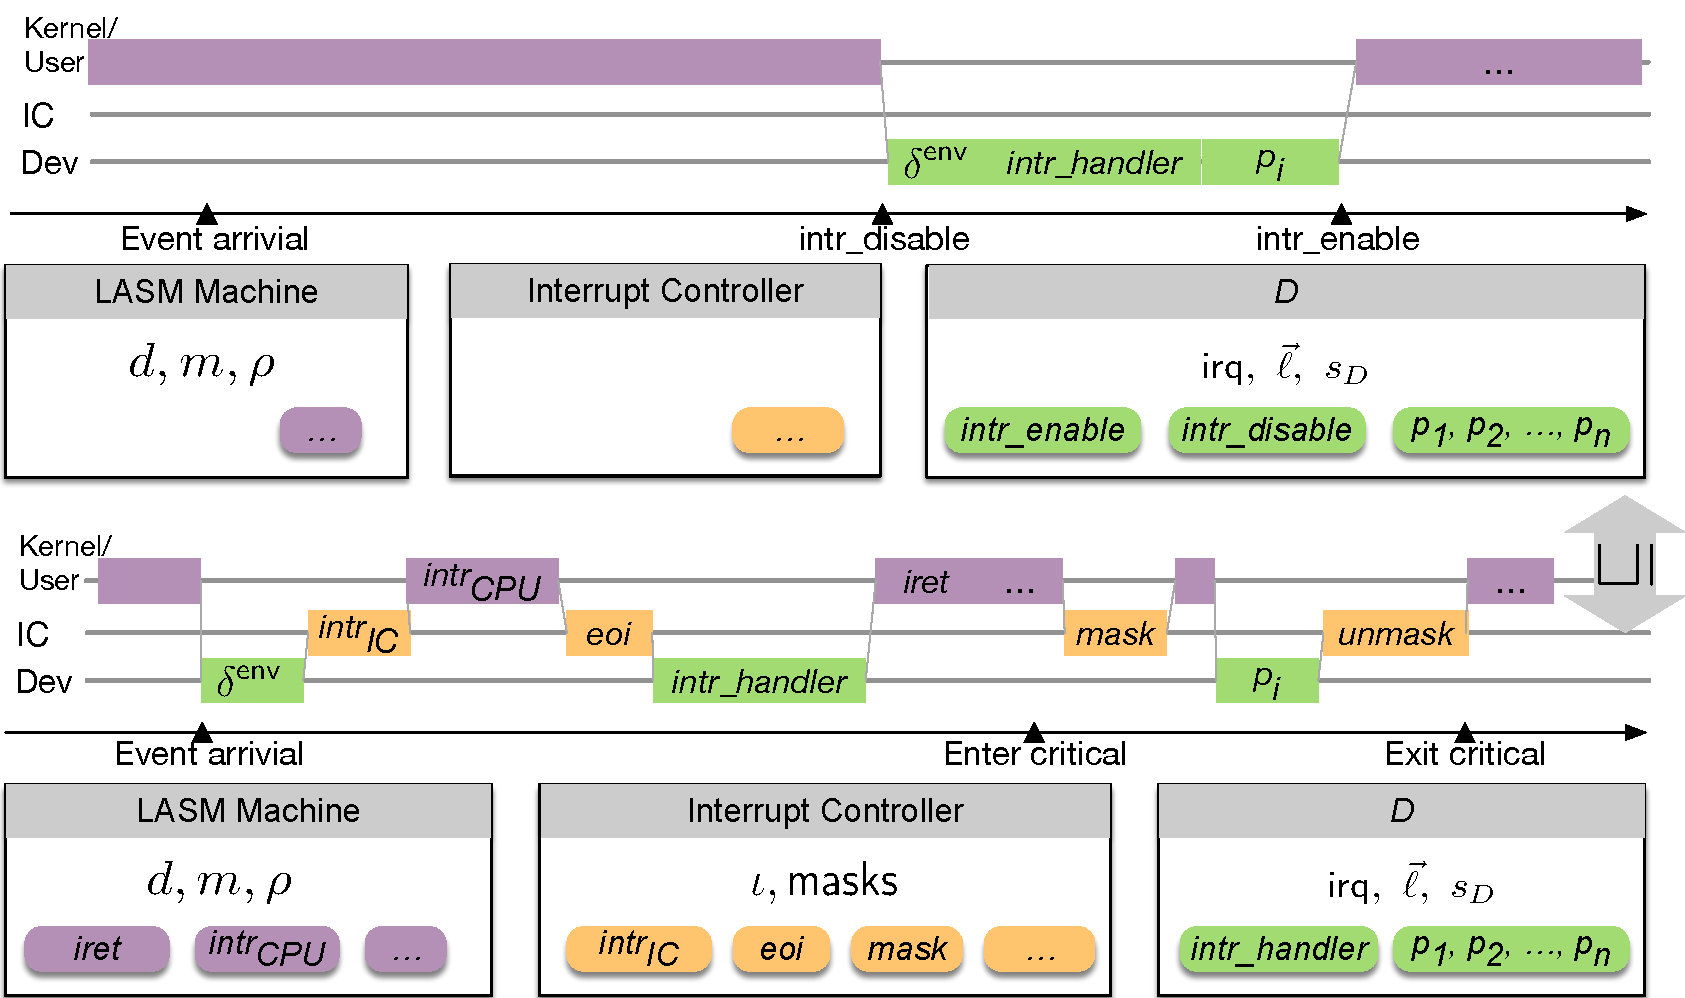
\includegraphics[scale=0.4]{figs/interrupt}
	\end{center}
	\caption{The hardware interrupt model (bottom), the
          abstract interrupt model (top), and the contextual
          refinement between these two models.}
	\label{fig:interrupt}
\end{figure}
%%%%%%%%%%%%%%%%%%%%%%%%%%%%%%%%%%%%%%%%%%%%%%%%%%%%%%%%%%%%%%%%%%%%%%%%%%%%

The entities involved in any given interrupts are categorized into three parties
(shown in the bottom half of Fig.~\ref{fig:interrupt}).  If a device transition
(e.g., from the device $D$ in Fig.~\ref{fig:interrupt}) triggers an interrupt,
it gets sent to the IC.  The IC multiplexes several interrupt lines onto the CPU
(i.e., the \textit{LAsm} machine in Fig.~\ref{fig:interrupt}), with the ability
to mask and unmask each interrupt line. At each transition, the IC selects the
pending unmasked interrupt with the highest priority and forwards it to the CPU.
When the CPU receives an interrupt signal, it first checks whether interrupts
are enabled on that CPU, and, if so, saves the current context and jumps to the
corresponding entry in the interrupt descriptor table (IDT). If interrupts are
turned off, the interrupt signal is ignored. Thus, an interrupt involves at most
three consecutive transitions: the device, the IC, and the CPU.  These three
transitions seem inter-related, and isolation among the three entities is
non-obvious.  In our approach, we first develop a low level hardware interrupt
model that separately defines the set of interrupt related operations.  Then
these three disconnected components are united at some higher level abstract
machine model after we have verified all the interrupt handlers.


\subsubsection{Interrupt Transition for Devices}

As described in Sec.~\ref{sec:model}, every raw device has its own
transition function $\delta^{\textsf{env}}$ specifying how it reacts
to the external events. When a particular transition triggers an
interrupt (e.g., see the event arrival and the green box
$\delta^{\textsf{env}}$ along the {\tt Dev} line in the bottom half of
Fig.~\ref{fig:interrupt}), the device marks an interrupt request bit
({\it irq}) in its internal state.


\subsubsection{Interrupt Transition for IC}
When the IC receives an interrupt signal (e.g., see the orange box
$\texttt{intr}_{\textsf{IC}}$ along the {\tt IC} line in
Fig.~\ref{fig:interrupt}), it first checks whether the particular
interrupt line is masked, and if so, it ignores the interrupt; if not,
then the IC marks the corresponding interrupt line.  The
transition rules are defined in Fig.~\ref{fig:interrupt-ic}.  Here,
$N_D$ is the corresponding interrupt line number of the device $D$
which triggered the interrupt; it is fixed by the hardware connection,
and is mapped to $\textsf{IRQ} ~ n$ by the configuration of the IC;
the $\iota$ field of $s_{\textsf{IC}}$ indicates which $\textsf{IRQ}$
number is raised; we use $\emptyset$ to indicate that there is no
raised interrupt. After the CPU performs its initial interrupt
transition, the IC would receive the End Of Interrupt (EOI) signal
(e.g., see the orange box $\texttt{eoi}$ along the {\tt IC} line in
Fig.~\ref{fig:interrupt}), it clears the raised mark on the interrupt
line.  The IC also has two primitives {\it mask} and {\it unmask},
which set the $s_{\textsf{ic}}.\textsf{masks}[N_D]$ of the interrupt
line number $N_D$ to \textsf{Masked} and \textsf{Unmasked}
respectively.


\ignore{ \hao{We do not need to extract the interrupt event. We can always let
		devices make their transition, and mark an interrupt request bit. At the
		interrupt handler level, after each transition, we check this bit. If it says
		the last transition triggered an interrupt we invoke the IC's \texttt{intr}
		primitive and check if the interrupt line is masked. If it is not, we ask CPU to
		invoke interrupt handler. When we scan the log, it indicates that the interrupt
		in the CPU is enabled. Thus, the interrupt handler will first call \texttt{eoi}
		to recover the IC. Since interrupt handler is also transparent to IC, we can
		call it in our interrupt handler. In this way, interrupt handler is a special
		device which has no local log. The reason is that every operation on it is in a
		pair (\texttt{intr}, \texttt{eoi})} }


%%%%%%%%%%%%%%%%%%%%%%%%%%%%%%%%%%%%%%%%%%%%%%%%%%%%%%%%%%%%%%%%%%%%%%%%%%%%
\begin{figure}[t]
	\begin{center}
\[
\begin{array}{cr}
	\inferrule{
			s_{\textsf{ic}}.\textsf{masks}[N_D] = \textsf{Masked} \\
			s_{\textsf{ic}}.\textsf{irqs}[N_D] = n
	}{
		\texttt{intr}_{\textsf{IC}} (s_{\textsf{ic}}, N_D) \defeq (s_{\textsf{ic}}, \emptyset) } & \text{($\texttt{intr}^{m}_{\textsf{IC}}$)} \\[5ex]

\inferrule{
		s_{\textsf{ic}}.\textsf{masks}[N_D] = \textsf{Unmasked} \\
		s_{\textsf{ic}}.\textsf{irqs}[N_D] = n \\	
		s_{\textsf{ic}}.\iota = \emptyset 
	}{
  \texttt{intr}_{\textsf{IC}} (s_{\textsf{ic}}, N_D) \defeq
           (s_{\textsf{ic}}[\iota \leftarrow \textsf{n}], \textsf{IRQ}~n)
} & \text{($\texttt{intr}^{u}_{\textsf{IC}}$)} \\[5ex]

\inferrule{
	}{	
		\texttt{eoi} (s_{\textsf{ic}}) \defeq s_{\textsf{ic}}[\iota \leftarrow \emptyset]
	} & \text{($\texttt{eoi}$)} 
\end{array}
\]
	\end{center}
	\caption{Interrupt transition for the IC}
	\label{fig:interrupt-ic}
\end{figure}
%%%%%%%%%%%%%%%%%%%%%%%%%%%%%%%%%%%%%%%%%%%%%%%%%%%%%%%%%%%%%%%%%%%%%%%%%%%%


\subsubsection{Interrupt Transition for the CPU} As soon as the IC marks 
an interrupt line as raised, the CPU will perform its own interrupt
transition (e.g., see the purple box $\texttt{intr}_{\textsf{CPU}}$
along the {\tt Kernel/User} line in Fig.~\ref{fig:interrupt}).  Let
$\rho$ represent the register set, and $d$ be the
logical abstract states in the machine model, then the interrupt
transition of a CPU is shown in Fig.~\ref{fig:interrupt-cpu}.

%%%%%%%%%%%%%%%%%%%%%%%%%%%%%%%%%%%%%%%%%%%%%%%%%%%%%%%%%%%%%%%%%%%%%%%%%%%%
\begin{figure}[t]
	\begin{center}
	\[
	\begin{array}{cr}
	\inferrule{
		\rho[\textsf{EFLAGS}.\textsf{if}] = \textsf{Disabled} 
	}{
	\texttt{intr}_{\textsf{CPU}} (d, \rho, \textsf{IRQ}~n) \defeq (d, \rho)
	} & \text{($\texttt{intr}^{d}_{\textsf{CPU}}$)} \\[5ex]

	\inferrule{
		\rho[\textsf{EFLAGS}.\textsf{if}] = \textsf{Enabled} \\
       		d' = d[\textsf{isr} \leftarrow \textsf{true}] \\
		\textsf{tfs'} = \texttt{save\_context}(d'[\textsf{tfs}], \rho)\\\\
		d'' = d'[\textsf{tfs} \leftarrow \textsf{tfs'}] \\
                		\textsf{IDT}[n] = p \\
		\rho' = \rho[\textsf{EIP} \leftarrow p][\textsf{EFLAGS}.\textsf{if} \leftarrow \textsf{Disabled}]
	}{
	\texttt{intr}_{\textsf{CPU}} (d, \rho, \textsf{IRQ}~n) \defeq (d'', \rho') 
	} & \text{($\texttt{intr}^{e}_{\textsf{CPU}}$)}  \\[5ex]

	\inferrule{
		(\textsf{tfs'}, \rho') = \texttt{restore\_context}(d[\textsf{tfs}]) \\
		d' = d[\textsf{isr} \leftarrow \textsf{false}][\textsf{tfs} \leftarrow \textsf{tfs'}]
	}{
	\texttt{iret} (d, \rho) \defeq (d', \rho') 
} & \text{($\texttt{iret}$)} 
\end{array}
\]
	\end{center}
	\caption{Interrupt transition for the CPU}
	\label{fig:interrupt-cpu}
\end{figure}
%%%%%%%%%%%%%%%%%%%%%%%%%%%%%%%%%%%%%%%%%%%%%%%%%%%%%%%%%%%%%%%%%%%%%%%%%%%%

We use $\textsf{EFLAGS.if}$ to represent the interrupt flag
bit in the $\textsf{EFLAGS}$ register.  If interrupts are disabled
inside the CPU, the $\texttt{intr}_{\textsf{CPU}}$ primitive is totally
transparent. Otherwise, it first changes the logical \texttt{isr}
state to \texttt{true}, saves the current context into the end of the
trap frame list ($d'[\texttt{tfs}]$), and jumps to the corresponding IDT
entry. Here \texttt{isr} indicates whether the current machine
execution is in the interrupt handling mode; the \texttt{save\_context}
function models the hardware behavior of saving the current context into
the abstract state ($d'[\texttt{tfs}]$), which corresponds to the concrete
stack frames in the memory (abstracted in layers below). 

The primitive \texttt{iret} is the counterpart of
$\texttt{intr}_{\textsf{CPU}}$, and models the behavior of CPU when
the interrupt handler returns.  It restores $\textsf{EFLAGS}$
(including the old interrupt flag bit) from the context and thus also
re-enable interrupts. The \texttt{restore\_context} function
models the hardware behavior of restoring the current context
from the abstract state ($d[\texttt{tfs}]$).

\begin{lemma} \label{lemma:context}
  The function \texttt{restore\_context} is a left inverse of
  the function \texttt{save\_context}. 
  
  \[\begin{array}{c}
		\inferrule{
			\textsf{tfs}' = \texttt{save\_context}(d[\textsf{tfs}], \rho) \\\\ 
			(d', m', \rho') = f (d[\textsf{tfs}\leftarrow\textsf{tfs}'], m, \rho) \\\\
			d[\textsf{tfs}] = d'[\textsf{tfs}] \\\
			(\textsf{tfs}'', \rho'') = \textsf{restore\_context}(d'[\textsf{tfs}])
		}{
			\textsf{tfs} = \textsf{tfs}'' \wedge \rho = \rho '' 
		} 
  \end{array}\]
  
  \ignore{
  $(\texttt{tfs}, \rho) = \textsf{restore\_context}(\texttt{save\_context}(\textsf{tfs}, \rho))$
  }
\end{lemma}

The CPU also has two primitives {\it sti} and {\it cli}, which
set the $\textsf{EFLAGS}.\textsf{if}$ bit to \textsf{Enabled}
and \textsf{Disabled} respectively.

% In the bottom half of Figure~\ref{fig:interrupt}


%%%%%%%%%%%%%%%%%%%%%%%%%%%%%%%%%%%%%%%%%%%%%%%%%%%%%%%%%%%%%%%%%%%%%%%%%%%%
\begin{figure}[t]
	\[\begin{array}{lc}
\multicolumn{2}{l}{\textsc{DisableNoIntr:} ~ \text{Disable with no unhandled interrupt}} \\[1ex]
& \inferrule{
		(e, \ell'_i) = \textsf{next} (\ell^{env}, \ell_i) \\	
		s_{\textsf{tmp}} = \delta^{\textsf{env}} (s, e) \\\\
		s_{\textsf{tmp}}.irq = \textsf{false} \\
		s' = s[\textsf{critical} \leftarrow \textsf{true}] 
	}{
	\texttt{intr\_disable} (s, \ell_i, \ell^{env}) \defeq (s', \ell_i) 
} \\[5ex]

\multicolumn{2}{l}{\textsc{DisableIntr:} ~ \text{Disable with unhandled interrupts}} \\[1ex]
& \inferrule{
		(e,\ell'_i) = \textsf{next} (\ell^{env}, \ell_i) \\	
		s' = \delta^{\textsf{env}} (s, e) \\\\
		s'.irq = \textsf{true} \\
		(s'', \ell_i'') = \texttt{intr\_handler} (s', \ell'_i, \ell^{env}) \\
		(s''', \ell_i''') = \texttt{intr\_disable} (s'', \ell''_i, \ell^{env}) 
	}{
	\texttt{intr\_disable} (s, \ell_i, \ell^{env}) \defeq (s''', \ell_i''') 
} \\[5ex]

\multicolumn{2}{l}{\textsc{EnableNoIntr:}~\text{Enable with no raised interrupt}}\\[1ex]
& \inferrule{
	s.irq = \textsf{false} \\
	s' = s[\textsf{critical} \leftarrow \textsf{false}] 
}{
\texttt{intr\_enable} (s, \ell_i, \ell^{env}) \defeq (s', \ell_i) 
}\\[5ex]

\multicolumn{2}{l}{\textsc{EnableIntr:} ~ \text{Enable with raised interrupts}}\\[1ex]
& \inferrule{
	s.irq = \textsf{true} \\
	(s', \ell'_i) = \texttt{intr\_handler} (s, \ell_i, \ell^{env}) \\
	(s'', \ell_i'') = \texttt{intr\_enable}(s', \ell_i', \ell^{env}) 
}{
	\texttt{intr\_enable} (s, \ell_i, \ell^{env}) \defeq (s'', \ell_i'') 
}
\end{array}\]
\caption{Transition rules for {\it intr\_disable} and {\it intr\_enable}}
	\label{fig:intr-transition}
\end{figure}

%%%%%%%%%%%%%%%%%%%%%%%%%%%%%%%%%%%%%%%%%%%%%%%%%%%%%%%%%%%%%%%%%%%%%%%%%%%%

\subsubsection{Abstract Interrupt Model} \label{sec:interrupt}

The low-level machine model, we just described, is not suitable for
reasoning about interrupts, since each of the three entities has its
own disconnected view.  For instance, when the CPU jumps to an IDT
entry, it is unaware of the behavior of the corresponding interrupt
handler, and when the IC sends an interrupt signal to the CPU, it does
not know whether the interrupt will be handled or not. We would like
to formally connect these three different views to derive a nice
machine model that is suitable for reasoning about the end-to-end
behavior of interrupts, i.e., an interrupt triggered by a device only
modifies the particular device's internal states, and is transparent
to the CPU, the IC, and other devices.  To achieve this, we need a
model of the full behavior of the interrupt handler for each device.

Starting from the above hardware interrupt model, we incrementally extend a raw
device by wrapping it with driver code related to the interrupt handler, until
we have fully verified the interrupt handler for the device.  Each device has
exactly one interrupt handler, which, by our isolation policy, only modifies
the internal states of its particular device (Lemma~\ref{lemma:intr-handler}),
and cannot itself be interrupted by the same device.

\begin{lemma} \label{lemma:intr-handler}
The interrupt handler (\texttt{intr\_handler}) of device $D$ can only observe
and modify the abstract states of $D$.
%\[
%\begin{array}{c}
%	\inferrule{
%		d = (s_1, s_2, ..., s_D, ...) \\
%		d' = (s'_1, s'_2, ..., s'_D, ...) \\
%		s_D = s'_D \\
%	}{
%		\texttt{intr\_handler}_D (d, \ell_i, \ell^{env}) \defeq \texttt{intr\_handler}_D (d', \ell_i, \ell^{env}) 
%	}\\[5ex]
%	\inferrule{
%		d = (s_1, s_2, ..., s_D, ...) \\
%		d' = (s'_1, s'_2, ..., s'_D, ...) \\
%		(d, \ell'_i) = \texttt{intr\_handler}_D (d, \ell_i, \ell^{env}) \\
%		1 \le j \le |d| \\
%		j \neq D
%	}{
%		 s_j = s'_j \\
%	}
%	\end{array}
%\]
\end{lemma}

At this stage, we have the formal specification of the interrupt
handler for a device.  Next, through contextual refinement, we
encapsulate the behaviors of interrupts into two primitives {\it
  intr\_enable} and {\it intr\_disable} at overlay for the device,
which, as shown in the top half of Fig.~\ref{fig:interrupt}, render
interrupts transparent to the CPU and the IC.  The precise
transition rules are given in Fig.~\ref{fig:intr-transition}. 
Here, the $\textsf{next}$
function, as defined at the end of Sec.~\ref{sec:model}, returns the
next relevant event in $\ell^{env}$ and a new local log synchronized
with $\ell^{env}$ up to the returned event. Before,
the states on whether each device's interrupt line is masked or not
were part of the IC devices. Following our isolation policy, in the
new abstract interrupt model, we introduce a new abstract state
$\textsf{critical}$ in the device itself to indicate whether the particular
interrupt is masked. When $\textsf{critical}$ is $\textsf{true}$,
it indicates that the interrupt line for the device is masked, thus
the execution can enter the critical sections to read and write the device
internal states, and {\it vice versa}. Recall that all the low level
primitives (ones introduced before the interrupt handler) of the device
have the precondition of $\textsf{critical}$ to be 
$\textsf{true}$ to enter the critical section.

The {\it intr\_disable} primitive first synchronizes the device state
with the previously unhandled interrupts then sets interrupt as
disabled.  It performs the synchronization by scanning the log from
the last place {\it intr\_enable} was called, until we hit the first
event that did not trigger any interrupt.  This ensures that
subsequent observations on the device (in the abstract model) will be
consistent with those performed under the hardware interrupt model.
Note that {\it intr\_disable} is defined recursively: it performs the
environment transition $\delta^{\textsf{env}}$ on each event until we
hit an event that does not trigger interrupts (i.e., the
\textsc{DisableNoIntr} case); the $s_{\textsf{tmp}}$ state should be 
discarded since the device
transition stops at the point where the last unhandled interrupt is
handled.

The {\it intr\_enable} primitive discharges any raised interrupts,
then sets interrupt as enabled. This models the physical machine
behavior, wherein interrupts (which can occur while interrupts are
disabled) get delayed until interrupts are re-enabled. This causes the
OS to immediately jump to the interrupt handler after re-enabling
interrupts. This repeats until the device no longer attempts to
trigger an interrupt within the interrupt handler, and normal
execution can continue.

With these two new primitives, the CPU transition in the abstract
interrupt model can be completely oblivious of the device
transitions. For example, in the top half of Fig.~\ref{fig:interrupt},
the purple box along the {\tt Kernel/User} line can ignore any event
arrival from a device; the CPU for the {\tt Kernel/User} line would
only force the device transitions when it wants to make observations
about a device (e.g., by calling {\it intr\_disable}, then a
high-level device primitive $p_i$, followed by {\it intr\_enable}).


\ignore{ Fig.~\ref{fig:intr_enable}(a) shows an example behavior of
  {\it intr\_disable} primitive at the overlay.  During a period in
  which the CPU performs a sequence of actions that are unrelated to a
  device, said device may have performed interrupt-triggering
  transitions related to the current local log, and the interrupts
  triggered during this period were immediately handled by the CPU.
  Then before calling any low level device primitives, we first need
  to turn off the interrupt (through {\it intr\_disable}), since those
  primitives were introduced at abstraction layers lower than the
  underlay in Fig.~\ref{fig:interrupt}, which assume the interrupt
  is turned off.  Since at overlay the effects of an interrupt can
  only be observed after {\it intr\_disable} is called, we can hold
  {\it intr\_disable} responsible for ``playing'' all the related
  device transitions and interrupts that occurred since the last {\it
    intr\_enable}. Thus {\it intr\_disable} is responsible for
  synchronizing the device object's internal state with the
  transitions of both the device and interrupt handler (see Fig.~\ref{fig:intr_enable}(a)).

Fig.~\ref{fig:intr_enable}(b) illustrates an example scenario of
{\it intr\_enable}. On the actual hardware, when the interrupt is
disabled, the interrupt triggered by the device's environmental
transitions are ignored by the CPU. On the other hand, the interrupt
signal of particular interrupt line of the device remains active in
the IC, and the interrupt immediately gets handled when the interrupt
is enabled.  Note that the interrupt handler is not interruptible.
During the interrupt handling phase, more external events may trigger
interrupt, which immediately gets handled once the interrupt handler
returns back to the CPU. Thus, at the overlay, {\it intr\_enable} is
responsible for ``playing'' all of these interrupt handling
transitions (see Fig.~\ref{fig:intr_enable}(b)).

\begin{figure}
\begin{center}
	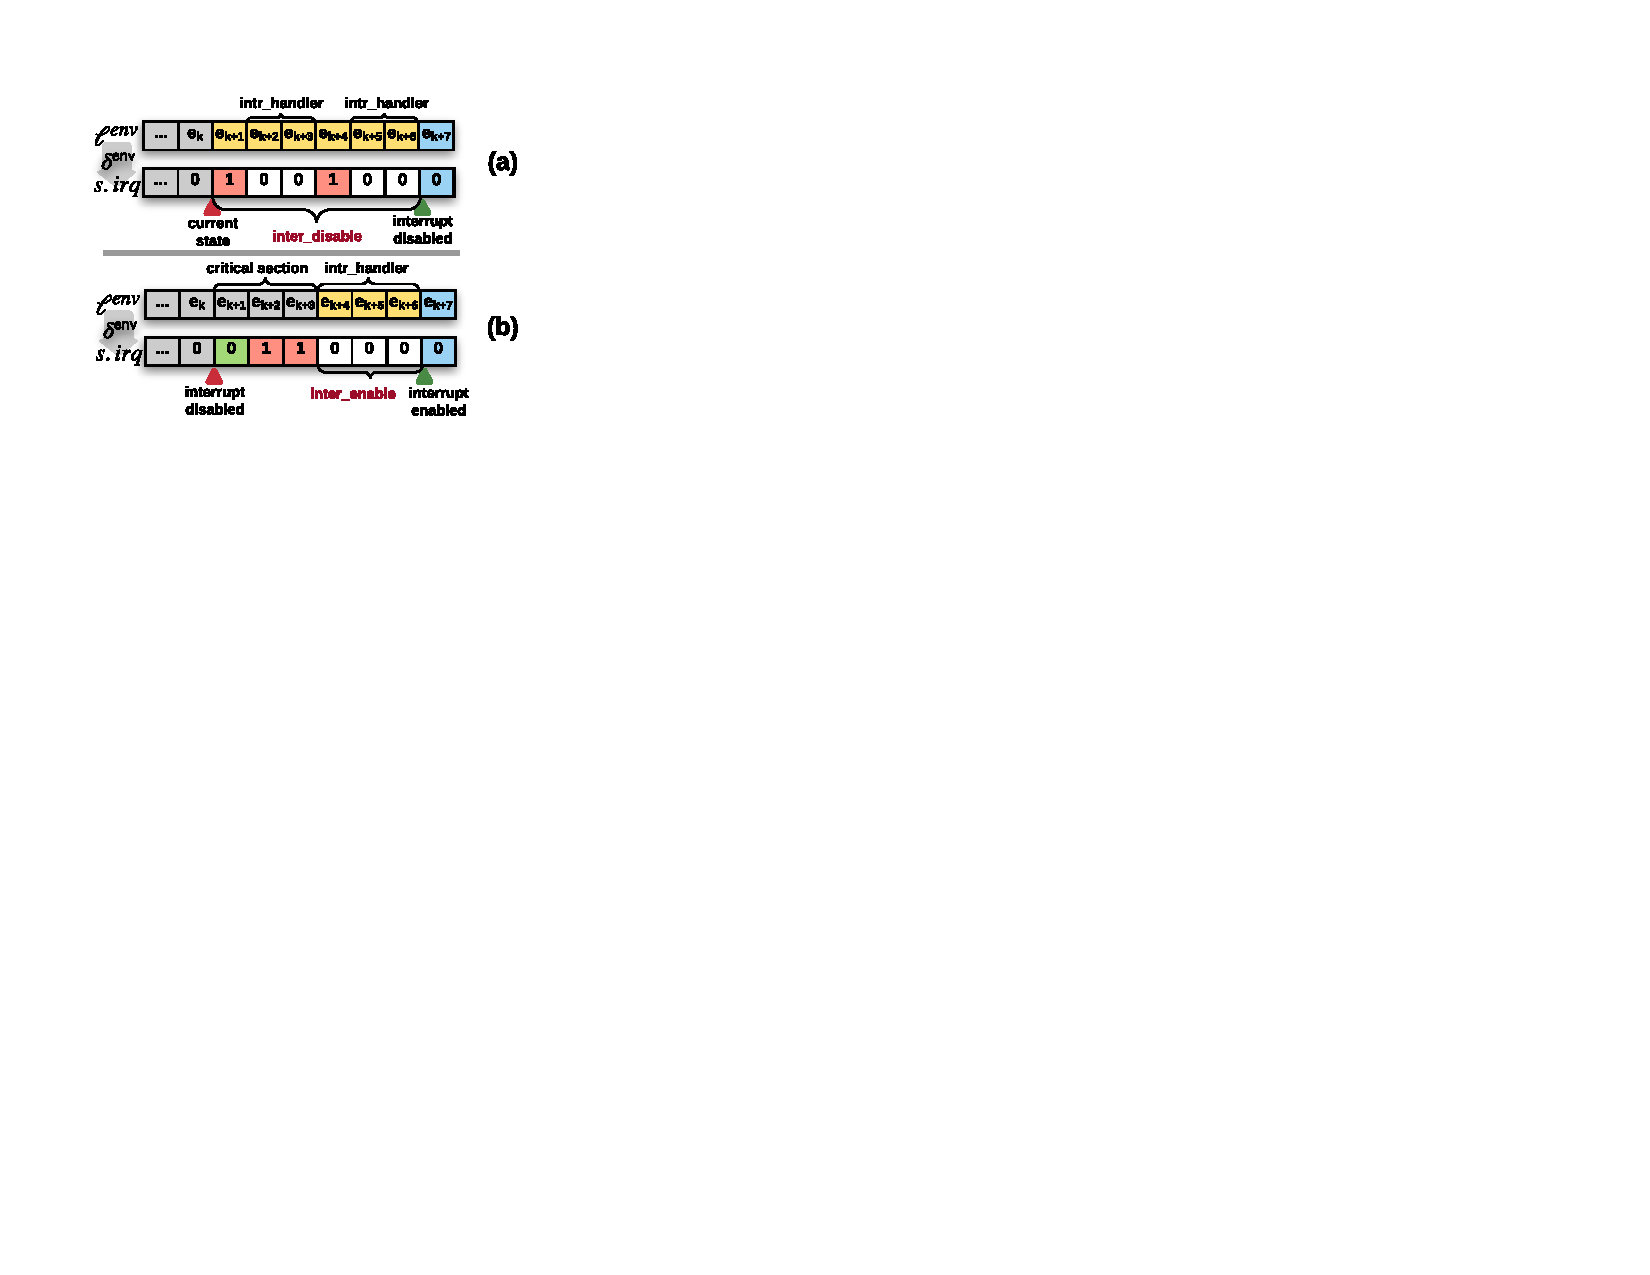
\includegraphics[scale=0.95]{figs/intr_enable}
\end{center}
\caption{Example behaviors of \texttt{intr\_disable} and \texttt{intr\_enable}.}
\label{fig:intr_enable}
\end{figure}
}




\ignore{
\paragraph{Contextual Refinement Between Two Interrupt Models} We uses several
steps to prove the contextual refinement between the two abstraction layers in
Fig.~\ref{fig:interrupt}. The goal of the refinement can be formalized as: for
device $D$ and a code fragment $f$ which ends with an primitive to disable /
enable interrupt of $D$, execution of that code on a hardware interrupt machine
is contextually equivalent to performing the same action on the abstract
interrupt machine. That is,
\[
\begin{array}{c}
\inferrule{
	(s_{hw}, m_{\mathsf{hw}}, \rho_{\mathsf{hw}}, s_{\textsf{IC\_hw}}, s_{D\_{\mathsf{hw}}}) \le_{R} (s_{abs}, m_{\mathsf{abs}}, \rho_{\mathsf{abs}}, s_{\textsf{IC\_abs}}, s_{D\_{\mathsf{abs}}}) \\
	(s'_{hw}, m'_{\mathsf{hw}}, \rho'_{\mathsf{hw}}, s'_{\textsf{IC\_hw}}, s'_{D\_{\mathsf{hw}}}, \ell'_i) =  \llbracket f \rrbracket_{\mathsf{hw}} (s_{hw}, m_{\mathsf{hw}}, \rho_{\mathsf{hw}}, s_{\textsf{IC\_hw}}, s_{D\_{\mathsf{hw}}}, \ell_i, \ell^{env}) \\
	(s'_{abs}, m'_{\mathsf{abs}}, \rho'_{\mathsf{abs}}, s'_{\textsf{IC\_abs}}, s'_{D\_{\mathsf{abs}}}, \ell'_i) =  \llbracket f \rrbracket_{\mathsf{abs}} (s_{abs}, m_{\mathsf{abs}}, \rho_{\mathsf{abs}}, s_{\textsf{IC\_abs}}, s_{D\_{\mathsf{abs}}}, \ell_i, \ell^{env}) \\
}{
	(s'_{hw}, m'_{\mathsf{hw}}, \rho'_{\mathsf{hw}}, s'_{\textsf{IC\_hw}}, s'_{D\_{\mathsf{hw}}}) \le_{R} (s'_{abs}, m'_{\mathsf{abs}}, \rho'_{\mathsf{abs}}, s'_{\textsf{IC\_abs}}, s'_{D\_{\mathsf{abs}}})
}
\end{array}
\]

Here, the evaluation of a code fragment takes an abstract state of kernel
$s$, the memory $m$, the register set $\rho$, the state of interrupt
controller $s_{\textsf{ic}}$, the state of the device $s_{D}$, a local log of
the device $\ell_i$, the event list $\ell^{env}$, and returns appropriate new
system states after the interrupt transition is fully performed.

Code fragment $f$ can be split into two disjoint parts: the part without the
last primitive ($f'$) and the last primitive ($p$). Let us assume that there is
no interrupt disabling and enabling for $D$ in the middle of $f'$. If there is, we can apply the same goal with that smaller fragment. The execution of $f$
in both machine is the sequential concatenation of the two parts:
\[
\inferrule {
	f = f'; p \\
	(s'_{os}, m', \rho', s'_{\textsf{IC}}, s'_{D}, \ell'_i) =  \llbracket f' \rrbracket (s_{os}, m, \rho, s_{\textsf{IC}}, s_{D}, \ell_i, \ell^{env}) \\
	(s''_{os}, m'', \rho'', s''_{\textsf{IC}}, s''_{D}, \ell''_i) =  \llbracket p \rrbracket (s'_{os}, m', \rho, s'_{\textsf{IC}}, s'_{D}, \ell'_i, \ell^{env})
} {
	(s''_{os}, m'', \rho'', s''_{\textsf{IC}}, s''_{D}, \ell''_i) =  \llbracket f \rrbracket (s_{os}, m, \rho, s_{\textsf{IC}}, s_{D}, \ell_i, \ell^{env})
}
\]

\noindent{}Case 1: $p$ is \texttt{intr\_disable}.

In the hardware interrupt machine, the execution of $\llbracket f'
\rrbracket_{\textsf{hw}}$ may interleave with interrupt transitions. To prove
the contextual refinement in this case, we first show that the result of these
transitions only change the state of the device, and then with the the isolation
policy, we show that all the interrupt transitions performed during the
execution of $f'$ equivalent to be done before \textsf{intr\_disable}.

\begin{figure}
	\begin{center}
	\[
	\begin{array}{c}
	\inferrule{
		(s'_{\textsf{ic}}, \textsf{IRQ} ~ n) = \texttt{intr}_{\textsf{IC}}(s_{\textsf{ic}}, N_D) \\\\
		(s',\rho') = \texttt{intr}_{\textsf{CPU}}(s, \rho, \textsf{IRQ} ~ n) \\\\
		s''_{\textsf{ic}} = \texttt{eoi}(s'_{\textsf{ic}}) \\
		(s'_{D}, \ell'_i) = \texttt{intr\_handler}_{\textsf{D}}(s_{D}, \ell_i, \ell^{env}) \\
		(d'', \rho'') =  \texttt{iret} (s', \rho') 
	}{
	   \texttt{intr}(s, m, \rho, s_{\textsf{ic}}, s_{D}, \ell_i, \ell^{env})
          	\defeq	(s'', m, \rho'', s''_{\textsf{ic}}, s'_{D}, \ell'_i) 
	} 
	\end{array}
	\]
	\end{center}
	\caption{Interrupt transition for the whole system, in the case when an
	interrupt is triggered by the device $D$ on interrupt line number $N_D$. 
		}
	\label{fig:int-whole-system}
\end{figure}

\begin{lemma}\label{lemma:irq}
	An IRQ is transparent to the CPU and the IC, i.e., the transitions triggered
	by the IRQ only change the states of the corresponding device that triggered the interrupt.
\end{lemma}
\noindent{}\begin{myproof}
	When the interrupt is disabled on the CPU or the particular interrupt line is
masked in the IC, the proof is obvious. When the interrupt is enabled, i.e.,
the corresponding interrupt line is routed, not masked, and the
\textsf{EFLAGS.if} register bit is set, the state transition of the whole
system is shown in Fig.~\ref{fig:int-whole-system}.   In this case, we need to show that:
\[\begin{array}{c}
		\inferrule{
			(s', m', \rho', s'_{\textsf{ic}}, s'_{D}, \ell'_{i}) 
			= \texttt{intr}(s, m, \rho, s_{\textsf{ic}}, s_{D}, \ell_{i}, \ell^{env}) 
		}{
			(s'_{D}, \ell'_{i}) = \texttt{intr\_handler}_{\textsf{D}}(s_{D}, \ell_{i}, \ell^{env}) \wedge \\
			 s' = s \wedge m' = m \wedge \rho' = \rho \wedge s'_{\textsf{ic}} = s_{\textsf{ic}} 
		} 
  \end{array}\]
\noindent{}This can be proven by composing the interrupt transition
rules of the CPU and the IC with Lemma \ref{lemma:context} and Lemma \ref{lemma:intr-handler}.
\end{myproof}

\begin{corollary} \label{corollary:irq}
IRQs do not affect the kernel, i.e., they do not change any of the
kernel's states\footnote{Remember, we consider device drivers a part
  of the device, not the kernel.}.
\ignore{
More formally, let the predicate $\texttt{kernel\_states} ~s$ represent a record containing
all the kernel states in the global system state $s$, then
\[\begin{array}{c}
		\inferrule{
			\texttt{intr\_handler}(s) = s' \\
		}{
			\texttt{kernel\_states} ~s = \texttt{kernel\_states} ~s' \\
		} \\
		\end{array}
		\]
}
\end{corollary}

\begin{lemma}
The execution of $\llbracket f' \rrbracket$ in both machine will have the same
result of kernel abstract state $s$, memory $m$, register set $\rho$ and the
state of interrupt controller $s_{\textsf{IC}}$. That is,
\[
\inferrule{
	(s_{hw}, m_{\mathsf{hw}}, \rho_{\mathsf{hw}}, s_{\textsf{IC\_hw}}, s_{D\_{\mathsf{hw}}}) \le_{R} (s_{abs}, m_{\mathsf{abs}}, \rho_{\mathsf{abs}}, s_{\textsf{IC\_abs}}, s_{D\_{\mathsf{abs}}}) \\
	(s''_{hw}, m''_{\mathsf{hw}}, \rho''_{\mathsf{hw}}, s''_{\textsf{IC\_hw}}, s''_{D\_{\mathsf{hw}}}, \ell''_i) =  \llbracket f' \rrbracket_{\mathsf{hw}} (s_{hw}, m_{\mathsf{hw}}, \rho_{\mathsf{hw}}, s_{\textsf{IC\_hw}}, s_{D\_{\mathsf{hw}}}, \ell_i, \ell^{env}) \\
	(s''_{abs}, m''_{\mathsf{abs}}, \rho''_{\mathsf{abs}}, s''_{\textsf{IC\_abs}}, s''_{D\_{\mathsf{abs}}}, \ell''_i) =  \llbracket f' \rrbracket_{\mathsf{abs}} (s_{abs}, m_{\mathsf{abs}}, \rho_{\mathsf{abs}}, s_{\textsf{IC\_abs}}, s_{D\_{\mathsf{abs}}}, \ell_i, \ell^{env}) \\
}{
	s''_{hw} \le_{R} s''_{abs} \\
	m''_{hw} \le_{R} m''_{abs} \\
	\rho''_{hw} \le_{R} \rho''_{abs} \\
	s''_{\textsf{IC\_hw}} \le_{R} s''_{\textsf{IC\_hw}} \\
}
\]
\end{lemma}

\noindent{}\begin{myproof}
From the Corollary~\ref{corollary:irq}, the interrupt transitions only change
the state of devices. Thus, even there is interleaving in the execution of
$\llbracket f' \rrbracket_{hw}$, it will not affect the transition of kernel and
IC.
\end{myproof}

\begin{lemma}
	After executes the same number of $\texttt{intr\_handler}_D$ in the abstract
interrupt machine at the end of $\llbracket f' \rrbracket_{abs}$, the device
state will be the same as the hardware interrupt one. The number depends on $\ell^{env}$.
	\[
	\inferrule{
		(s_{hw}, m_{\mathsf{hw}}, \rho_{\mathsf{hw}}, s_{\textsf{IC\_hw}}, s_{D\_{\mathsf{hw}}}) \le_{R} (s_{abs}, m_{\mathsf{abs}}, \rho_{\mathsf{abs}}, s_{\textsf{IC\_abs}}, s_{D\_{\mathsf{abs}}}) \\
		(s''_{hw}, m''_{\mathsf{hw}}, \rho''_{\mathsf{hw}}, s''_{\textsf{IC\_hw}}, s''_{D\_{\mathsf{hw}}}, \ell''_i) =  \llbracket f' \rrbracket_{\mathsf{hw}} (s_{hw}, m_{\mathsf{hw}}, \rho_{\mathsf{hw}}, s_{\textsf{IC\_hw}}, s_{D\_{\mathsf{hw}}}, \ell_i, \ell^{env}) \\
		(s''_{abs}, m''_{\mathsf{abs}}, \rho''_{\mathsf{abs}}, s''_{\textsf{IC\_abs}}, s''_{D\_{\mathsf{abs}}}, \ell_i) =  \llbracket f' \rrbracket_{\mathsf{abs}} (s_{abs}, m_{\mathsf{abs}}, \rho_{\mathsf{abs}}, s_{\textsf{IC\_abs}}, s_{D\_{\mathsf{abs}}}, \ell_i, \ell^{env}) \\
		(s'''_{D\_{\mathsf{abs}}}, \ell'''_i) = \texttt{intr\_handler\_next} (s''_{D\_{\mathsf{abs}}}, \ell''_i, \ell^{env}) 
		}{
		s'''_{D\_{\mathsf{abs}}} \le_{R} s''_{D\_{\mathsf{hw}}}
	}
	\],
\noindent{}where \texttt{intr\_handler\_next} is defined as:
\[
\inferrule{
	(e,\ell'_i) = \textsf{next} (\ell^{env}, \ell_i) \\	
	s' = \delta^{\textsf{env}} (s, e) \\
	s'.irq = \textsf{true} \\
	(s'', \ell_i'') = \texttt{intr\_handler} (s', \ell'_i, \ell^{env}) \\
	(s''', \ell_i''') = \texttt{intr\_handler\_next} (s'', \ell''_i, \ell^{env}) \\
}{
	\texttt{intr\_handler\_next} (s, \ell_i, \ell^{env}) \defeq (s''', \ell_i''') 
}
\]
\[
\inferrule{
	(e,\ell'_i) = \textsf{next} (\ell^{env}, \ell_i) \\	
	s' = \delta^{\textsf{env}} (s, e) \\
	s'.irq = \textsf{false} \\
}{
	\texttt{intr\_handler\_next} (s, \ell_i, \ell^{env}) \defeq (s, \ell_i) 
}
\]
\end{lemma}

\noindent{}\begin{myproof}
From the Lemma~\ref{lemma:intr-handler}, the interrupt transitions do not depend
on the state of kernel and other devices, so the result of the interrupt handler
is location independent.
\end{myproof}

\begin{lemma}
	The execution of the interrupt disabling in both machine keeps the refinement
relation.
\end{lemma}
\noindent{}\begin{myproof}
In the hardware interrupt model, we use $\texttt{mask}~n$ to disable the
interrupt for a certain device. This $n$ is unique and the mask bit of $n$ is
mapped to the $\textsf{critical}$ flag in the abstract level. When the interrupt
line is masked, $\textsf{critical} = \textsf{true}$, and otherwise
$\textsf{critical} = \textsf{false}$. This relation is proved by its definition.
\end{myproof}

\noindent{}Case 2: $p$ is \texttt{intr\_enable}.

This means the interrupt is disabled in the $f'$. It is true that we can also
call \texttt{intr\_enable} when the interrupt is enabled. However, the semantics
of this equivalent to \textsf{nop}. Thus, we forbid calling interrupt disable /
enable function that is not paired.

\begin{lemma}
	The execution of $\llbracket f' \rrbracket$ is the same for both machine when the interrupt is disabled.
\end{lemma}
\noindent{}\begin{myproof}
If the interrupt is disabled, there is no interleaving of $f'$ and interrupt
handler. The device will set its \textsf{irq} state to \textsf{true} if
$\delta^{env}$ generate an interrupt request. However, as proved in
Lemma~\ref{lemma:irq}, the transition of IC does not change the state of IC if
the interrupt is routed incorrectly, masked or $\textsf{EFLAGS.if} = 0$.
\end{myproof}

The only difference is the last primitive. If there are pending IRQs during the
interrupt disabled execution, when the interrupt is enabled, the interrupt
handler will be executed immediately. It is the same for both machine.
}

\paragraph{Contextual Refinement Between Two Interrupt Models}
To show the contextual refinement between the two abstraction layers
in Fig.~\ref{fig:interrupt}, we prove that the behavior of an IRQ
can indeed be made transparent to the CPU and the IC.


\begin{figure}
	\begin{center}
\begin{small}
	\[
	\begin{array}{cr}
	\inferrule{
		(s'_{\textsf{ic}}, \textsf{IRQ} ~ n) = \texttt{intr}_{\textsf{IC}}(s_{\textsf{ic}}, N_D) \\
		(d',\rho') = \texttt{intr}_{\textsf{CPU}}(d, \rho, \textsf{IRQ} ~ n) \\
		s''_{\textsf{ic}} = \texttt{eoi}(s'_{\textsf{ic}}) \\
		(s'_{D}, \ell'_i) = \texttt{intr\_handler}_{\textsf{D}}(s_{D}, \ell_i, \ell^{env}) \\
		(d'', \rho'') =  \texttt{iret} (d', \rho') 
	}{
	   \texttt{intr}(d, m, \rho, s_{\textsf{ic}}, s_{D}, \ell_i, \ell^{env})
          	\defeq	(d'', m, \rho'', s''_{\textsf{ic}}, s'_{D}, \ell'_i) 
	} & (\texttt{normal}) \\ [5ex]
	\inferrule{
		(s'_{\textsf{ic}}, \emptyset) = \texttt{intr}_{\textsf{IC}}(s_{\textsf{ic}}, N_D)
	}{
		\texttt{intr}(d, m, \rho, s_{\textsf{ic}}, s_{D}, \ell_i, \ell^{env})
		\defeq	(d, m, \rho, s'_{\textsf{ic}}, s_{D}, \ell_i) 
	} & (\texttt{{masked}}) \\ [5ex]
	\inferrule{
		(s'_{\textsf{ic}}, \textsf{IRQ} ~ n) = \texttt{intr}_{\textsf{IC}}(s_{\textsf{ic}}, N_D) \\
		\textsf{IDT}[n] = \textsf{None}
	}{
		\texttt{intr}(d, m, \rho, s_{\textsf{ic}}, s_{D}, \ell_i, \ell^{env})
		\defeq	\textsf{None} 
	} & (\texttt{not routed}) \\ [5ex]
	\inferrule{
		(s'_{\textsf{ic}}, \textsf{IRQ} ~ n) = \texttt{intr}_{\textsf{IC}}(s_{\textsf{ic}}, N_D) \\
		\rho[\textsf{EFLAGS}.\textsf{if}] = \textsf{Disabled} \\\\
		(d',\rho') = \texttt{intr}_{\textsf{CPU}}(d, \rho, \textsf{IRQ} ~ n) \\
	}{
		\texttt{intr}(d, m, \rho, s_{\textsf{ic}}, s_{D}, \ell_i, \ell^{env})
		\defeq	(d', m, \rho', s_{\textsf{ic}}, s_{D}, \ell_i) 
	} & (\texttt{disabled})
	\end{array}
	\]
\end{small}
	\end{center}
	\caption{Interrupt transition for the whole system, in the case when an
	interrupt is triggered by the device $D$ on interrupt line number $N_D$. 
		}
	\label{fig:int-whole-system}
\end{figure}

\begin{lemma}
	An IRQ is transparent to the CPU and the IC, i.e., the transitions triggered
	by the IRQ only change the states of the corresponding device that triggered the interrupt.
\end{lemma}
\noindent{}\begin{myproof}
When the interrupt is disabled on the CPU or the particular
interrupt line is masked in the IC, the proof is obvious.
When the interrupt is enabled, i.e., the corresponding
interrupt line is routed, not masked, and the
\textsf{EFLAGS.if} register bit is set, the state transition
of the whole system is shown in Fig.~\ref{fig:int-whole-system}.
Here, the transition
$\texttt{intr}$ takes an abstract state $d$, the memory $m$,
the register set $\rho$, the state of interrupt controller
$s_{\textsf{ic}}$, the state of the device $s_{D}$, a local
log of the device $\ell_i$, the event list $\ell^{env}$, and
returns appropriate new system states after the interrupt
transition is fully performed.  In this case, we need to show
that:

\[\begin{array}{c}
		\inferrule{
			(d', m', \rho', s'_{\textsf{ic}}, s'_{D}, \ell'_{i}) 
			= \texttt{intr}(d, m, \rho, s_{\textsf{ic}}, s_{D}, \ell_{i}, \ell^{env}) 
		}{
			(s'_{D}, \ell'_{i}) = \texttt{intr\_handler}_{\textsf{D}}(s_{D}, \ell_{i}, \ell^{env}) \wedge 
			 d' = d \wedge m' = m \wedge \rho' = \rho \wedge s'_{\textsf{ic}} = s_{\textsf{ic}} 
		} 
  \end{array}\]

\noindent{}This can be proven by composing the interrupt transition
rules of the CPU and the IC with Lemma \ref{lemma:context}.
\footnote{In our IC model, the middle states in the transition of interrupt delivery are
discarded if the interrupt is not successfully handled. In the case when the
interrupt is disabled in the CPU but not masked in the IC, the states of IC
fallback to their original value. This model is still valid in the sense that
we can delay this state change of IC until the next time when the interrupt
is raised again for that particular device and gets handled successfully.
}
\end{myproof}

\begin{corollary}
IRQs do not affect the kernel, i.e., they do not change any of the
kernel's states\footnote{Remember, we consider device drivers a part
  of the device, not the kernel.}.
\ignore{
More formally, let the predicate $\texttt{kernel\_states} ~s$ represent a record containing
all the kernel states in the global system state $s$, then
\begin{small}\[\begin{array}{c}
		\inferrule{
			\texttt{intr\_handler}(s) = s' \\
		}{
			\texttt{kernel\_states} ~s = \texttt{kernel\_states} ~s' \\
		} \\
		\end{array}
		\]
\end{small}
}
\end{corollary}



\begin{figure}
	\begin{center}
	\[
	\begin{array}{c}
	\inferrule{
		(s'_{\textsf{ic}}, \textsf{IRQ} ~ n) = \texttt{intr}_{\textsf{IC}}(s_{\textsf{ic}}, N_D) \\\\
		(d', \rho') = \texttt{intr}_{\textsf{CPU}}(d, \rho, \textsf{IRQ} ~ n) \\\\
		s''_{\textsf{ic}} = \texttt{eoi}(s'_{\textsf{ic}}) \\
		s'''_{\textsf{ic}} = \texttt{mask}(s''_{\textsf{ic}}, N_D) \\
		(d'', \rho'') = \texttt{sti}(d', \rho') \\
		(s'_{D}, \ell'_i) = \texttt{intr\_handler}_{\textsf{D}}(s_{D}, \ell_i, \ell^{env}) \\
		(d''', \rho''') = \texttt{cli}(d'', \rho'') \\
		s''''_{\textsf{ic}} = \texttt{unmask}(s'''_{\textsf{ic}}, N_D) \\
		(d'''', \rho'''') =  \texttt{iret} (d''', \rho''') 
	}{
	 \texttt{intr}(d, m, \rho, s_{\textsf{ic}}, s_{D}, \ell_i, \ell^{env})
      	\defeq	(d'''', m, \rho'''', s''''_{\textsf{ic}}, s'_{D}, \ell'_i) 
	}\end{array}\]
	\end{center}
	\caption{Interrupt transition for the whole system when
          nested interrupts are allowed.}
	\label{fig:int-whole-system-nested}
\end{figure}


\begin{figure}
	\begin{center}
		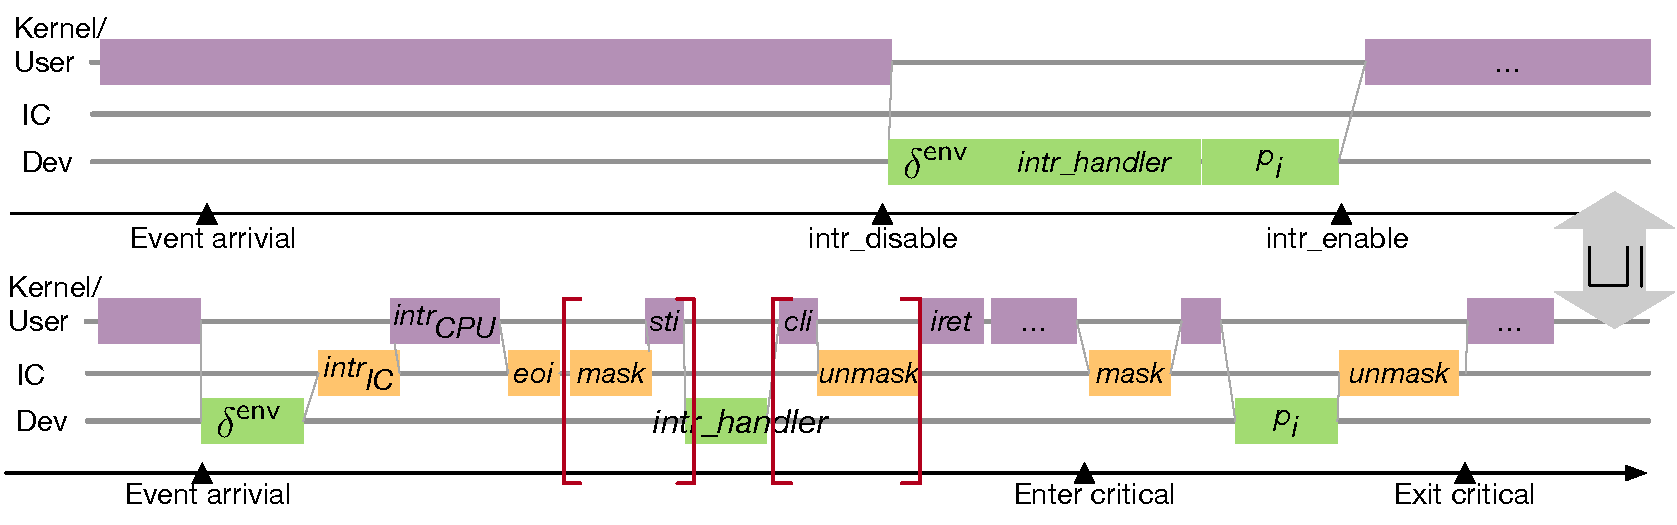
\includegraphics[width=0.95\textwidth]{figs/interrupt_nest}
	\end{center}
	\caption{The contextual refinement between interrupt models with nested interrupts.}
	\label{fig:intr_enable_nested}
\end{figure}


At this abstract interrupt model, every access to the device's abstract
states needs to be guarded by a call to {\it intr\_disable}, and this
is systematically enforced through explicit preconditions of all device primitives. 
Note that at this level, an interrupt handler of a device only changes
abstract states of that particular device. Thus, the correctness of
deferring handling all the interrupts to {\it intr\_disable} and {\it intr\_enable}
naturally follows, as none of the ``non-critical'' steps outside the pair
can change the states of the device, nor reading any states of the device.


\subsubsection{Nested Interrupts}

Note that the $\texttt{intr}_{\textsf{CPU}}$ transition in
Fig.~\ref{fig:interrupt-cpu} disables the interrupt. Thus between
$\texttt{intr}_{\textsf{CPU}}$ and $\texttt{iret}$ in
Fig.~\ref{fig:int-whole-system}, the interrupt is turned off, which means that
no nested interrupts are allowed. In many cases, supporting nested interrupts is
critical so that some high priority interrupt processing is not delayed by the
low priority ones.  The interrupt transition for the whole system with nested
interrupts is shown in Fig.~\ref{fig:int-whole-system-nested}.  Here, before the
interrupt handler is called, we mask the interrupt line of the particular device
(to make sure there is no nested interrupt from the same device) and then turn
on the interrupt on the CPU. Accordingly, after the interrupt handling, we
disable the CPU interrupt, then unmask the particular interrupt line before the
$\texttt{iret}$ transition is performed.  We have proved that this model also
refines the same abstract interrupt model (see
Fig.~\ref{fig:intr_enable_nested}).

\ignore{
\begin{lemma}
	IRQs do not affect the kernel\footnote{Remember, we consider device drivers 
	a part of the device, not the kernel.}.
\end{lemma}
\begin{myproof}
	The proof can be done through case analysis. 
	\begin{itemize}	
	\item If the particular interrupt line is masked in the IC, the CPU does not
	receive the interrupt request.

	\item If the interrupt line is not masked, but interrupts are disabled on 
	the	CPU, the interrupt signal is ignored.

	\item If the interrupt line is not masked and interrupts are enabled, the 
	CPU receives the interrupt signal and performs its own {\it intr} 
	transition. The state transition of the whole system is shown in
        Fig.~\ref{fig:int-whole-system}.
        Thus, it is sufficient to show that $d'' = d$, 
	$m'' = m$, and $\rho'' = \rho$. These can be proven by composing the 
	{\it intr} and {\it iret} with Lemma \ref{lemma:context}.
		

\end{itemize}

\end{myproof}


\begin{lemma}
An IRQ is transparent to the IC. 
\end{lemma}
\begin{myproof}
If the particular interrupt line is masked, the IC ignores the interrupt.
Otherwise, the IC does its {\it intr} transition, and the signal goes to
the CPU. If interrupts are enabled in that CPU, then CPU performs the relevant
transition, otherwise, if the interrupt is disabled, the interrupt eventually 
gets handled by the CPU when the CPU enables the interrupt through {\it sti}. 
In either case, the {\it eoi} primitive in IC is called (see
Fig.~\ref{fig:int-whole-system}).\footnote{If the CPU never re-enables another 
interrupt, its correctness is independent of what interrupt gets triggered.}
\end{myproof}
}

%\asectskip

	 % Device driver verification
%\section{A More Realistic Device and Interrupt Model}
%\input{model}	 % More realistic machine model
\section{Case Study}
\label{sec:case_study}

\begin{figure}
	\begin{center}
		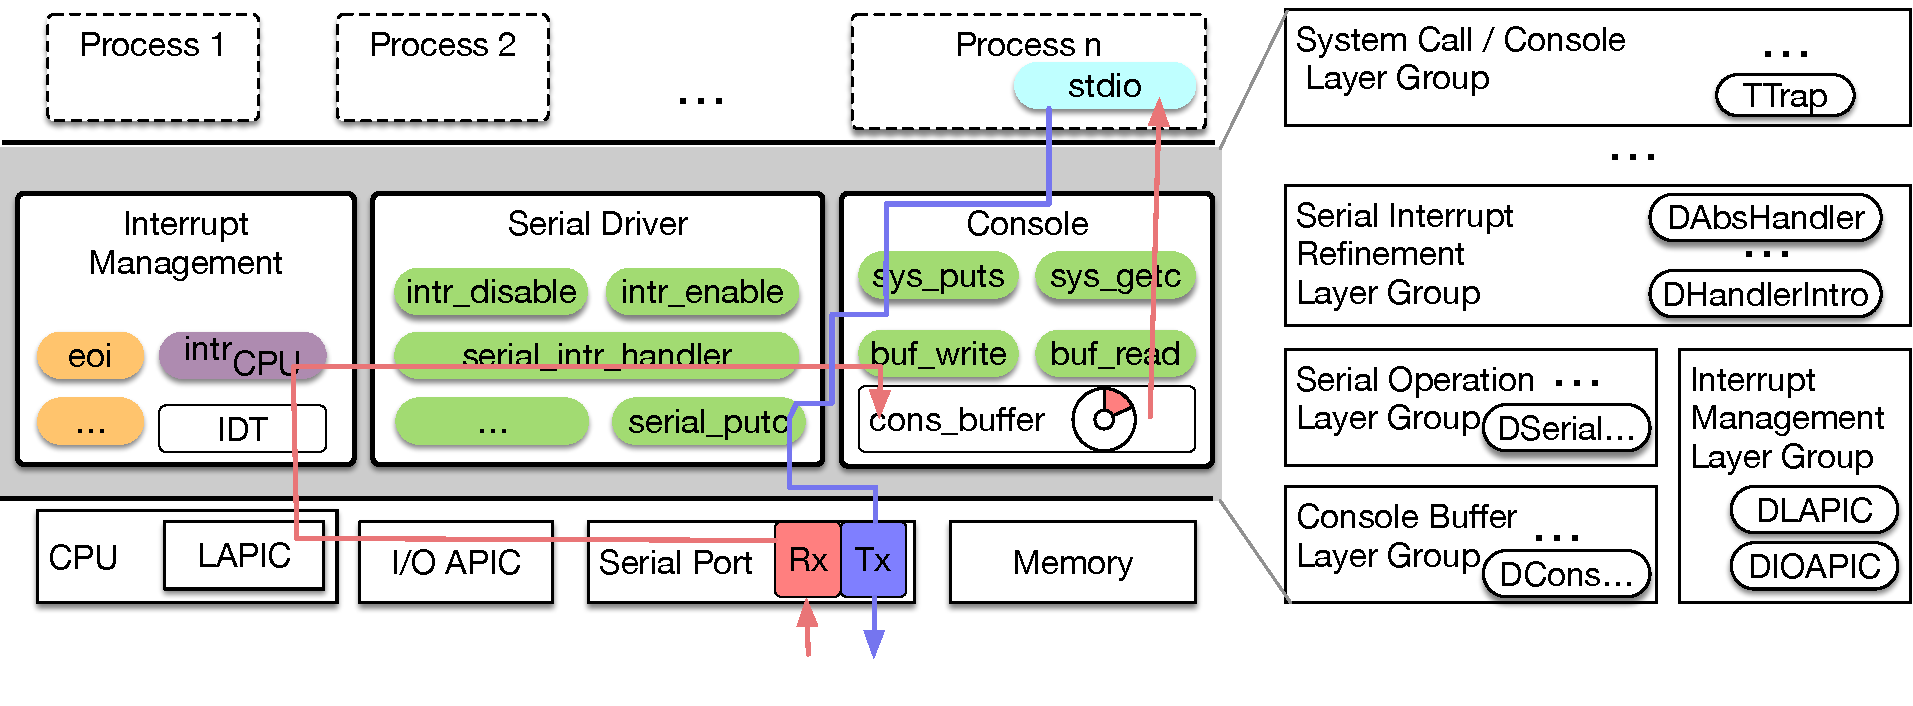
\includegraphics[scale=0.35]{figs/data_flow}
	\end{center}
	\caption{The data-flow of serial console messages and corresponding layer decomposition}
	\label{fig:data-flow}
\end{figure}


In this section, we present case studies of our verified drivers.
Fig.~\ref{fig:data-flow} shows the overall structure of our verified serial
console, while the left side reflects how the implementation of driver modules
organized as well as the data/control flow. The right side gives an overview
of how those modules are verified through the construction of certified layers. We have
used a single controller in Sec.~\ref{sec:driver} to make the presentation
concise. However, mCertiKOS utilizes two physical interrupt controller devices:
the I/O Advanced Programmable Interrupt Controller (I/O APIC) and the Local
Advanced Programmable Interrupt Controller (Local APIC). Together with the
serial device, we present the formal models of these three hardware devices
throughout this section.

As shown in Fig.~\ref{fig:data-flow}, at the system call level, users can invoke
relevant system calls (\text{sys\_getc}, \text{sys\_puts}, {\it etc}) to read
from or write to the serial port. The red lines in the figure represent the
flow of receiving data from the serial port. The implementation is interrupt driven.
Thus, when the serial receiving buffer (Rx) gets new data, the device triggers
an interrupt that goes through the Local APIC and I/O APIC devices and the
interrupt handler of the serial device stores the data into the console circular
buffer (\texttt{cons\_buffer}). Later, when a user process makes the system call
\text{sys\_getc}, the system call handler simply pops and returns the head of
\texttt{cons\_buffer}. On the transmitting side, writing data to the serial port
(blue lines in the figure) is completely synchronous. When the system call
\texttt{sys\_puts} is invoked, the system call handler calls the transmission
function \texttt{serial\_putc} of the serial driver to write data to the
transmission buffer (Tx) of the serial device. The critical sections are protected
by the functions \texttt{serial\_intr\_disable} and
\texttt{serial\_intr\_disable} which masks and unmasks the interrupt signal of
the serial device.

The verification of the console circular buffer (\texttt{cons\_buffer}) is
already presented in Chapter \ref{chapter:framework}. In this section, we also present
the formal model and verification of their drivers for the serial port, I/O
APIC, and Local APIC.

\subsection{Serial Port}

Fig.~\ref{fig:serial} illustrates a typical serial port with a bounded internal
buffer of size 12. It consists of an RS-232 interface and a Universal
Asynchronous Receiver/Transmitter (UART) controller. RS-232 delivers electrical
signals between the UART controller and the connection cable. The UART controller
is responsible for demodulating received data into digital bits and storing them
into the internal receiving (Rx) buffer, and also modulating sent data from
digital bits and inserting them into the transmission (Tx) buffer.

The hardware UART controller has many features, and the mCertiKOS serial driver
only utilizes those parts needed for sending and receiving character strings.
When modeling the serial port, we take the minimalistic approach of only
modeling the set of features utilized by the existing drivers. The internal
state of the serial port device is defined as:

\begin{definition} \label{def:serial-device}
	Abstract state of serial device.
\[
\begin{array}{lll}
s = ( & \mathsf{RxBuf}: \mathsf{list} ~ \mathsf{char}, & \vartriangleright \textit{Receiving buffer} \\
 & \mathsf{TxBuf}: \mathsf{list} ~ \mathsf{char}, & \vartriangleright \textit{Transmission buffer} \\
 & \mathsf{irq}: \mathsf{bool}, & \vartriangleright \textit{Interrupt pending} \\
 & \mathsf{Connected}: \mathsf{bool}, & \vartriangleright \textit{Power} \\
 & \mathsf{Base}: \mathbb{Z}, & \vartriangleright \textit{Base address} \\
 & \multicolumn{2}{l} {\vartriangleright \textit{Line and modem configurations:}} \\
 & \multicolumn{2}{l}{\mathsf{RxIntEnable}: \mathsf{bool}, ~ \mathsf{DLAB}: \mathsf{bool}, ~ \mathsf{Baudrate}: \mathbb{Z},} \\
 & \multicolumn{2}{l}{\mathsf{Databits}: \mathbb{Z}, ~ \mathsf{Stopbits}: \mathbb{Z}, ~ \mathsf{Parity}: \mathsf{ParityType},} \\
 & \mathsf{FIFO}: \mathbb{Z}, ~ \mathsf{Modem}: \mathbb{Z} ~). \\
\end{array}
\]
\end{definition}
		
There are three external events for the serial device. The serial event
$\textsf{Recv}~ s$ indicates that a string has been received. The
$\textsf{SendingCompAck}$ event implies the device received the acknowledgment
that the characters in the transmission buffer have been sent out successfully,
while the $\textsf{NoSendingCompAck}$ event indicates that the sending of
characters in the transmission buffer is not yet complete.

The serial device is configured to trigger an interrupt when it receives data (a
non-empty string), and not to trigger an interrupt when the transmission buffer
becomes empty, i.e., when the characters in the transmission buffer are sent out
successfully. Thus, before any data is written to the serial port, we have to
poll the transmission status until it becomes empty. We have chosen this setup
because it covers both interrupt-triggering and polling events.

Note that, the states $s.\mathsf{RxBuf}$ and $s.\mathsf{irq}$ are disjoint from
$s.\mathsf{TxBuf}$ under the environment transitions in that the former is for
receiving data and the latter is for sending data only.  This allows us to use
two separate local logs in our device model, $\ell_{\textsf{tx}}$ (for
transmission) and $\ell_{\textsf{rx}}$ (for receiving), to handle these possibly
commutative events.

\begin{figure}
	\begin{center}
		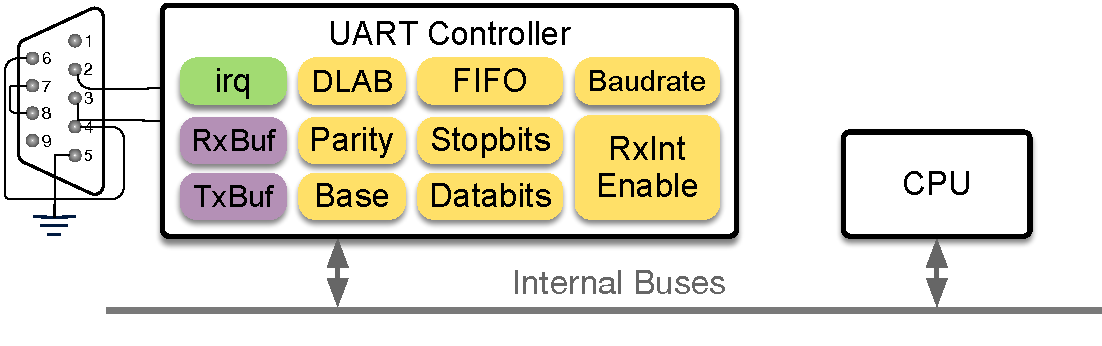
\includegraphics[scale=0.4]{figs/serial}
	\end{center}
	\caption{The hardware connections of a serial port}
	\label{fig:serial}
\end{figure}

\begin{figure}
\[
\begin{array}{cr}
	\inferrule{
		s.\mathsf{Connected} = \textsf{true} \\
		s.\mathsf{RxIntEnable} = \textsf{true} \\
		e = \mathsf{Recv} ~ w \\\\
		w \neq nil \\
		\textsf{newBuf} = \texttt{last}(\mathsf{BufSize}, (s.\mathsf{RxBuf} \textsf{++} w))
	}{
	  \delta^{\textsf{env}} (s, e) \defeq s[\mathsf{RxBuf} \leftarrow \textsf{newBuf}][\mathsf{irq} \leftarrow \textsf{true}]
	} & \text{(recvd\_irq)} \\[5ex]

	\inferrule{
	s.\mathsf{Connected} = \textsf{true} \\
	s.\mathsf{RxIntEnable} = \textsf{false} \\
	e = \mathsf{Recv} ~ w \\\\
	w \neq nil \\
	\textsf{newBuf} = \texttt{last}(\mathsf{BufSize}, (s.\mathsf{RxBuf} \textsf{++} w))
}{
	\delta^{\textsf{env}} (s, e) \defeq s[\mathsf{RxBuf} \leftarrow \textsf{newBuf}]
} & \text{(recvd\_no\_irq)} \\[5ex]

	\inferrule{
		s.\mathsf{Connected} = \textsf{true} \\
		e = \mathsf{Recv} ~ w \\
		w = nil 
	}{
		\delta^{\textsf{env}} (s, e) \defeq s
	} & \text{(norcv)} \\[5ex]

	\inferrule{
		s.\mathsf{Connected} = \textsf{true} ~~~~
		e = \mathsf{SendingCompAck} 
	}{
		\delta^{\textsf{env}} (s, e) \defeq s[\mathsf{TxBuf} \leftarrow \emptyset]
} & \text{(sent)} \\[5ex]

	\inferrule{
		s.\mathsf{Connected} = \textsf{true} ~~~~
		e = \mathsf{NoSendingCompAck} 
	}{
		\delta^{\textsf{env}} (s, e) \defeq s
} & \text{(noack)} \\[5ex]

	\inferrule{
		s.\mathsf{Connected} = \textsf{true} \\
		o = \textsf{input} ~ n \\\\
		n = s.\mathsf{Base} + 0 ~~~~
		s.\mathsf{DLAB} = \textsf{false} ~~~~
		s.\mathsf{RxBuf} = w \\
	}{
		\delta^{\textsf{CPU}} (s, o) \defeq s[\mathsf{RxBuf} \leftarrow \texttt{tl} ~ w ][\mathsf{irq} \leftarrow \textsf{false}] 
        } & \text{(read)} \\[5ex]
        
\inferrule{
	s.\mathsf{Connected} = \textsf{true} \\
	o = \textsf{output} ~ n ~ v\\\\
	n = s.\mathsf{Base} + 0 ~~~~
	s.\mathsf{DLAB} = \textsf{false} ~~~~
	s.\mathsf{TxBuf} = w \\
	}{\delta^{\textsf{CPU}} (s, o) \defeq s[\mathsf{TxBuf} \leftarrow \texttt{last}(\mathsf{BufSize}, (w \textsf{++} [v]))]\hspace*{-0.05in}
	} & \text{(write)} \\[5ex]

\inferrule{
	s.\mathsf{Connected} = \textsf{true} \\
	o = \textsf{output} ~ n ~ v\\\\
	n = s.\mathsf{Base} + 0 ~~~~
	s.\mathsf{DLAB} = \textsf{true} ~~~~
	r = (s.\mathsf{Baudrate}~\&~\mathsf{0xff00})~|~v \\
}{\delta^{\textsf{CPU}} (s, o) \defeq s[\mathsf{Baudrate} \leftarrow r]} & \text{(baudrate\_low)}
\end{array}
\]
\caption{The environment and CPU transition functions}
\label{fig:env-cpu-trans}
\end{figure}

Next, in Fig.~\ref{fig:env-cpu-trans}, we define the transition functions
$\delta^{\textsf{env}}$ and $\delta^{\textsf{CPU}}$, where
$\delta^{\textsf{env}}$ needs to handle all the possible environmental events
against the current state, and $\delta^{\textsf{CPU}}$ updates the current state
based on the input and output addresses and values. Note that function
\texttt{last} is used to model the action of dropping some elements in the front
of the buffer when the length of the new buffer exceeds the hardware buffer size
($\mathsf{BufSize}$). The \textsf{baud\_low} in Fig.~\ref{fig:env-cpu-trans} is an
example configuration of the control registers. The value of
\textsf{Baudrate} is not used to simulate the timing of the signal but
is checked against the real hardware settings in certain transitions, such
as $\delta^{\textsf{CPU}}$ for \textsf{read} and \textsf{write}, in order to
verify that the driver is free of misconfiguration bugs.

% The following rules exhibit some interesting transitions.

By instantiating the device state and transition functions from our general
device model in Sec.~\ref{sec:model}, we create a concrete model of the serial
port with the \texttt{read} and \texttt{write} primitives.

\begin{figure}
	\lstinputlisting [language=C, multicols=2] {src/serial_putc.c}
	\caption{The implementation of \texttt{serial\_putc} and \texttt{serial\_getc} in C}
	\label{fig:serial_putc}
	\vspace{-10pt}
\end{figure}

Next, we show how the drivers are specified and verified on top of this model.
Fig.~\ref{fig:serial_putc} shows code fragments of the function
\texttt{serial\_putc} and \texttt{serial\_getc}.  There, the
\texttt{serial\_read} and \texttt{serial\_write} are the two primitives in the
serial hardware model, while \texttt{get\_serial\_exist} is a new primitive (already
verified in some underlay) indicating whether the serial device is already
initialized. The if statement (line 3) prevents any misuse of
\texttt{serial\_putc()} before initialization.

For \texttt{serial\_putc}, if the $s.\textsf{TxBuf}$ buffer is initially empty,
or the device receives a $\textsf{SendingCompAck}$ event during the loop (line
4-6), the program sends the character \texttt{c} to the serial port (line 8).
The function \texttt{serial\_putc} is specified as follows:
\[
	\inferrule{
		s.\mathsf{TxBuf} = \emptyset \\
		s.\mathsf{get\_serial\_exist} = \textsf{true} \\\\
		s' = s[\mathsf{TxBuf} \leftarrow [c]] \\
		(e, \ell'_{\textsf{tx}}) = \texttt{next}(\ell^{env}, \ell_{\textsf{tx}}) \\
		(e', \ell''_{\textsf{tx}}) = \texttt{next}(\ell^{env}, \ell'_{\textsf{tx}})
	}{
	\texttt{serial\_putc} (s, c, \ell_{\textsf{tx}}, \ell^{env}) \defeq (s', \ell''_{\textsf{tx}})
	}
\]
\[
\inferrule{
	s.\mathsf{TxBuf} \neq \emptyset \\
	s.\mathsf{get\_serial\_exist} = \textsf{true} \\
	(e, \ell'_{\textsf{tx}}) = \texttt{next}(\ell^{env}, \ell_{\textsf{tx}}) \\
	s' = \delta^{env}(s, e) \\
	(s'', \ell''_{\textsf{tx}}) = \texttt{serial\_putc} (s', c, \ell'_{\textsf{tx}}, \ell^{env}) \\
}{
\texttt{serial\_putc} (s, c, \ell_{\textsf{tx}}, \ell^{env}) \defeq (s'', \ell''_{\textsf{tx}})
}
\]

The first rule above shows the case when the transmission buffer is
originally empty. Here, $\textsf{lsr}$ immediately becomes $1$ in the
first loop iteration, and the character is written to the transmission
buffer in the device right away. Note that the function \textsf{next}
is called twice because the implementation of \textsf{serial\_putc} has
two serial I/O operations for the base case: one to check whether the
transmission buffer is empty, and the other to put the
character into the transmission buffer. 

The second rule above shows the case when the initial transmission buffer
is not empty. Here, the device performs transition based on
the received event $e$ and repeats the same process until it finally
receives the $\textsf{SendingCompAck}$ event. Then, by definition of
$\delta^{env}$ in Fig.~\ref{fig:env-cpu-trans}, the transmission
buffer becomes empty and the next recursive call falls into the first
case of the specification.

As for \texttt{serial\_getc}, a check of the status register will be first performed
to clear the \textsf{IRQ} state and confirm that there are pending receiving
messages (line 16). If the receiving buffer is not empty, the head of the buffer is
fetched (line 17) and inserted into the console buffer.

\begin{figure}
	\lstinputlisting [language=C] {src/serial_puts.c}
	\caption{The implementation of \texttt{serial\_puts} in C}
	\label{fig:serial_puts}
	\vspace{-10pt}
\end{figure}

In Fig.~\ref{fig:serial_puts}, we show the implementation of the
driver function $\textsf{serial\_puts}$ that writes a string into the
serial device by repeatedly calling $\textsf{serial\_putc}$ for each
character in the input string. Each call to $\textsf{serial\_putc}$ is
wrapped with calls to $\textsf{serial\_intr\_disable}$ and
$\textsf{serial\_intr\_enable}$ (both derived from those
in Fig.~\ref{fig:intr-transition}) to protect the critical section.

\ignore{
Most of our drivers are implemented in ClightX~\cite{dscal15}, which
is an extension of the CompCert Clight language \cite{leroy09} with
abstract states and primitives.}
For each driver function, we prove
that the concrete implementation satisfies its specification. Our
proof is termination-sensitive; we prove the total correctness of each
function. In the case of \texttt{serial\_putc}, the maximum iteration
counter ($12800$) is used solely to enforce termination. We maintain
an invariant on $\ell^{env}$ that the serial port receives a
$\textsf{SendingCompAck}$ event within $12800$ times the
\texttt{delay()} function is called. This assumption is reasonable
because a sending operation that does not complete within this
time frame implies an underlying hardware failure.


%
%
%\begin{figure}
%	\begin{lstlisting}[language=C]
%void serial_intr_handler () {
%	int rx, t = 0;
%	while ((serial_read(0x3FD) & 0x01) && 
%			t < CONS_BUFF_SIZE) {
%		rx = serial_read(0x3F8);
%		cons_buf_write(rx);
%		t++;
%	}
%}
%\end{lstlisting}
%	\caption{The implementation of \texttt{serial\_intr\_handler} in C}
%	\label{fig:serial_intr_handler}
%\end{figure}


%%%%%%%%%%%%%%%%%%%%%%%%%%%%%%%%%%%%%%%%%%%%%%%%%%%%%%%%%%%%%%%%%%%%%%%%%%%%%
\begin{figure}
	\begin{center}
		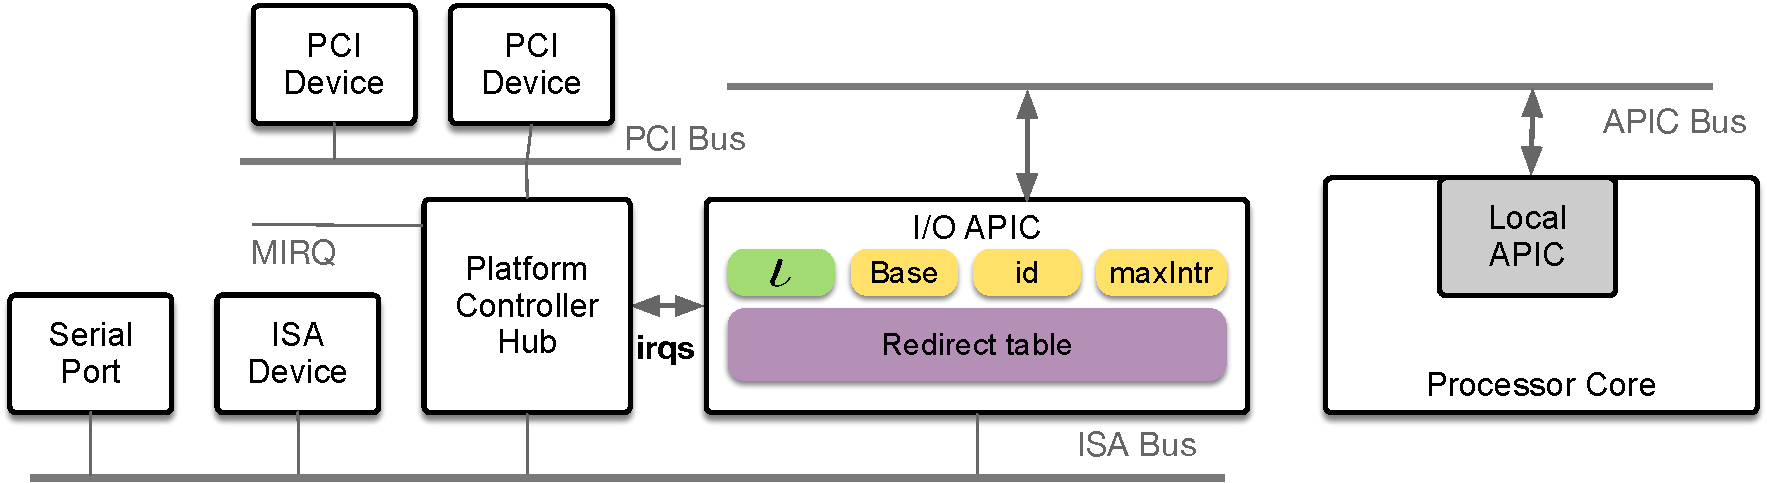
\includegraphics[scale=0.35]{figs/ioapic}
	\end{center}
	\caption{The hardware connections and registers of APIC}
	\label{fig:ioapic}
\end{figure}

\begin{figure}
	\begin{center}
	\[
	\begin{array}{lll}
	s = ( & \iota: \textsf{option} (\mathbb{Z} \times \mathbb{Z}), & \vartriangleright \textit{Current raised IRQ} \\
	& \textsf{id}: \mathbb{Z}, & \vartriangleright \textit{I/O APIC ID} \\
	& \textsf{maxIntr}: \mathbb{Z}, & \vartriangleright \textit{Max redirection entries} \\
	& \textsf{irqs}: \textsf{list} ~ \mathbb{Z}, & \vartriangleright \textit{Redirected IRQs} \\
	& \textsf{masks}: \textsf{list} ~ \textsf{TMask}, & \vartriangleright \textit{Interrupt line masks} \\
	& \textsf{dests}: \textsf{list} ~ \mathbb{Z}). & \vartriangleright \textit{Destinations in Local APIC ID} \\
	\end{array}
	\]
	\end{center}
	\caption{Internal states of I/O APIC}
	\label{fig:ioapic-states}
\end{figure}
%%%%%%%%%%%%%%%%%%%%%%%%%%%%%%%%%%%%%%%%%%%%%%%%%%%%%%%%%%%%%%%%%%%%%%%%%%%%%

\ignore{
The proof is achieved semi-automatically using the big-step semantics of the
CompCert Clight language. The automation is achieved through Coq tactic
libraries including the verification condition generator, arithmetic solvers,
various theory solvers (partial map, list, {\it etc}), and a number of domain
specific libraries which handle items such as device transitions and logs.  The
entire automation libraries are implemented in Coq's tactical language Ltac.
}

\subsection{I/O APIC}

An I/O APIC device collects interrupts from externally connected devices and
distributes them to the corresponding Local APIC. It can be programmed to mask
one or more of these interrupt lines if the OS does not wish to receive
interrupts from some device(s).

Fig.~\ref{fig:ioapic} illustrates the registers and connections of an I/O APIC
device, which collects the IRQs from devices and route them to the Local APIC
controller on CPU. The ``redirect table'' controls the mapping between interrupt
lines and the IRQ number. Following our minimalistic approach, we omit logical
destination, remote-IRR configuration, and other features that are not used in
our kernel. The internal state of the I/O APIC is defined in
Fig.~\ref{fig:ioapic-states}, where $\iota$ represents the interrupt request
currently being processed and its corresponding destination LAPIC ID.

As an interrupt controller, the I/O APIC is treated as a special device. It does
not observe any event from the external environment and thus has neither a
local log nor an environmental transition $\delta^{\textsf{env}}$, but instead,
it receives interrupt requests from the devices and EOI signals from the Local
APIC. We have introduced a special transition function $\delta^{intr}$ to
specify these interrupt-related behaviors.  Accordingly, $\delta^{intr}$ takes
two kinds of events: $\textsf{IRQ} ~ n$ indicates that an IRQ with number $n$ is
triggered by a device; $\textsf{EOI}$ states that the latest interrupt
request has been handled by the OS.  The interesting parts of the transition
rules for $\delta^{intr}$ are shown in Fig.~\ref{fig:ioapic-transition}.

%%%%% Should we explain these rules? 

\begin{figure}
\begin{center}
\[\begin{array}{cr}
	\inferrule{
		s.\iota = \textsf{None} \\
		w = \textsf{IRQ} ~ n \\
		s.\textsf{irqs}[n] = q \\\\
		s.\textsf{masks}[n] = \textsf{Unmasked} \\
		s.\textsf{dests}[n] = d 
	}{
		\delta^{intr}(s, w) \defeq s[\iota \leftarrow \textsf{Some} ~ (q, d)] } & \text{(delivered)} \\[5ex]

	\inferrule{
		s.\iota = \textsf{None} \\
		w = \textsf{IRQ} ~ n \\
		s.\textsf{masks}[n] = \textsf{Masked} 
	}{
	\delta^{intr}(s, w) \defeq s 
} & \text{(masked)} \\[5ex]

\inferrule{
	s.\iota = \textsf{Some} (q, d) \\
	w = \textsf{EOI} \\
	s.\textsf{irqs}[n] = q \\
	s.\textsf{dests}[n] = d 
}{
\delta^{intr}(s, w) \defeq s[\iota \leftarrow \textsf{None}] 
} & \text{(EOI)} 
\end{array}
\]
	\end{center}
	\caption{I/O APIC transition rules}
	\label{fig:ioapic-transition}
\end{figure}

\begin{figure}
	\lstinputlisting [language=C, multicols=2] {src/ioapic.c}
	\caption{The implementation of \texttt{ioapic\_init} in C}
	\label{fig:ioapic_init}
\end{figure}

In addition to $\delta^{intr}$, the I/O APIC also contains the CPU transition
function $\delta^{\textsf{CPU}}$ used to specify the read/write primitives of
I/O APIC, discussed in Sec.~\ref{sec:model}.

In order to coordinate the IRQs assigned by the kernel with the external
interrupt vector, a kernel usually utilizes the Global System Interrupt (GSI)
number. Thus, the IC is first extended into a device object with this extra data
as part of its internal state. Then this IC object is further extended into more
abstract objects by introducing additional driver layers.

At the top level, the I/O APIC device object provides four primitives, two of
them are used to set up the IRQ mappings in the I/O APIC.  Specifically,
\texttt{ioapic\_init} initializes the device when the kernel boots and
\texttt{ioapic\_enable} links a given interrupt line to a Local APIC when a new
device is plugged in or some device changes its working mode. Another two,
namely \texttt{ioapic\_mask} and \texttt{ioapic\_unmask}, are used to enable and
disable a certain interrupt line.

Function \texttt{ioapic\_init} in Fig.~\ref{fig:ioapic_init} shows the
initialization of the I/O APIC. It first reads the size of the interrupt
redirection table (line 2), and for each entry, marks the corresponding
interrupt to be edge-triggered, active high, and masked (i.e. not routed to any
Local APIC). The behavior of this function can be described using the following
rule:
\[
\inferrule{
	l = s.\mathsf{maxIntr} \\
	s' = s[\mathsf{masks}[1 .. l] \leftarrow \textsf{Masked}] \\ 
	s'' = s'[\mathsf{irqs}[1 .. l] \leftarrow \textsf{gsi} .. (\textsf{gsi}+l)][\mathsf{dest}[1 .. l] \leftarrow 0][\iota \leftarrow (\textsf{None}, \textsf{None})] \\
}{
	\texttt{ioapic\_init} (s) = s''
}
\]

Function \texttt{ioapic\_mask} in Fig.~\ref{fig:ioapic_init} shows the code for
masking interrupt line $n$. It first reads the entry `$n-\mathsf{gsi}$' in the
interrupt redirection table (line 13), sets the mask bit (line 14), and then
writes it back to the redirection table. The behavior can be described using the
following rule:
\[
\inferrule{
	\mathsf{gsi} \le n \le \mathsf{gsi} + s.\mathsf{maxIntr} \\ 
	s' = s[\mathsf{masks}[n - \mathsf{gsi}] \leftarrow \textsf{Masked}] \\
}{
	\texttt{ioapic\_mask} (s, n) = s'
}
\]

\subsection{Local APIC}

\begin{figure}
	\begin{center}
		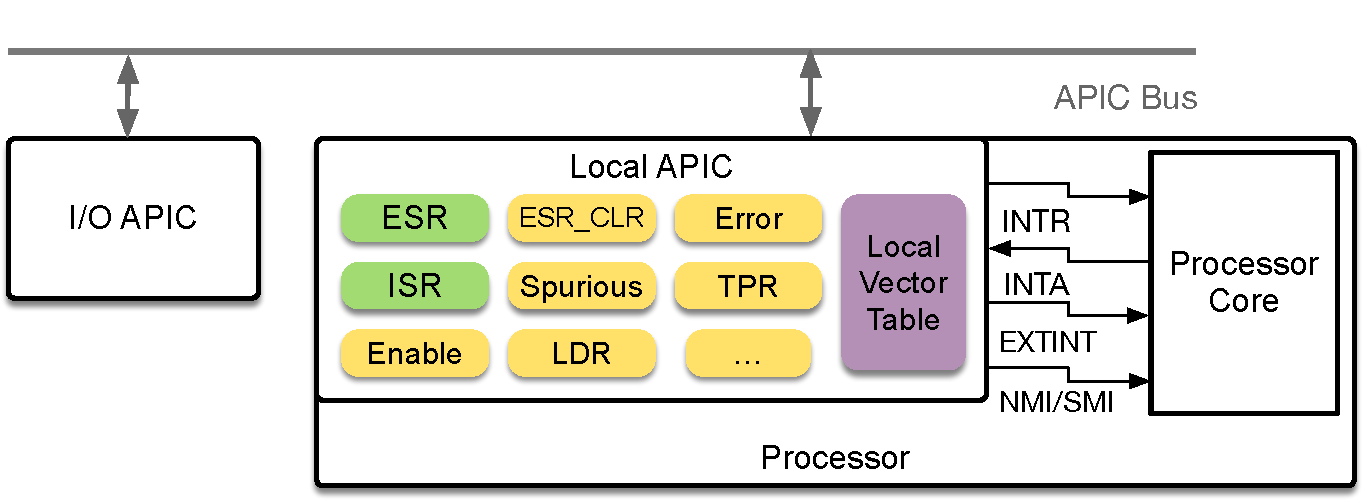
\includegraphics[scale=0.4]{figs/lapic}
	\end{center}
	\caption{The hardware connections of a Local APIC}
	\label{fig:lapic}
\end{figure}

Each processor has a Local APIC device which manages and delivers the interrupt
requests dedicated to this core. It serves as a bridge between I/O APIC and the
processor core and is also programmable which can be used to specify the manner
for each type of interrupt. As shown in Fig.~\ref{fig:lapic}, the Local APIC in
our kernel is mainly served to deliver the external interrupt and generate the
End-of-Interrupt (EOI) signals. An EOI signal indicates current interrupt is
completely handled so that the I/O APIC can issue the next interrupt.

\begin{figure}
	\begin{center}
		\[
		\begin{array}{lll}
		s = ( & \mathsf{ISR}: \textsf{option} (\textsf{IntType} \times \mathbb{Z}), & \vartriangleright \textit{Current in-service IRQ} \\
		& \textsf{ESR}: \mathbb{Z}, & \vartriangleright \textit{Error status register} \\
		& \textsf{ESR\_CLR}: \mathbb{Z}, & \vartriangleright \textit{ESR back-to-back clear ready} \\
		& \textsf{Enable}: \mathbb{B}, & \vartriangleright \textit{Local APIC enable} \\
		& \textsf{Spurious}: \mathbb{Z}, & \vartriangleright \textit{Spurious interrupt vector} \\
		& \textsf{Timer}: \textsf{LvtEntry}, & \vartriangleright \textit{Interrupt control of timer} \\
		& \textsf{Lint~0}: \textsf{LvtEntry}, & \vartriangleright \textit{Interrupt control of local connected I/O devices on line 0} \\
		& \textsf{Lint~1}: \textsf{LvtEntry}, & \vartriangleright \textit{Interrupt control of local connected I/O devices on line 1} \\
		& \textsf{PCint}: \textsf{LvtEntry}, & \vartriangleright \textit{Interrupt control of performance counter} \\
		& \textsf{Error}: \textsf{LvtEntry}, & \vartriangleright \textit{Interrupt control of APIC internal error} \\
		& \textsf{LDR}: \mathbb{Z}, & \vartriangleright \textit{Logical destination register} \\
		& \textsf{TPR}: \mathbb{Z} \times \mathbb{Z}). & \vartriangleright \textit{Task priority register} \\
		\end{array}
		\]
	\end{center}
	\caption{Internal states of Local APIC}
	\label{fig:lapic-states}
\end{figure}

The internal state of the Local APIC is defined in Fig.~\ref{fig:lapic-states},
where \textsf{ISR} represents the IRQ which is being handled. It is set to
\textsf{None} if the CPU is available for incoming interrupts. Following the
minimalistic approach, we omit the features that are not used in our kernel,
such as performance monitoring counters and prioritizer. Other fields in the
Local APIC device object have structure and meaning as in the hardware
specification manual.

\begin{figure}
	\begin{center}
		\[\begin{array}{cr}
		\inferrule{
			s.\mathsf{ISR} = \textsf{None} \\
			s.\mathsf{Enable} = \textsf{true} \\
			s.\mathsf{TPR} = (0, 0) \\
			w = (\textsf{IoAPIC}, n) \\
		}{
			\delta^{intr}(s, w) \defeq s[\mathsf{ISR} \leftarrow (\textsf{ExtInt}, n)][\mathsf{ESR\_CLR} \leftarrow \textsf{false}] \\ } & \text{(ioapic\_delivered)} \\[5ex]
		
		\inferrule{
			o = \textsf{output}~n, v \\
			n = 44 \\
			v = 0 \\
			s.\mathsf{Enable} = \textsf{true} \\
		}{
			\delta^{\textsf{CPU}}(s, o) \defeq s[\mathsf{ISR} \leftarrow \textsf{None}][\mathsf{ESR\_CLR} \leftarrow \textsf{false}]
		} & \text{(EOI)} 
		\end{array}
		\]
	\end{center}
	\caption{Local APIC transition rules}
	\label{fig:lapic-transition}
\end{figure}

Fig.~\ref{fig:lapic-transition} presents some transition rules in Local APIC.
The first rule shows a successful delivery of external IRQ from I/O APIC if
there is no interrupt in service. The second rule shows the transition of EOI in
the Local APIC side, where 44 is the offset to access EOI in the memory mapped
registers. Note that the models of I/O APIC and Local APIC can be merged into a
heterogeneous interrupt controller with the simplified transition rules that are
presented in Sec.~\ref{sec:driver}.



  % Case study
\section{Coq Implementation of Certified Abstraction Layers}
\label{sec:layers}

In this section, we present in detail the actual implementation of the
certified abstraction layers. To make it more easy to reproduce our work,
various examples in this sections are presented directly as they are
implemented in the Coq proof assistant. Various Coq constructions commonly
used throughout this section is presented in Table \ref{table:coq}.
We also explain them as they show up in the examples.

Starting from a bottom-most layer interface abstracting the CPU, device
models and external interfaces, we gradually introduce driver code modules
to develop certified abstraction layers by introducing higher level layer
interfaces abstracting the concrete driver behaviors, and showing contextual
refinement between each overlay interface and the code module running on
the underlay interface, for each of two adjacent layer interfaces.
More formally, for each layer interface $L_{low}$, we introduce a device driver module
$M$, and a new overlay interface $L_{high}$ abstracting the behaviors of $M$, and
show that $\llbracket{}M\rrbracket{}L_{low}$, is
a {\em contextual refinement} of the overlay interface $L_{high}$.
By repeating this strategy, we have developed a stack of layer interfaces,
with the top-most layer interface containing the full abstract behaviors of
the verified device drivers. Next, we introduce these layer interfaces and
the verified driver modules one by one. The implementations of various
concepts in Coq is shown in Fig.~\ref{fig:device:model}, with the concrete
examples used in the rest of the sections listed on the right-hand side.
We explain the concepts and implementations in more detail as we get to the
corresponding layer implementation.

\ignore{
A device layer stack is similar to the kernel layer stack (described in section \ref{sec:preli}) with the following
extensions: 1) Additional abstract states at the machine level (most bottom
layer) which corresponds to the device states. 2) Local logs to record the past
external events. 3) Raw primitives (\textsf{read} and \textsf{write}) for
modeling device access operational semantics.
}

\begin{figure}
\begin{small}
	\[
	{
	\begin{tabu}[t]{l rll l}
%		{\centering \text{Type}}	&	\multicolumn{3}{c }{\centering \text{Definition}}	&	{\centering \text{Coq Presentation}} \\
%s		\hline	
		\textit{Event}	&	E	&	\in	&	\textsf{Recv}~(s:\textsf{list}~\textsf{char}) | \cdots	&	\texttt{Recv str / SendingCompAck / } \cdots \\
		\textit{Log}		&	\ell&	\in	&	\textsf{list}~\textit{Event}	&	\texttt{s.ltx / s.lrx / ...} \\
		\textit{EnvLog}	&	\ell^{\textsf{env}}&:& \text{All possible list of events.} & \text{Build into the `\textsf{next}' function.}\\
		\textit{ident}	&	id	&	\in	&	\textit{Nat} &  \texttt{Let serial\_init := 5950.}\\
		\textit{val}		&	v	&	:=	&	\textit{Vint}~v | ... | \textit{Vundef} & \texttt{Vint v / Vundef / ...}\\
		\textit{Abs}		&	s	&	\in	&	\textit{Type} \times L^{k}	&	\texttt{serial / ioapic / ...} \\
		\textit{Primitive}&	p	&	\in	&	\textsf{list}~\textit{val} \shortrightarrow \textit{Abs} \shortrightarrow L \shortrightarrow \textit{val} \shortrightarrow \textit{Abs} \shortrightarrow \textit{Prop}	&	\texttt{Function serial\_putc\_spec ...}	\\
		\textit{Invariant}&	\textsf{INV}	&	\in	&	\textit{Abs} \rightarrow \textsf{Prop} & \texttt{valid\_cons\_buf\_length: ...}\\
		\textit{Impl}&	\kappa	&:&	\multicolumn{2}{l }{\text{LAsm instruction list or ClightX function.}}  \\
		\textit{LayerIf}&	L	&	\in	& (ident \shortrightarrow Primitive)^{*}	& 
		\begin{tabu}{l}
		\texttt{Definition dserial :=}\\
		\quad \texttt{serial\_init} \mapsto \texttt{serial\_init\_spec}\\
		\quad \oplus~ ...
		\end{tabu}\\
		\textit{Module}&	M	&	\in	& (ident \shortrightarrow Impl)^{*}	& 
		\begin{tabu}{l}
		\texttt{Definition DSerial\_module :=}\\
		\quad \texttt{serial\_init} \mapsto \texttt{f\_serial\_init}\\
		\quad :: ~ ...
		\end{tabu}
	\end{tabu}
	}
	\]
	\vspace{-10pt}
	\caption{The formal model and Coq presentation of device abstract states and layer interfaces}
	\label{fig:device:model}
	\end{small}
\end{figure}

\begin{table}
	\begin{tabular}[t]{p{.3\textwidth}p{.6\textwidth}}
	\hline
		{\centering Statement}	&	{\centering Description} \\
	\hline
		\texttt{x: T}					&	The type of \texttt{x} is \texttt{T}.\\
		\texttt{A -> B}					& 	Arrow type. Non-dependent product.\\
		\texttt{option \_}				&	Option type, either `Some v' or `None'.\\
		\texttt{hd :: tl}				&	List construction. Create a new list with an element `hd' and an old list `tl'.\\
		\texttt{l1 ++ l2}				& 	List concatenation. Create a new list with \texttt{l1} followed by \texttt{l2}.\\
		\texttt{s \{f: v\}}				&	Field update. Replace the value of field `f' in `s' with `v'. \\
		\texttt{Definition x: X := t.}	&	Constant definition. \\
		\parbox[t]{.3\textwidth}{\texttt{Function x ($a_1$:$T_1$)($a_2$:$T_2$)}\\
		\texttt{\hphantom{Func} ... : (rv: T) := $t$.}}
		 & Function definition with arguments $a_1, a_2, \cdots$, return value $rv$ and function body $t$.\\
		 \parbox[t]{.3\textwidth}{\texttt{Fixpoint x ($a_1$:$T_1$)($a_2$:$T_2$)}\\
		 \texttt{\hphantom{Fixp} ... : (rv: T) := $t$.}}
		 & As for function definition but $t$ can make recursive calls to x. \\
		\texttt{match t with} $p_1$ => $t_1$ | ...	\texttt{end}	&	Pattern matching, select $t_1$ if t matches with $p_1$.\\
		\texttt{if b then t else u}		&	Binary selection, b can be either \texttt{true} or \texttt{false}.\\
		\texttt{let x := $t$ in $u$}	&	Local binding.\\
		\hline
	\end{tabular}
	\caption{Common Coq terms, keywords and definitions}
	\label{table:coq}
\end{table}


Traditionally, refinement is proven by an upward simulation from implementation
to specification to ensure soundness, i.e., any property we prove on the overlay
specification is guaranteed to hold at the underlay implementation. In our framework,
we also prove the upward simulation. But as a proof technique, we first prove the
downward simulation and later turn it into an upward one using the fact that our
machine semantics is deterministic with respect to the external events. We model
all non-deterministic behaviors by encapsulating all potential non-deterministic aspects
into event logs. And we prove our strong contextual refinement property with respect
to all possible combinations of event logs. This is how we guarantee
that our proof holds for all possible scenarios in the non-deterministic
executions. 

On the other hand, if the number of simulating underlay steps is not constrained, a
downward simulation could potentially be fulfilled by bogus implementations,  
We always insist writing the deep specifications for the overlay interface to
capture everything contextually observable for the underlay implementation.
Thus, the form of our high-level specifications at overlay is not some random
high-level relations vaguely restricting our underlay behaviors, but actual
precise specifications of what should be the exact outcome after running
corresponding abstract primitive explained in terms of abstract states.
Thus, under same preconditions enforced by the primitive specification, the
behavior of overlay primitive and underlay implementation should be exactly
the same over the same external events. 

\subsection{The Lowest Level Layer Interface: MBoot}

The interface MBoot is the bottom-most layer interface used to model the
behaviors of the CPU and devices. In addition to the abstract states and
primitives in the original verified mCertiKOS, we have extended MBoot with the
new abstract states and read/write primitives for the serial port, I/O APIC, and
Local APIC devices as described in Sec.~\ref{sec:case_study}.

This layer interface introduces a set of layer invariants to enforce the
validity of various hardware states, and all the read/write primitives of the
devices are required to preserve the invariants. In the rest of the invariant
definitions, $\textsf{nth}$ is a list operation defined in Coq, which takes a
natural number $n$, a list $l$, a default value $v$, and returns the $n$'th
value in the list $l$. In the case when the index is invalid, it returns the
default value $v$. $\textsf{nth\_error}$ is a similar operation but returns
either a value or $\textsf{none}$ in the case of an invalid index, instead of
returning the default value. $\textsf{Zlength}$ is another list operation that
returns the length of the provided list as an integer.

\begin{invariant}[valid serial port]
The base address of the I/O port to access \textsf{COM1} is always
\texttt{0x3F8} (1016 in decimal) and cannot be changed by any primitive.
\begin{align*}
serial.\textsf{Base} = 1016
\end{align*}
\noindent{}\textnormal{The primitives \textsf{serial\_read} and
	\textsf{serial\_write} use $serial.\textsf{Base}$ to map the I/O address to the
	registers. Requiring this value to be constant ensures that there is no misuse
	of I/O addresses.}
\end{invariant}

\begin{invariant}[valid I/O APIC maxIntr]
The number of entries in the redirection table of an I/O APIC is less than 239.
\begin{align*}
0 \leq ioapic.\textsf{maxIntr} < 239
\end{align*}
\noindent{}\textnormal{The length of the redirection table in an I/O APIC varies
	depending on the hardware implementation. The actual value for a certain I/O
	APIC is static and stored in the I/O APIC Version Register[16:23], which
	corresponds to $ioapic.\textsf{maxIntr}$ in our device model. This invariant
	guarantees that the actual value of $ioapic.\textsf{maxIntr}$ is within a range.
%	It assures that the initialization of I/O APIC initializes
%	all the interrupt lines in the redirection table.
}
\end{invariant}

\begin{invariant}[valid I/O APIC masks length]
	The length of the mask array in an I/O APIC should be exactly $\textsf{maxIntr} + 1$.
\begin{align*}
\textsf{Zlength} (ioapic.\textsf{masks}) = ioapic.\textsf{maxIntr} + 1
\end{align*}
\noindent\textnormal{For the purpose of saving space, the hardware
	implementation of an I/O APIC makes each entry in the redirection table to be a
	64-bit register containing all the configuration items of a certain interrupt
	line, such as rtbl[i][0:7] for interrupt-vector, rtbl[i][8:10] for delivery
	mode, {\it etc}. In our abstract machine model, we extract each configuration
	item from all the entries and combine them into a list. This invariant requires
	the number of masks to be always equal to $\textsf{maxIntr} + 1$.}
\end{invariant}

\begin{invariant}[valid I/O APIC irq length]
	The length of the interrupt-vector in an I/O APIC should be exactly
$\textsf{maxIntr} + 1$.
\begin{align*}
\textsf{Zlength} (ioapic.\textsf{irqs}) = ioapic.\textsf{maxIntr} + 1
\end{align*}
\end{invariant}

\begin{invariant}[valid I/O APIC irq]
	The value of each interrupt-vector in an I/O APIC ranges from \texttt{0x10} to \texttt{0xFE}.
\begin{align*}
\forall n,~ 0 \le n \le ioapic.maxIntr \rightarrow 16 \leq \textsf{nth}~ n~ (ioapic.\textsf{irqs})~ 0 \leq 254
\end{align*}
\noindent\textnormal{The value in the interrupt-vector is the IRQ number raised
	on the connected CPU. This value can be configured during the runtime and
	should be within the specified range.}
\end{invariant}

\begin{invariant}[valid interrupt states]
	If a device is not in the interrupt service mode (the execution is not in the
interrupt handler), the interrupt controller observed by the device should not
be in the interrupt service mode either. The state $in\_intr$ indicates whether
the system is currently handling an interrupt. Note that it will be abstracted
into corresponding logical states in the extended device objects during the
interrupt refinement process to enforce our isolation policy.
\[
\begin{array}{l}
\textsf{in\_intr} = \textsf{false} ~\rightarrow ~(lapic.\textsf{ISR} = \textsf{None} ~\wedge ioapic.\iota = None)
\end{array}
\]
\end{invariant}


\subsection{Layer Interface DConsoleBufferIntro}

On top of the underlay interface MBoot, we introduce and verify the circular
console buffer (for the serial driver) using the strategy illustrated in Chapter~
\ref{chapter:framework}. The layer interface DConsoleBufferIntro
corresponds to the intermediate layer interface $L_{mid}$ in Chapter~
\ref{chapter:framework}. At this layer, we also introduce the following
invariants on the intermediate console buffer (see Fig.~\ref{fig:spec:cons-buf})
at this layer interface. Recall that, by the design of a layer interface, the
invariants are required to hold at every moment of the system execution. Thus,
these invariants can be used as facts in any part of the verification.
Invariants are stronger notions than the preconditions in the specifications,
in the sense that the preconditions need to be validated during the primitive call while the
invariants are guaranteed to hold before and after calling the primitive.

\begin{invariant}[valid console buffer positions]
\begin{align*}
0 \leq d.rpos < \textsf{CB\_SIZE}
\wedge 0 \leq d.wpos < \textsf{CB\_SIZE}
\end{align*}
\end{invariant}

As explained in Chapter~\ref{chapter:framework}, the contextual
refinement from MBoot to DConsoleBufferIntro is achieved relatively easily as
the abstraction in the current layer interface is extremely similar to the
actual implementation. The concrete methodology is illustrated in Sec.
\ref{sec:dserialintro}, with a simpler example.

\subsection{Layer Interface DAbsConsoleBufferIntro}

This layer interface provides the higher level of abstraction of the console
buffer as a Coq list and corresponds to the layer interface $L_{high}$ in
Chapter~\ref{chapter:framework}. Detailed definitions and the refinement
proofs are omitted since they are already presented in Chapter~
\ref{chapter:framework}. This layer interface introduces a new layer
invariant on the abstract console buffer.

\begin{invariant}[valid console buffer length]
\begin{align*}
0 \leq \textsf{Zlength} (serial.cons\_buf) \leq \textsf{CB\_SIZE}
\end{align*}
\end{invariant}

\subsection{Layer Interface DSerialIntro}
\label{sec:dserialintro}

The next three layer interfaces are designated for the verification of serial
driver. On top of the underlay interface DAbsConsoleBufferIntro, we introduce a
global variable $\textsf{serial\_exist}$ of type $\textsf{bool}$ to indicate
whether the serial device is initialized or not and provide a getter and setter
function called \textsf{get\_serial\_exist}, \textsf{set\_serial\_exist},
respectively. Accordingly, in \textsf{DSerialIntro}, we introduce a new abstract
state $\textsf{serial\_exist}: \textsf{bool}$ and two new getter and setter
primitives under the same names.

\ignore{
The layer interface DSerialIntro introduces following simple invariant.

\begin{invariant}[valid serial\_exist]
\begin{align*}
serial.serial\_exist = \textsf{true} ~\vee~ serial.serial\_exist = \textsf{false}
\end{align*}
\end{invariant}
}


\begin{figure}
	\lstinputlisting [language=C, multicols=2] {src/serial_exist.v}
	\caption{The specification and implementation of C function \texttt{set\_serial\_exist}}
	\label{fig:serial-exist}
\end{figure}

As an example, the source code (in C) and the specification (in Coq) of
\textsf{set\_serial\_exist()} are shown in Fig.~\ref{fig:serial-exist}.
Here, \textsf{Abs} is the type of abstract state in this layer interface,
\textsf{v} is the argument of the primitive, and the boolean function
$\textsf{zlt\_le}~a~b~c$ returns true if and only if $a< b\le c$, as
its name suggests. Furthermore, $d\{attr:val\}$ is our own notation
defined in the Coq, which indicates a new abstract states derived
from the original abstract states $d$, where the attribute $attr$ is
replaced by the new value $val$, but otherwise the same as $d$.
Note that the return type of the
specification function is an option type, and the specification gets stuck
(returns \textsf{None}) when the argument is not within the bound of a 32-bit
integer. This is the requirement that any future caller of this primitive needs
to satisfy.

\begin{figure}
	\lstinputlisting [language=Caml] {src/serial_exist_lowspec.v}
	\caption{The low-level specification of C function \texttt{set\_serial\_exist}}
	\label{fig:serial-exist-lowspec}
\end{figure}
 
The function \textsf{set\_serial\_exist} runs on a machine with the
underlay interface, and our goal is to prove the contextual refinement between
the code running on the underlay and the abstract overlay interface
DSerialIntro. The contextual refinement is proven in three steps.

First, we write a separate low-level specification for the C code
\textsf{set\_serial\_exist} with the low-level memory load and store operations
on the underlay interface, as shown in Fig.~\ref{fig:serial-exist-lowspec}.
Here, ``Inductive'' is the Coq keyword used to define a logical predicate
inductively, with the vertical bar ``$|$'' used to separate different cases
that can cause the relation to hold.
Then the inductively defined predicate
$\textsf{set\_serial\_exist\_low\_level\_spec}~ ge~ args~ m~ rval~ m'$
indicates that under the global environment ($ge$) mapping global variable
identifiers to their locations in the (CompCert) memory, given the argument list
$args$, the function changes the memory from $m$ to $m'$ with the return value
$rval$ ($\textsf{Vundef}$ if no return value). $\textsf{Mem.store}$ is an
operation in the CompCert memory model;  it takes the memory writing type, initial
memory to write to, the memory block, block offset, and a value, and returns the
new memory after writing the value on the location represented by the memory
block and offset on the initial memory. As shown in the figure, the
specification has two cases as in the source code, and in fact, it is very close
to the source code. Thus, it is relatively easy to show that the source code
satisfies the low-level specification shown in
Fig.~\ref{fig:serial-exist-lowspec} and the proof can be achieved nearly
automatically by our proof tactics.

Second, we prove a simulation from the low-level specification at the underlay shown
in Fig.~\ref{fig:serial-exist-lowspec} and the overlay specification shown in
Fig.~\ref{fig:serial-exist}, with a refinement relation that trivially maps the
value of the global variable in the memory at underlay to the new abstract state
at overlay. This part of the proof, which we call {\em data abstraction}, can
vary depending on the kind of concrete data structures in memory and the
abstracted states in the overlay interface. In the case of
$\textsf{set\_serial\_exist}$, the proof is very simple given that it is just a
single variable, but in other cases, the proof could be quite complex and we
may need to further split the proof into multiple layers as shown in the example
of the circular console buffer. The benefit is that after the data abstraction,
the modules and layer interfaces built on top of that could benefit greatly from
the simplicity in the abstracted form.

Last, we apply the correctness theorem of our CompCertX compiler to compile the
C source code and its simulation proof from the first step into appropriate form
in LAsm and link it with the simulation proof obtained in the second step, to
derive the desired final contextual refinement theorem. 

\subsection{Layer Interface DSerial}

On top of the underlay layer interface DSerialIntro, we introduce a new layer
interface DSerial to abstract three driver functions for the serial device. They
are \textsf{serial\_init} that initializes the serial device,
\textsf{serial\_getc} and \textsf{serial\_putc} that reads a character from and
writes a character to the serial device, respectively. The implementation of
\textsf{serial\_getc} and \textsf{serial\_putc} were shown in
Fig.~\ref{fig:serial_putc}, and the C source code for \textsf{serial\_init} is
shown in Fig.~\ref{fig:serial_init_c}.

\begin{figure}
	\lstinputlisting [language=C] {src/serial_init.c}
	\caption{The implementation of \texttt{serial\_init} in C}
	\label{fig:serial_init_c}
\end{figure}

\begin{figure}
	\lstinputlisting [language=Caml] {src/serial_putc.v}
	\caption{The specification of \texttt{serial\_putc} in Coq}
	\label{fig:serial_putc_v}
\end{figure}

A new layer invariant is introduced in DSerial to protect the configuration data.

\begin{invariant}[valid serial state]
	After initialization, the control registers in the serial device should
be properly configured.
\[
\begin{array}{ll}
	serial.\textsf{serial\_exist} = \textsf{true}  & ~\rightarrow \\
	& serial.\textsf{Baudrate} = 115200 ~\wedge~
	  serial.\textsf{Databits} = 8 ~\wedge~ \\
	& serial.\textsf{Stopbits} = 1 ~\wedge~ 
	  serial.\textsf{Parity} = \textsf{NoParity} ~\wedge~ \\
	& serial.\textsf{RxIntEnable} = \textsf{true} ~\wedge~ 
	  serial.\textsf{FIFO} = 1 ~\wedge~ \\
	&  serial.\textsf{Modem} = \textsf{DTR} + \textsf{RTS} + \textsf{OUT2}
\end{array}
\]

\end{invariant}

Both \textsf{serial\_getc} and \textsf{serial\_init} do not contain any loops
and are relatively easy to verify. Note that \textsf{serial\_init} detects the
existence of the serial device, sets the proper configuration based on our hardware
connection parameters, and uses \textsf{set\_serial\_exist} to set the abstract
state \textsf{serial\_exist} when the initialization succeeds.

In the rest of this subsection, we present details on the function
\textsf{serial\_putc}. As shown in Fig.~\ref{fig:serial_putc}, the
implementation of \textsf{serial\_putc} involves a loop to poll the status of
TxBuf (through the \textsf{serial\_read} primitive of the serial device) until it is
empty or reaches the maximum waiting steps. We assume the correctness of
hardware. Thus, we have a separate assumption on the event log stating the TxBuf
always become empty before the maximum iteration is reached.

The specification of the abstract \textsf{serial\_putc} primitive at the new
DSerial layer interface puts the sending character into the serial device's
TxBuf and updates the local log accordingly, as shown in
Fig.~\ref{fig:serial_putc_v}. It first performs some validation checks, including
whether the current execution status is in the critical mode, whether the serial
device is initialized (line 4) and whether the device is properly configured
(line 7). Then, it cases on whether the transmission buffer (TxBuf) is empty
(line 8). Here, we use the notation $d.attr$ to indicate the attribute
value with name $attr$ in the abstract state $d$, and $Z.eq\_dec$ is the
boolean function for integer equality.

Empty buffer indicates that the device is ready to send more characters, and in
this case, the primitive writes the proper contents to the abstract hardware
buffer. Our serial communication protocol requires a new line
(`\texttt{\textbackslash n}') to be a sequence of \textsf{LF} and \textsf{CR}, to
be compatible with most serial applications. The `if' expression at line 10 and
14 serves for this purpose. The local log $\ell_{tx}$  only records the
transmitting events, which separates from the receiving log $\ell_{rx}$. Since we
only consumed a single \textsf{SendingCompAck} event in this case, we simply
fetch the next transmitting event from the environment log ($\ell^{env}$) and
update the transmitting log. Recall that function $\textsf{next}$ is defined in
the Sec.~\ref{sec:model}. It takes a local log, finds the first relevant event
with respect to this log and returns a pair of the event and the updated log.

When the buffer is non-empty, the device is still in the middle of transmitting
messages and the execution needs to wait until the transmission is complete. In
the implementation, there is a loop to poll the status of the transmitter, but
the specification simply writes the TxBuf with the sending message and updates
the log $\ell_{tx}$ to find the first \textsf{SendingCompAck} event in
$\ell^{env}$. This is achieved through the \textsf{next\_sendcomplete} fix-point
function shown in Fig.~\ref{fig:next_complete}. Note that
$\textsf{nextk}~\ell~k$ is a function to call $\textsf{next}$ $k$ times and only
returns the updated log.

\begin{figure}
	\lstinputlisting [language=Caml, multicols=2] {src/next_complete.v}
	\caption{The specification of \texttt{next\_sendcomplete} in Coq}
	\label{fig:next_complete}
\end{figure}

Next, we need to prove the contextual refinement between the specification and
the C code. To do that, we need to design a loop invariant that allows us to
prove that once the loop terminates, the transmission buffer (TxBuf) is empty so
that sending new messages to the serial will not overwrite the previous
messages. Recall that because of our assumption on the correctness of the
hardware, there is always an index $t$ between $0$ and $12800$, at which
iteration the loop terminates and the serial device gets ready for the next write.
Thus, we have designed the following loop invariant:
\[
\begin{array}{l}
(0 \le i \le t ~\wedge~ serial_i = serial_0[\ell_{tx} \leftarrow \textsf{nextk}~ (serial_0.\ell_{tx},~~ i)] ~\wedge~ \textsf{lsr} = 0) ~\vee~ \\
(i = t + 1 ~\wedge~ serial_i = serial_0[\ell_{tx} \leftarrow \textsf{nextk}~ (serial_0.\ell_{tx}, ~~t + 1)][\textsf{TxBuf} \leftarrow nil] ~\wedge~ \textsf{lsr} = 1).
\end{array}
\]

Here, $serial_i$ indicates the value of the abstract state $serial$ after the
$i^{th}$ iteration of the loop, where $serial_0$ indicates the initial state
before entering the loop.
With this loop invariant, the proof can be achieved with the help of
our automation tactic libraries.




\subsection{Layer Interface DConsole}

\begin{figure}
	\lstinputlisting [language=C, multicols=2] {src/cons_intr.c}
	\caption{The implementation of \texttt{serial\_intr\_handler} and \texttt{cons\_init} in C}
	\label{fig:console_c}
\end{figure}

\begin{figure}
	\lstinputlisting [language=Caml] {src/cons_intr.v}
	\caption{The specification of \texttt{serial\_intr\_handler} in Coq}
	\label{fig:cons_intr_v}
\end{figure}

The layer interface DConsole introduces two new primitives. One is
\textsf{cons\_init} which initializes the serial and the console buffer. The
other is the interrupt handler of the serial device
\textsf{serial\_intr\_handler}. Their C implementations are shown in
Fig.~\ref{fig:console_c}.

Once an interrupt signal is produced by the serial device indicating we have
newly received characters in the receiving buffer (RxBuf), the interrupt handler
repeatedly reads the characters one by one from RxBuf and writes them to the
console buffer until either all characters are received or the console buffer is
full of the newly received messages. It is achieved by repeatedly calling the
\textsf{serial\_getc} primitive (introduced at the DSerial) within a loop.

The specification of the \textsf{serial\_intr\_handler} primitive is shown in
Fig.~\ref{fig:cons_intr_v}. In contrast to the C implementation in
Fig.~\ref{fig:console_c}, the specification in Fig.~\ref{fig:cons_intr_v} does
not involve any fix points, but simply concatenates the whole receiving buffer
(RxBuf) into the abstract console buffer list, skipping extra characters in the
head of the list if necessary. This discrepancy between the implementation and
the clean loop-free specification introduces extra complexity in proving the
simulation between those two.

To prove the simulation between them, we first introduce a specification for the
loop and prove the loop body refines this specification. This is used later to
prove the whole function body containing the loop. The specification for the
loop body is a predicate on the abstract state $serial$ and the local
environment for storing the temporary variables in Clight, before ($serial, le$)
and after ($serial', le'$) the loop:
\[
\begin{array}{l}
	serial.\textsf{serial\_exist} = \textsf{true} \rightarrow \\
	serial.\textsf{RxBuf} = str \rightarrow \\
	\textsf{Forall}~~ \textsf{isChar}~~ str \rightarrow \\
	serial.(\textsf{cons\_buf}) = \mathsf{cons\_buf\_mid}~ str~ serial.(\textsf{cons\_buf})~ 0 \rightarrow \\
	le[\textsf{hasMore}] = \textsf{true} \rightarrow \\
	le[\textsf{t}] = 1 \rightarrow \\
	(serial'.lrx = \textsf{nextk} ~(serial.lrx, ~\textsf{Zlength} (tl~ str) * 2 + 1) \wedge \\
	 ~serial'.\textsf{cons\_buf} = \textsf{cons\_buf\_mid}~ str~ serial.\textsf{\textsf{cons\_buf}}~ (\textsf{Zlength}~ str)),
\end{array}
\]

\noindent{}where, $tl$ is the standard list operation that retrieves the tail of
a list, \textsf{Forall  isChar} is an inductive predicate to describe the
property that every character in $str$ is a valid character ($\textsf{fun}~x
\rightarrow 0 \le x \le 255$), and $\textsf{cons\_buf\_mid}~ str~ cb~ n$ is a
function shown in Fig.~\ref{fig:cons_buf_mid_v}. This function calculates the
console buffer when the first $n+1$ characters in $str$ are moved to $cb$.

\begin{figure}
	\lstinputlisting [language=Caml] {src/cons_buf_mid.v}
	\caption{The specification of \texttt{cons\_buf\_mid} in Coq}
	\label{fig:cons_buf_mid_v}
\end{figure}

The loop invariant is constructed as:

\[
\begin{array}{l}
	(~~0 \le i \le \textsf{Zlength} (tl~ str)~\wedge~
	le[\textsf{hasMore}] = 1 ~\wedge \\
	~~~serial_{i}.lrx = \textsf{nextk}~ (serial.lrx, ~~i \times 2) ~\wedge 
	serial_{i}.\textsf{RxBuf} = \textsf{skipn}~(i + 1)~str ~\wedge\\
	~~~serial_{i}.\textsf{cons\_buf} = \textsf{cons\_buf\_mid} ~~str ~~serial.\textsf{cons\_buf} ~~i~~) \\
	\vee \\
	(~~~i = \textsf{Zlength}~ str ~\wedge
	~le[\textsf{hasMore}] = 0 ~\wedge \\
	~~~serial_{i}.lrx = \textsf{nextk} ~(serial.lrx, ~~(\textsf{Zlength}~ str) \times 2 + 1) ~\wedge
	serial_{i}.\textsf{RxBuf} = nil ~\wedge \\
	~~~serial_{i}.\textsf{cons\_buf} = \textsf{cons\_buf\_mid}~~ str~~ serial_{i}.\textsf{cons\_buf}~~ (\textsf{Zlength}~ str)~~)
\end{array}
\]

This loop invariant has two parts: the first part shows the states during the
loop; the second part shows the states when the loop terminates.

\subsection{Layer Interface DIOApic}

The layer interface DIOApic is built on top of I/O APIC machine interface. Four
primitives are introduced in DIOApic: \textsf{ioapic\_init},
\textsf{ioapic\_enable}, \textsf{ioapic\_mask}, and \textsf{ioapic\_unmask}.

The function \textsf{ioapic\_init} initializes the I/O APIC device.
Fig.~\ref{fig:ioapic_init} shows the C implementation of this primitive. It
includes a loop of calling \texttt{ioapic\_write()} to set the interrupt vectors
and masks. The specification of this primitive is shown in
Fig.~\ref{fig:ioapic_init_v}, which contains a fix-point to set related states.
In the figure, the abstract state \textsf{init} indicates whether the device has
been properly initialized. Every primitive other than the initialization
primitive has the precondition on the \textsf{init} being \textsf{true}.

To prove the simulation between these two loops, we first prove the refinement
between the loop body and the abstract \texttt{disable\_irq}. Then we prove the
simulation from the loop to the fix-point \textsf{ioapic\_init\_aux} with
following loop invariant:
\[
	0 \le i \le ioapic_{0}.\mathsf{maxIntr} \wedge
	ioapic_{i} = \mathsf{ioapic\_init\_aux} ~~ioapic_{0} ~~(Z.\textsf{to\_nat}~ i)
\]

\noindent{}From this loop invariant, we can show that when the loop
completes, the final state is consistent with the one in the specification.

\begin{figure}
	\lstinputlisting [language=Caml, multicols=2] {src/ioapic_init.v}
	\caption{The specification of \texttt{ioapic\_init} in Coq}
	\label{fig:ioapic_init_v}
\end{figure}

\ignore{
The specification of \textsf{ioapic\_init} carries a fixpoint which makes the
following verification to be more complex. In mCertiKOS, the kernel execution
consists of two stages: the booting stage and the running stage. \hao{please
	give them a good name.} In the booting stage, all the initialization functions
is invoked, and afterwards, the state $init$ in all the machine will turn from
\textsf{false} to \textsf{true}. 
}

We also introduce a new invariant in this layer interface.

\begin{invariant}[valid I/O APIC state]
	After initialization, the value of interrupt vector corresponding to interrupt line $n$ should be equal to $n + \textsf{IRQ0}$ and this interrupt line should be either masked or unmasked.
	\[
	\begin{array}{l}
	init = \textsf{true} \rightarrow \\
	\forall n \in \mathbb{N}, ~ v \in \mathbb{Z},~
	\textsf{nth\_error}~ (ioapic.\textsf{irqs})~ n = value~ v \rightarrow \\
	( v = Z.of\_nat~ n + \textsf{IRQ0}  ~\wedge~ 
	\exists~ b \in \mathbb{B},~ \textsf{nth\_error} (ioapic.\textsf{masks})~ n = value~ b)
	\end{array}
	\]
	\noindent\textnormal{In the mCertiKOS kernel, we allocate sequential entries from
		the interrupt descriptor table (IDT) for the IRQs. The range is from
		\textsf{IRQ0} to $\textsf{IRQ0} + ioapic.\textsf{maxIntr}$. \textsf{IRQ0} is the
		first IRQ number which is also known as the global system interrupt (GSI). The
		initialization sets the correct values of interrupt vectors which match the IDT
		entries so that the correct interrupt handler can be called when an IRQ occurs.
		The mapping from interrupt lines to IRQ numbers is static in mCertiKOS, so this
		invariant protects this mapping on the I/O APIC. }
\end{invariant}

Primitive \textsf{ioapic\_enable} is used to set the routing configuration for
an interrupt line in order to make it ready for serving the incoming interrupts.
The implementation and specification of \textsf{ioapic\_enable} are shown in
Fig.~\ref{fig:ioapic_enable_v}. Because mCertiKOS only uses one mode of the
interrupt delivery, we only check the validity of given parameters of $lapicid$,
$trigger$, and $polarity$, but do not model the functionality of these
parameters in our device. The \textsf{ioapic\_write} primitive also requires
these parameters to contain exactly the same values.

The primitives \textsf{ioapic\_mask} and \textsf{ioapic\_unmask} are used to
mask and unmask a particular interrupt line designated for a device. It is not
allowed to designate a single interrupt line for multiple devices. Thus, the
masking status of each interrupt line could be later abstracted into the
internal state of the corresponding abstract device object to enforce our isolation
policy. The verification of \textsf{ioapic\_mask} and \textsf{ioapic\_unmask}
is similar to that of \textsf{ioapic\_enable}.

The verification of the four functions introduced in DIOApic is reasonably
simple and can be automated using our tactics.

\begin{figure}
	\lstinputlisting [language=c, multicols=2] {src/ioapic_enable.c}
	\caption{The implementation (in C) and specification (in Coq) of \texttt{ioapic\_enable}}
	\label{fig:ioapic_enable_v}
\end{figure}

\subsection{Layer Interface DLApic}

Two primitives are introduced under the layer interface DLApic:
\textsf{lapic\_init} and \textsf{lapic\_eoi}. The verification of
\textsf{lapic\_init} is similar to \textsf{ioapic\_init}. Recall that during the
later contextual refinement of interrupt models, the operations of two interrupt
controllers will be merged and canceled to derive the abstract interrupt model,
where an interrupt triggered by the serial device is only related to the serial
device object and is independent of either of the interrupt controllers or
the CPU.


\subsection{Above DLApic}

Finally, we introduce a new layer interface to introduce the abstract interrupt
model (as shown in Sec. \ref{sec:interrupt}), and more layer interfaces
for the driver-related system calls.




  % Case study
\section{Evaluation and Lessons Learned}
\label{sec:lessons}

\paragraph{What We Have Proved}
The final theorem we proved for our kernel is the contextual refinement
relation between
our lowest level hardware machine model $\texttt{MBoot}$ (which defines
the x86 instructions, the serial device, and the I/O APIC and Local APIC
devices, etc.), and the top level machine $\texttt{mCertiKOS}$ (which
defines the abstract system call interface).  Let
$\sem{\rm{}x86}{\cdot}$ and $\sem{\rm{}mCertiKOS}{\cdot}$ denote the
whole-machine semantics of each machine model, and $K$ denote the
(assembly) source code of mCertiKOS, then the theorem is formalized
as:

\begin{theorem}
 $\forall P,\;\sem{\rm{}x86}{K\join{}P}\Refrel{}\sem{\rm{}mCertiKOS}{P}$.
\end{theorem}

The theorem states that for any kernel/user/guest/host
context program $P$, there is a simulation between program $P$ running
on top of the top level abstract machine $\texttt{mCertiKOS}$, and the
program $P$ linked with the mCertiKOS source code $K$, running
atop the bottom-most machine $\texttt{x86}$.

The abstraction layers also define the data invariants that are proved
to hold at any moment of the whole program execution. Some example
invariants are: the console's circular buffer is always well\-formed,
and the interrupt controller states are always consistent, {\it etc}.

Besides this, our framework automatically derives that all the system
calls always run safely and terminate; there are no code injection
attacks, no buffer overflows, no null pointer access, no integer
overflows, {\it etc}.

\paragraph{Isolation}
We take the existing implementation of the CertiKOS infrastructure
\cite{dscal15}, and extend it with our device and interrupt models.
On top of the extended machine model, we have verified a subset of the
device drivers in mCertiKOS with 10 abstraction layers. Some layers
are introduced to verify concrete driver implementation, while others
are introduced purely for logical abstraction (e.g., from a circular
console buffer implementation in memory to an abstract list, from the
hardware interrupt model to the abstract interrupt model enforcing
isolation, {\it etc}).  These abstraction layers are inserted into the
existing layers of mCertiKOS as a certified plugin.  Thanks to our
isolation policy, this does not invalidate most of the existing proofs
of mCertiKOS, and the integration only required minimal effort, despite
the existing mCertiKOS proofs being unaware of interrupts.


\paragraph{Execution Model and Completeness}
The majority of our device drivers are specified and verified at C
level, then compiled by our CompCertX compiler. 
The entire kernel (both C and assembly)
source code, together with the source code for the verified compiler,
are extracted into an OCaml program through Coq's extraction
mechanism. When this program gets executed, it compiles the extracted
C source code into the assembly, and merges it with the existing
assembly kernel source code, to produce a piece of assembly code
corresponding to our verified kernel.  Thus, our deliverable comes
with a piece of assembly code for the entire verified kernel, a high
level deep specification of various kernel behaviors, and a machine
checkable proof object stating the assembly code running on the actual
hardware satisfies the high level specification.

The verified assembly code is then linked with the rest of kernel code
(the boot loader and remaining unverified drivers) to produce the
actual binary image of the OS. The resulting kernel is practical: it
runs on stock x86 hardware and the hypervisor version with the Intel vt-x
support can successfully boot a unmodified version of Linux as guest.

\paragraph{Verification Effort} 
Using our general device interface, we have modeled a serial device
and two interrupt controller devices. On top of these device models,
we have verified the related drivers and interrupt handlers.  The
entire verification effort consists of roughly 20k lines of Coq code
added to the existing mCertiKOS verification code base.  Regarding the
specification, there are 510 lines of code used to specify the machine
model including the device hardware, and 126 lines of code for
specification of the additional system call interfaces. There are
additional 9,829 lines of Coq code that were used to define auxiliary
definitions, lemmas, theorems, invariants, {\it{}etc}. Note that these
9,829 lines of definitions are outside our TCB, thus does not need
to be trusted.  In terms of proof size, there are 3,671 lines of Coq
code for the layer refinement proofs, 3,589 lines for code
verification, 1,802 lines for proving invariants, and 307 lines for
linking different modules together.

The entire verification effort took roughly 7 person months, the
majority of which went into the design and development of the
framework itself, including the extended machine model, general device
framework, the interrupt refinement, and the tactic libraries for
automating most of the non-intellectual parts of verification task.
We anticipate the cost of verification for future drivers would be
dramatically reduced.

\paragraph{Bugs Found}
An extended version of the mCertiKOS kernel has been deployed in a
practical system that is used in the context of a large DARPA-funded
research project \cite{dscal15}.  Yet, through the verification of the
console driver, we found a critical bug which may lead to the loss of
many characters received from the serial device. The bug was in the
implementation of the circular console buffer, where, in some rare
cases, the read and write positions to the buffer array overlap,
causing the entire contents in the buffer to be lost. The bug was
caught when we tried to establish the contextual refinement between
the concrete implementation of the circular buffer and its abstract
list representation.

Another bug was found in the code for initializing the serial device,
where the interrupt was not configured correctly by accidentally
setting the Interrupt Enable Register (IER) before the DLAB was unset.
This was caught when we tried to prove the initialization code against
its specification.



		 % Evaluation and lessons learned

\chapter{Verification of Concurrent Programs}
\label{chapter:concurrent}

In this chapter, I show how we extend our engine to support
verification of concurrent programs with fine grained locking.
As illustrated in Chapter \ref{chapter:driver}, our definition of
certified abstraction layers do not directly work with concurrent programs,
as the contextual refinement between the specification and implementation
would not hold due to the arbitrary interleaved executions with other
devices/CPUs. This is because the way we specify the function
does not take account the potential change to the (shared) abstract states
and memory due to the interleavings. On the other hand, it is definitely
not practical to encode all possible ways of the state changes from
interleaved executions in the specifications themselves.

Thus, we need a way to effectively represent the shared states among programs
on different CPUs, and the non-deterministic accesses to these shared
states. We would also want to reuse all the techniques
that we have built for verification of sequential programs.
Recall that we have successfully handled some limited form of concurrency
between the devices and a sequential program in Chapter \ref{chapter:driver}.
There, we have developed a new machine model, where the devices are treated
as if they do not execute together with the CPU, and only try to replay
the states of a device when we disable and enable the interrupts on that
device. These two are considered as valid synchronization points because
we do not access the states of the device when the interrupt of the device
is enabled, and we can recompute the current states of the device solely by
applying the device model to the list of external events we observe on that device.

This is clearly restricted to the limited form of concurrency in consideration,
and cannot be directly applied to reasoning of arbitrary concurrent program.
Yet, the general idea is still valid, and we have indeed extended this line of
idea to a concrete framework that is suitable to reason about arbitrary
concurrent programs with fine grained locking in modular ways.
By modular reasoning of concurrent programs, we would expect to reason about
each program running on a CPU or thread separately, by making valid assumptions
to the rest of programs and outside world, and in the end link these individual
proofs formally to reach a final conclusion about the entire program when they
run altogether concurrently. 
In Chapter \ref{chapter:driver}, we still use the abstract states
to model the shared states (the states of devices), which, at synchronization
points, get computed by applying the effect of external events on the current
shared states. Naively applying this would cause the discrepancy when the current
thread uses the abstract states to represent the shares states, while the rest
of the world uses the events. Instead, we always use the list of events to represent
the shared states among threads and processes. In this model, modifying shared
states can be specified simply as appending a new corresponding event to the
event list, and this list can be synchronized by appending the list of events
generated by the rest of the world at every carefully chosen synchronization points.
The the actual shared states can be derived from the list of events by replaying
the effects of the each event in the list from an initial state. We attach such
\emph{replay function} for each shared state and related events.

Recall that in the sequential world, the task of layer based verification is to prove
the contextual refinement between the concrete function implementation manipulating
concrete in-memory data and the abstract high level specification described in
terms of the corresponding abstract states. In this case, the context would be the
user program, other kernel or hypervisor functions, {\it etc}.
In the concurrent world, we also have the programs running on other CPUs/threads,
in parallel with the current function being verified.
Thus, in this case, the task involves proving the contextual refinement between
the function implementation operating on the shared memory and abstract states,
and the abstract high level atomic specification that triggers an atomic high level
event. In the next section, we present this new framework in more detail.

\section{Certified Concurrent Abstraction Layers}

\paragraph{Machine State}
Our new x86 machine state $s$ is a tuple $s~:=~(c, f_p, m, a, l)$.
Here, the component $c$ stands for the current CPU ID, and $f_p$ is
a partial map from a CPU ID to the private states of that CPU.
In addition, $m$ stands for the memory shared across CPUs, and $a$
stands for the shared abstract states. The list $l$ represents
the list of observable global events in the chronological order.
As we mentioned earlier, we represent all shared
states by the list of events, where the concrete states can be reproduced
by applying the replay function to the list of events starting from the initial states.

\paragraph{Transitions}
In the new concurrent machine, a transition may refer to a regular execution
of an assembly instruction, invocation of a private primitive that only changes
CPU local states, or a shared primitive call that could trigger events
observable to other CPUs. To model the non-deterministic execution among
different CPUs, we also have a special transition that changes the current
CPU ID $c$ to some other CPU ID, which we call \emph{hardware scheduling transition}.


\paragraph{Restrictive Memory Model}
Eventually, we would like to prove that every memory access from our entire
verified concurrent program is safe, and there is no data race.
Instead of proving all these desired memory access properties as separate
lemmas for every program, as our usual verification technique, we take a
more systematic approach, i.e., we design a memory model only for safe
memory access such that all the undesired programs semantically get stuck
on our memory model. This ensures that every verified program on our framework
must be data race free.

As a result, in our memory model, we associate every memory block $b$ with
an ownership status in the abstract state $a$, which can only be manipulated
by two new logical abstract primitives \emph{push} and \emph{pull}.
The \emph{pull} operation modifies the ownership status of the memory block
from ``free'' to ``owned by $c$'', while the \emph{push} operation frees back
the ownership of the memory block, together with the updated memory.
These two operations abstract all shared memory access at our
lowest machine model as atomic logical primitives that triggers corresponding
\emph{push} and \emph{pull} events. 
As described above, if a program tries to pull a non-free location, or tries to
access or push to a location that is not owned by the current CPU, the
machine semantics gets stuck. 
This way, we encapsulate every valid shared memory access with corresponding
\emph{push} and \emph{pull} events from involved CPUs.
We show in Section \ref{veri-ticket-lock}
how we can further encapsulate and abstract these logical primitives to
build a spinlock module.


\paragraph{Active CPU Set and Environmental Context}
To enable modular reasoning of concurrent programs, we would like a way
to semantically reason about only part of the whole program locally, by
making reasonable assumptions on the rest of programs, and finally formally
combine the reasoning of these individual programs together, to reach a
final conclusion about the full program.
We call the set of CPUs in consideration the \emph{active CPU set} $A$, and
specify the assumptions over the external world outside $A$ as the
environmental context $\oracle$, which is a partial map from a list of
current global event log $l$ to another list of events $l'$ that corresponds
to the list of observable events triggered by the CPUs outside $A$ at this
interleaving point. We denote such concurrent layer interface $L$ parameterized by
an active CPU set $A$ and environmental context $\oracle$ as
$\PLayer{L}{A}{\oracle}$.

We encode our assumptions on the external world by
enforcing a \emph{Rely} condition on the list of event logs
the environmental context returns,
and represent our own invariants by introducing a \emph{Guarantee} condition
on the list of events triggered by programs running on the active CPU set $A$.
If we have separately verified two sets of concurrent programs running on
a disjoint sets of CPUs $A$ and $B$, and each of the \emph{Guarantee} condition
implies the other's \emph{Rely} condition, then we can merge these two proofs
together to derive a proof on a combined concurrent program running on the
active CPU set $S_{AB}=A\cup B$ and the environmental context 
$\oracle_{AB}=\oracle_A\cap\oracle_B$.
Since the event list $l$ is part of our abstract state, and the list of events
from the environmental context is also appended to $l$, both the \emph{Rely}
and \emph{Guarantee} condition can be represented as regular layer invariants
in our concurrent certified abstraction layer framework.

\ignore{
\paragraph{Concurrent Layer Interface}

Now we define the \emph{concurrent layer interface} $\PLayer{L}{A}{\oracle}$,
parameterized over the active CPU set $A$, and the environmental context
$\oracle$, as a tuple $(\Layer, \Rely, \Guard)$, where the $\Layer$ defines
the abstract states and primitives (similar to the sequential version),
and $\Rely$ and $\Guard$ being the \emph{Rely} and \emph{Guarantee} condition.
}

\paragraph{Building Concurrent Certified Abstraction Layers}
Now we define the contextual refinement in the concurrent setting,
using the definition in the sequential case.

\begin{definition}[Contextual Refinement]
For every code module $M$, active CPU set $A$, and environmental context
$\oracle$, we say $\llbracket{}M\rrbracket{}L_1$ contextually refines
$L_2$ over $A$ and $\oracle$ if and only if there exists a function
$f$ such that $\llbracket{}M\rrbracket{}\PLayer{L_1}{A}{\oracle}$ contextually
refines $\PLayer{L_2}{A}{f(\oracle)}$. 
\end{definition}

Similar to the sequential case, we have developed some proof patterns on
building concurrent certified abstraction layers, layer by layer.
Our verification is still per function basis, and we verify the programs
running on each CPU separately, and build up the standard layer hierarchy
$\PLayer{L}{\{c\}}{\oracle}$ for each CPU $c$. For simplicity, we note this
\emph{CPU local layer} as $\PLayer{L}{c}{\oracle}$.
In the end, we compose these proofs for each CPU
into a combined proof for the whole concurrent program.

We have developed two proof patterns to help building certified concurrent
abstraction layers. First, we use \emph{fun-lift} pattern to abstract shared
physical memory into shared abstract states, and specify and verify the
concurrent functions with these abstract states, in a way very similar to
how we build the sequential layers. Note that this process does not change
any potential interleavings in the programming executions, and each shared
operation is specified by querying the environmental context to obtain the
external event list at every interleaving point, i.e., our primitive specifications
are no longer atomic as their behavior depends on other concurrent programs' behavior
in the middle of the primitive executions. On the other hand, by not handling
the concurrency at this level allows us to be able to reuse most of the
frameworks and techniques we have built for verifying sequential programs.

Once we are at a layer where we have a full behavior of the shared
``atomic'' primitives, we utilize the second \emph{log-lift} pattern to
lift the layer into a new layer where the specifications of the shared
primitives are atomic, i.e., they simply trigger a new single atomic
event. Proving the contextual refinement between these two layers include
the critical concurrency reasoning on the fact that the events can be
shuffled and merged into a new list where we can always map a consecutive
list of underlay events into a single new event at the overlay.
Concretely, we need to find a function $f$ that can transform the environmental
contextual of underlay into one at overlay, and a refinement relation $R$
that matches the underlay and overlay states, especially the two event list
with events generated both locally and returned by the environmental context.
We illustrate this process in more details in the examples in subsequent sections.

\paragraph{Multicore Linking Theorem.}
By composing all the CPUs in the machine (denoted as the set $D$), the resulting 
layer interface does not depend on any environmental events except those
hardware scheduling transitions among different CPUs.
We construct such a layer interface $\PBoot[D]$
using the primitives provided by the layer $\Mach_{\boot}$, which is the lowest
layer that we use to model the multicore hardware environment. 
We can then prove a contextual refinement from  $\Mach_{\boot}$ to $\PBoot[D]$
for every possible interleaved executions.
\begin{theorem}[Multicore Linking]
\label{thm:link}
$\forall P, \sem{\Mach_{\boot}}{P} \refines_R \sem{\PBoot[D]}{P}$
\end{theorem}
This theorem ensures that all code verification over $\PBoot[D]$ can be propagated down to the x86 multicore hardware 
$\Mach_{\boot}$.


\section{Verification of Ticket Lock}
\label{veri-ticket-lock}


\subsection{Spinlocks}
\begin{figure}[t]
\lstinputlisting [language = C] {src/ticket_lock.c}
\caption{Pseudocode of ticket lock implementation.}
\label{fig:exp:real_ticket_lock}
\end{figure}

Spinlocks are one of the most basic synchronization
methods for multicore machines; they are used as building
blocks for shared objects and more sophisticated synchronizations.


A spinlock enforces mutual exclusion by restricting CPU access to
a memory location $b$. Lock operations can be viewed
as ``safe'' versions of $\push/\pull$ primitives.
For example, when the lock acquire  for $b$ succeeds,
the corresponding shared memory is guaranteed
to be ``clean'', meaning that it is safe to 
pull the contents to the local copy at this point.
As an example, Fig.~\ref{fig:exp:real_ticket_lock} shows
an implementation of the ticket lock algorithm \cite{mcs91}.
As can be seen in Fig.~\ref{fig:exp:real_ticket_lock},
the $\acq/\rel$ functions invoke the $\push/\pull$ primitives.
\footnote{Note that even though these primitives are
called in the layer as if they are actual function primitives,
those are only logical primitives that do not intend to incur
any performance overhead, and are only used as a verification
technique.}
We now show how we build concurrent certified abstraction layers
for the ticket lock implementation shown
in Fig.~\ref{fig:exp:real_ticket_lock}.

\noindent\textbf{Step 1 (memory operation interface $L_0$).}
We first develop a layer, where the three tick related primitives
are abstracted into three atomic primitives \texttt{get\_n},
\texttt{inc\_t}, and \texttt{inc\_n}, which generate corresponding
external low level event. Thus, including the events generated by the
\texttt{push} and \texttt{pull} primitives, the external event list
$l$ in the new layer $L_0$ contains the following sets of events:

\[
\begin{array}{c}
\incticket(b) \mid \incnow(b) \mid \getnow(b)
\mid \push(b,bl) \mid \pull(b)
\end{array}
\] 

To reconstruct the value of $t$ and $n$ from events, we define a replay
function $\replay_{\comm{ticket}} : Log \to \integer \to \integer\times \integer$. 
The definition is as one would expect:
$\replay_{\comm{ticket}}(\mathsf{nil}, b) = (0,0)$, and each 
$\incticket(b)$ and $\incnow(b)$ event in the list increments
the first or second component of the pair, and other events are ignored.

The atomic ticket primitives are implemented using the atomic x86 assembly
instructions. For example, we implement the
fetch-and-increment $\mathsf{FAI\_ticket}$ primitive in a small 
assembly snippet, yielding the following specification:

\begin{mathpar}
\inferrule{
 l_0 = l \cons \oracle(l) \\
  \replay_{\comm{ticket}}(l_0, b) = (i,j) \\
  l' = l_0 \cons c.\incticket(b)\\ 
}{
 \oracle, c \vdash  \spec_{\mathsf{FAI\_ticket}}([b], l, i, l')
}
\end{mathpar}

Here, $c.\incticket(b)$ means the event is triggered by the CPU
$c$, and ``$\cons$'' means ``cons-ing'' an event to the log.
The specification $\oracle, c \vdash  \spec_{\mathsf{FAI\_ticket}}([b], l, i, l')$
indicates that the for all possible environmental context $\oracle$ and
CPU ID $c$, the primitives takes an argument $b$ and returns an
integer $i$, transitioning the event log from $l$ to $l'$. Other
irrelevant states are not shown here for simplicity as they do not change
during this transition.

As shown in the specification,
the primitive queries $\oracle$ and appends the result list and
one new event to the log,
then returns the current state $i$ of {\tt ticket} computed by
replaying the result log.
The fact that we are
using an atomic memory instruction, and that such memory updates are
immediately visible to all CPUs, is reflected by the
primitive just adding a single event so there can be no unexpected
interleavings between CPUs. We add similar specifications for the
other operations, \eg, a $\sigma_{\mathsf{get\_now}}$ primitive whose
implementation is a memory read, and whose specification queries
$\oracle$ to get the new log $l_0$, appends $\getnow (b)$, and returns
$\mathsf{snd}(\replay_\mathsf{ticket}(l_0, b))$.
The layer interface $L_0$ is defined as below:

\[
\begin{array}{rl}
L_0 := &\mathsf{FAI\_ticket} \mapsto \spec_{\mathsf{FAI\_ticket}}
\oplus \mathsf{inc\_now} \mapsto \spec_{\mathsf{inc\_now}} \\
&\oplus \mathsf{get\_now} \mapsto \spec_{\mathsf{get\_now}}\oplus  \push\mapsto \spec_{\push}
\oplus  \pull\mapsto \spec_{\pull}
\end{array}
\]

\noindent\textbf{Step 2 (low-level specification $L_1$)}
Next, following the \emph{fun-lift} pattern,
we verify the implementation of the ticket lock shown in 
Fig.~\ref{fig:exp:real_ticket_lock}, on top of the previous
layer interface $L_0$.
As illustrated before, on this pattern, we do not aim to change
any potentially interleavings in the programming executions, and
we specify each shared operation by querying the environmental context
to obtain the external event list at every interleaving point.
To come up with such a specification at $L_1$ for $\rel$ is
straightforward, and it just appends the $\push$ and $\incnow$ events
to the log, while querying $\oracle$ and appending the result
list before it pushes each event to the log, capturing all possible
interleaved executions at each such synchronization point.

However, we need some care to assign a good specification to
$\acq$, as it contains a while-loop. To prove total correctness,
we would like to assign a specification which later can be proven
to terminate.
We define an auxiliary function $\comm{wait}$
(using recursion in Coq) describing the behavior of the first $k$
iterations of the loop: each time we query the environment
context $\oracle$, it generates its own
event, and checks if CPU number $c$ is due to hold the
lock. The function is undefined (Coq {\tt None}) if we do not get the
lock within $k$ iterations.

\[
\begin{array}{lcl}
\mathsf{wait}(0, \oracle, c, b, l) & = &\text{undefined} \\
\mathsf{wait}(k+1, \oracle, c, b, l) & = & l', \text{ if $l'$ indicates next is $c$'s turn to get lock}\\
                       & &   \mathsf{wait}(k, \oracle, c,  (l' \cons c.\getnow(b))), \text{ otherwise} \\
                       & &  \text{where }l' = l \cons  \oracle(l)
\end{array}
\]

We then define the semantics of the primitive by saying that it first
generates an $\incticket$ event, and then loops
for some ``sufficiently'' large number $\calwait(l, c)$ of iterations.

\begin{mathpar}
\inferrule{
  l_0 = \mathsf{wait}(\calwait(l, c), \oracle, c, b,
  	l \cons \oracle(l) \cons c.\incticket(b)) \\
  	l'  = l_0 \cons c.\pull(b) \\
}{
 \oracle, c \vdash  \spec_{\acq\_\mathsf{low}}([b], l, \any, l')
}
\end{mathpar}

Computations where $k$ reaches 0 are considered stuck, and our
ultimate theorem is about safe programs (programs that does not get stuck).
Thus, to prove the \textbf{starvation-freedom} of ticket lock,
we have to know what number $\calwait(l,c)$ is sufficiently large.
We make following two assumptions. Fist, the hardware scheduling transition
is fair, i.e., there exists a number $h$ such that the nondeterministic execution is
guaranteed to get back to the previous CPU within $h$ hardware steps.
Second, every CPU who acquired the ticket lock released the lock within
$r$ steps for some constant $r$. This is also a reasonable assumption because if someone
holding the lock never releases the lock, no one else can ever obtain the lock
again. Both of these assumptions are formally enforced by introducing
them as layer invariants on the event list $l$.
Given these two assumptions, and also assuming there are $n$ number
of CPUs available on the machine, we can conclude that each CPU
needs to wait on the lock for at most $h * r * n$ steps, as even if all
other CPUs were in the queue ahead of the current CPU, they would eventually
all release the lock within these many steps and no one can take the lock
bypassing the currently CPU's turn by definition of the ticket lock.

The main task in proving the contextual refinement between $L_1$ and $L_0$
is to prove that the implementation shown in Fig.~\ref{fig:exp:real_ticket_lock}
satisfies the specifications shown above. The refinement proof is
straightforward because the abstract state and the global log are identical
in both layers, and thus the simulation relation is the identity relation.

On the other hand, in this \emph{fun-lift} pattern, we can reuse all the
techniques we have developed for verification of sequential programs, as
there is no reasoning of interleavings involved here. One technical challenge
apart of concurrency is that the ticket in the specification increases
monotonically, while in the implementation, we have to use finite precision
integers that wraps back to zero when it reaches the maximum. Thus, as you
see in the implementation, we use the $!=$ operator instead of $<=$.
\newman{Add verification details here with concrete invariants}

\vspace{3pt}
\noindent\textbf{Step 3 (atomic specification $L_2$)}
Recall that the specification $\spec_{\acq}$ and $\spec_{\rel}$ in $L_1$
are not atomic, as they involve potential interleavings in the middle
(encoded by querying the environmental oracle for external events).
On the other hand, as clients using the lock, we would treat the lock
primitives as if they were atomic, even in reality, there could be
some irrelevant interleaved executions in the middle.
We achieve this by introducing a new higher layer interface $L_3$ using
the \emph{log-lift} pattern, which contains atomic specifications
for $\acq$ and $\rel$ primitives.

Unlike previous two layers, the new layer $L_3$ does not contain any of
the low level events, but instead contains two new events
$\acq(b)$ and $\rel(b)$. The specifications for the two primitives are
now very simple: they just query the environment context, and then
introduce one more event.

\begin{mathpar}
\inferrule{
    l' = l \cons \oracle(l) \cons c.\acq(b) \\
}{
 \oracle, c \vdash  \spec_{\acq}([b], l,\any, l')
}
\\
\inferrule{
  l' = l \cons \oracle(l) \cons c.\rel (b)
}{
 \oracle, c \vdash  \spec_{\rel}([b], l,\any, l')
}
\end{mathpar}

By having these primitives introduce only a single event, clients of the
lock code can treat the lock operations as completely \emph{atomic}; there is
no need to consider interleavings of the ``get lock'' execution
with events from other CPUs. 

In order to prove the contextual refinement between $L_2$ and $L_3$, we
need to find a function $f$ that can convert $\oracle_2$ to $\oracle_3$,
and also a refinement relation $R$ that 
relates the list of events $l_2$ in $L_2$ to the list $l_3$ in $L_3$.
We map two list of events by mapping $\pull(b)$ in $l_2$ to $\acq(b)$
in $l_3$, and $\incnow(b)$ to $\rel(b)$,respectively, ignoring all other
events in $l_2$. Function $f$ can be derived from this relation by
applying $\oracle_2$ to matching underlay events and converting it to
the list of overlay events following the same conversion rule.
Then we finally prove that the refinement holds for every primitive
over this setting.
This simulation proof is only between specifications, and in the end,
we can compose proofs of individual primitives to derive the full
contextual refinement as in the sequential case.

\paragraph{Extending to Other Type of Spinlocks}
This event-based specification for the spinlock is also general enough
to capture  other implementations like the \emph{MCS Lock},
which is known to have better scalability than ticket lock
over machines with a larger number of CPUs. We have also
implemented a version of MCS locks~\cite{kim2017safety}, following
similar proof technique, while maintaining exactly same high level
specifications for $\acq$ and $\rel$ as in $L_3$ above.


\section{Shared Queue Object}

\begin{figure}[t]
\lstinputlisting [language = C, multicols=2] {src/dequeue.c}
\caption{Pseudocode of dequeue implementation.}
\label{fig:exp:dequeue}
\end{figure}

Given that we have verified ``atomic'' lock acquire and release primitives,
we can utilize these spinlocks to verify more useful concurrent
data structures and programs. Shared queue is one of the widely used
data structures used in concurrent programs like producer/consumer,
scheduler, {\it etc}. 

The specification of a shared queue object should provide a high level abstract
interface by hiding all the low level details,
to ease the verification of programs using the object.
However, the large gap between this high level abstract specification
and the low level efficient implementation makes the verification of the shared queue object
itself extremely challenging.
The previous verification technique for shared queue object~\cite{lili16}
has to inline the lock implementation and duplicate the lock-related proofs, due
to the lack of modular layered approach.

Figure \ref{fig:exp:dequeue} shows the implementation of dequeue operation, where
we represent the queue in terms of a doubly linked list. 
As shown in the figure, we utilize an auxiliary function $\deq\comm{\_t}$ which
performs the actual operations on the queue. The main function $\deq$ simply
wraps $\deq\comm{\_t}$ with the lock acquire and release functions.
To verify this shared queue, we first verify the $\deq\comm{\_t}$ function
via the  \emph{fun-lift} pattern for sequential program, where the specification
assumes that the lock is already held, thus no interleaved executions are possible
in the middle of $\deq\comm{\_t}$. Then we utilize 
the \emph{log-lift} pattern to introduce another layer for the main $\deq$ function
where it simply generate one single $\deq$ event. This can be done by merging two
queue-related lock acquire and release events underlay into a single $\deq$ event
at the overlay. 


\section{Supporting Multiple Virtual Machines}

\subsection{Extending The Single VM Implementation}

\subsection{Verification Challenges}

\section{Evaluation and Experience}
\label{sec:kernel}

\begin{figure*}[t]
\centering
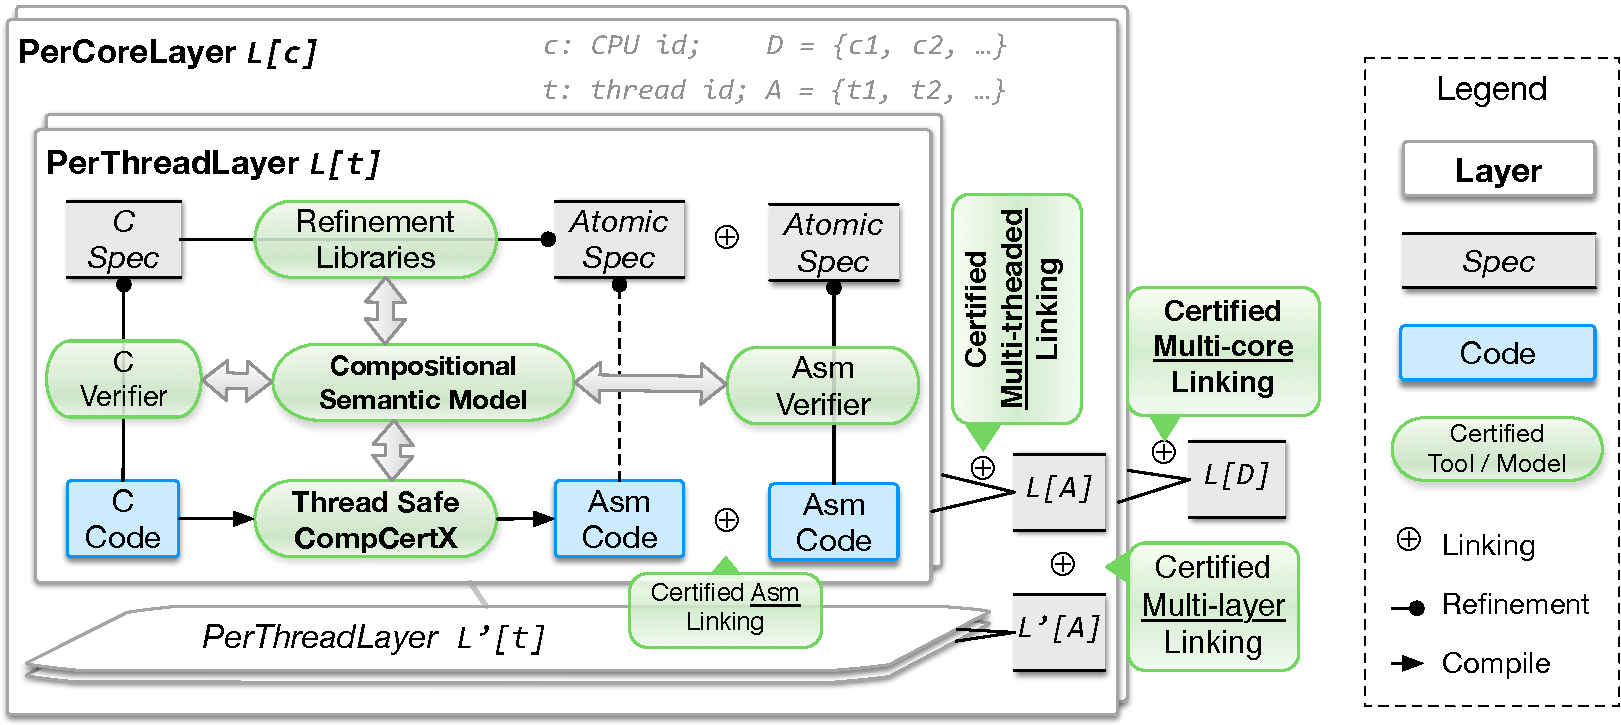
\includegraphics[scale=.45]{figs/tool_chain}
\caption{System architecture of the CCAL programming toolkit.}
\label{fig:toolchain}
\end{figure*}

\begin{table}
\begin{center}
\begin{footnotesize}
\renewcommand{\arraystretch}{1} 
\begin{tabular}{|c|c||c|c|}
\hline
Component & LOC & Component & LOC \\
\hline
\hline
Auxiliary library & 6,200 & Multilayer linking & 17,000 \\
\hline
C verifier & 2,200 & Multithread linking & 10,000 \\
\hline
Asm verifier & 800 & Multicore linking & 7,000 \\
\hline
Simulation library & 1,800 & Thread-safe CompCertX & 7,500\\
\hline
\end{tabular}
\end{footnotesize}
\end{center}
\caption{Lines of proofs in Coq for the toolkit.}
%\hrulefill
\label{table:toolkit}
\end{table}

We have implemented the CCAL toolkit (see Fig. \ref{fig:toolchain}) in the Coq proof assistant. 
Table
\ref{table:toolkit} presents the number of lines (in Coq) for each component in Fig.~\ref{fig:toolchain}. The auxiliary library contains the common
tactics and lemmas for 64 bit integers, lists, maps, integer
arithmetic, {etc}.

\begin{table}
\begin{center}
\renewcommand{\arraystretch}{1.1}
\setlength{\tabcolsep}{0.3em}
\begin{tabular}{|c|c|c|c|c|c|c|}
\hline
 & \makecell{ C \& Asm \\Source} & Specification & \makecell{Invariant \\ Proof} & \makecell{C \& Asm \\Proof} & \makecell{Simulation \\ Proof} \\
%\cline{3-4}
% & Source & Specification & Invariant Proof & Proof & Proof  \\
\hline
Ticket lock & 74 & 615 & 1,080 & 1,173 & 2,296 \\
\hline
MCS lock & 287 & 1,569 & 2,299  &  1,899 & 3,049 \\
\hline
Sequential queue & 377 & 554 & 748 & 2,821& 3,647 \\
\hline
Shared queue &  20 & 107 & 190 & 171& 419\\
\hline
Yield/Sleep/Wakeup & 62 & 153 & 166 & 1,724 & 2,042 \\
\hline
Queuing lock & 112 & 255 & 992 & 328 & 464\\
\hline
\end{tabular}
\newline
\end{center}
\begin{flushright}
* Starvation proof for Ticket lock included: 980\\
** Starvation proof for MCS lock included: 2,455
\end{flushright}
\caption{Statistics for implemented components.}
\label{table:evaluation}
\hrulefill
\end{table}

\para{Case Studies}

To evaluate the framework itself, we have implemented, specified, and verified various
concurrent programs in the framework. Table \ref{table:evaluation} presents some of the
statistics with respect to the implemented components.
As for lock implementations,
their source code contains not only
the code of the associated functions,
but also the data structures and their initialization.
In addition to the top-level interface, the specification contains all the 
specifications used in the intermediate layers.
For both the ticket and MCS locks,
the simulation proof column
includes the proof of starvation freedom (about 1,500 lines) in addition to the correctness proof.
The gap between the underlying C implementation and the high-level specification of the locks
also contributes to the large proof size for these components.
For example, intermediate specification of the ticket lock uses an unbounded
integer for the ticket field,
while the implementation uses a binary integer
which wraps back to zero.
Similarly, the queue is represented as a logical list in the specification,
while it is implemented as a doubly linked list.

Our development is compositional. Both ticket  and MCS locks share the same
high-level atomic specifications.
Thus the lock implementations can be freely interchanged without affecting any proof
in the higher-level modules using locks. When implementing the shared queue library, we
also reuse the implementation and proof of the sequential queue library:
to implement the atomic queue object, we simply wrap the
sequential queue operations with lock acquire and release statements.
As shown in Table \ref{table:evaluation}, using verified lock modules to build
atomic objects such as shared queues is relatively simple and does not require
many lines of code.

Following the same philosophy, 
we have further extended our work with paging-based
dynamically allocated virtual
memory, device drivers with in-kernel interrupts, a synchronous inter-process
communication (IPC) protocol using the queuing lock, a shared-memory IPC protocol with
a shared page, and Intel hardware virtualization support.
We have used the toolkit to produce the world's
first fully certified concurrent OS kernel
with fine-grained locking. 
The entire kernel contains 6,500 lines
of C and x86 assembly code.


\ignore{
To evaluate the framework itself, we have implemented, specified, and verified various
concurrent programs in the framework. Table \ref{table:evaluation} presents some of the
statistics with respect to the implemented components.
\ignore{ in terms of the number of lines of C \& assembly
source code, the number of layers used to specify and verify the module, the size of the
specification, and the number of lines
(in Coq) used to perform the invariant proof, code proof, and refinement proof, respectively.}
\ignore{The largest component is a thread linking refinement component. 
The LoC of multithread linking in Tab.~\ref{table:toolkit} only counts  
generic toolkit files. 
Instantiating them with our actual layer interface definitions which are described in 
Sect.~\ref{sec:multithreaded-layers} requires the refinement of the whole primitives 
in $\Lbthread[i]$ on CompCertX
and $\Lhthread[i][j]$ on Thread-safe CompCertX.
Therefore, the proof heavily relies on the size of layer interfaces.
In this sense, the proof size becomes big in our example because
$\Lbthread[i]$ or $\Lhthread[i][j]$ contains around 70 primitives, 
However, their proofs have redundant parts that can be further optimized 
and automated in the future.}

Lock implementations are  big parts in our examples. 
The first reason or this large LoC is the subtlety of busy waiting in the lock implementation 
(line 14 in Fig.~\ref{fig:exp:ticket_lock_example}). This requires us a large number of proofs to show 
 this loop
terminates within a bound (\ie, starvation-freedom). 
The other reason is mainly related to the strategy simulation 
that we have explained in Sec.~\ref{sec:informal}. 
Since our main goal is facilitating our toolkit for a large concurrent software system 
with scalability,  we have to make sure the the spinlock module provides
a general and simple interface.
This requires us to lift the low-level strategies (or specifications)
of two lock implementation to the same atomic interface (see Sec.~\ref{sec:informal}), which make proofs big.
Despite of this large LoC, however, the client of spinlocks can be verified over a simple interface
thanks to our toolkit.
\jieung{Will reduce and refine this paragraph again.}

\ignore{Their source code contains not only
the code of the associated functions,
but also the data structures and their initialization.
In addition to the top level interface, the specification contains all the 
specifications used in the intermediate layers.
For both the ticket and MCS locks,
the refinement proof column
includes the proof of starvation freedom (about 3,500 lines) in addition to the correctness proof.
The gap between the underlying C implementation and the high level specification of the locks
also contributes to the large proof size for these components.
For example, the intermediate specification of the ticket lock uses an unbounded
integer for the ticket field,
while the implementation uses a binary integer
which wraps back to zero.
Similarly, the queue is represented as a logical list in the specification,
while it is implemented as a doubly linked list.}

In addition to that, Our development is modular. 
Both ticket and MCS locks have the same
abstract specification,
thus the lock implementations can be freely interchanged without affecting any proof
in the higher-level modules using locks. When implementing the shared queue library, we
also reuse the implementation and proof of the sequential queue library:
to implement the atomic queue object, we simply wrap the
sequential queue operations with lock acquire and release.
As shown in Table \ref{table:evaluation}, using verified lock modules to build
atomic objects such as shared queues is relatively simple and does not require
many lines of code.
In addition, we can reuse the same lock verifications and specifications to verify other shared 
objects including a page allocation table.
In this sense, the large number in two lock components are reasonable trade-off
with all the benefits of our toolkits. 

Following the same philosophy, \citet{certikos-osdi16} has
further extended our work with paging-based dynamically allocated
virtual memory, device drivers with in-kernel interrupts, a
synchronous inter-process communication (IPC) protocol using the
queuing lock, a shared-memory IPC protocol with a shared page, and
Intel hardware virtualization support for simultaneously running
multiple virtual machines (one on each core); our CCAL toolkit was
used to produce the world's first fully certified concurrent OS kernel
with fine-grained locking.
\ignore{The entire kernel is reported to contain 6,500 lines
of C and x86 assembly code, and the verification effort for the concurrent kernel
is reported to be 2 person years.} }

\para{Performance Evaluation} 
The verification should not by any means hinder the performance.
One benefit of the layered approach is that
concrete and highly optimized (and thus complex) implementations can be abstracted
into much simpler logical specifications that are easier to reason about.
In our toolkit, the verified source code (both C and assembly) are encoded as
abstract syntax trees in Coq, while CompCertX is written directly in
Coq. We then use Coq's extraction mechanism to produce a program which
compiles the C source code and outputs a single piece of assembly code
for the system. The resulting code is efficient.
We have measured the performance
of the ticket lock on an Intel 4-Core i7-2600S (2.8GHz) processor with 16GB memory.
Initially, the ticket lock implementation incurred a latency of 87 CPU cycles in the
single core case.
After a short investigation, we found that we forgot to remove some function calls
to ``logical primitives'' used for manipulating ghost abstract states. After we removed
these extra null calls, the latency dropped down to only 35 CPU cycles.
%%%
We have also benchmarked the performance of various aspect of verified concurrent kernel,
by comparing it with the big-kernel-lock implementation, and comparing its hypervisor
performance with that of KVM \cite{Gu:2016}.


\chapter{Limitations and Future Work}
\label{chapter:limitation}

\section{Trusted Computing Base}
Our verified kernel assumes correctness of the hardware.  In our
device model, we enforce a set of invariants on the list of external
events, which specifies correct hardware behaviors, e.g., all the 8
bit characters are 8 bits, serial port eventually transmits its
contents, {\it etc}. Every function that tries to write to the
serial device first busy-waits reading the device's transmission
buffer status until it becomes empty. We rely on the above assumption
to prove that the loop eventually terminates and when it does
terminate, the transmission buffer is empty so we can write to the
device again.  In the future, we plan to extend our device drivers to
handle the hardware errors, e.g., when the serial device does not
acknowledge the previous output was successful in the time period
specified in the hardware documentation.  In this case, we can add
states to the device state machine to represent those erroneous cases,
and add appropriate error handling code. The process is the same as a
non-faulty device. For example, when the serial port does not transmit
its contents in a certain amount of time, we can reset the serial port
and try again.

Furthermore, as with any verified system, the specification of
hardware devices and the top level system call primitives have to be
trusted.  For the hardware specification, we only model the set of
features utilized by the kernel, instead of modeling the entire
hardware manual.  Our system calls are specified at the top
abstraction layer, where all implementation details are hidden.  These
lead to specifications of a fairly small size,
limiting the possible room for errors, and easing the review process.

Sometimes, the compiler may unsoundly optimize away some memory
accesses to the memory mapped registers, e.g., a dead read of a
memory mapped device register. In this case, we can use the
CompCert built-in calls like $\texttt{volatile\_load}$, which are
not supposed to be optimized away by CompCert. On the other hand,
those operations can also be directly implemented in assembly in
our framework.

Outside our verified kernels, the following modules are not verified:
the bootloader, the preinit procedure,
the ELF loader used by user process creation, and functions such as
memcpy which currently cannot be verified because of a limitation
arising from the CompCert memory model. In addition, the CompCert assembler for
converting LAsm into machine code remains unverified.

\section{Verification of Other Device Drivers}
Some device drivers (i.e., those with underlined names in
Fig.~\ref{fig:overview:device}) in mCertiKOS still remain unverified.
With the new compositional framework and automation libraries we have
developed, we anticipate that the rest of the drivers can be verified
with a reasonable amount of proof engineering effort.

Among those drivers shown in Fig.~\ref{fig:overview:device}, the
text-mode VGA driver can be verified easily since it is
not much more complex than the serial driver. The timer and TSC drivers
can also be verified, but mCertiKOS's assembly machine must first be
parametrized with a good cost model for x86 instructions.

The disk driver (including the PCI and AHCI drivers) is the largest
driver in our kernel. The mCertiKOS kernel communicates with the hard
disk through the AHCI controllers using memory mapped registers
(mCertiKOS also communicates with the APIC using memory mapped
registers through the verified drivers). We believe that our device
model is general enough to model required features for these devices
used by the disk driver. We have already started applying our approach
to verify the mCertiKOS disk driver which will also serve as a basis
for building a certified file system.

\section{Timed Behaviors}

Our framework does not support reasoning of real-time behaviors.
The timer hardware can be modeled in our framework, but we lack a precise
metric for the duration of each x86 assembly instruction.
A separate line of work toward this goal is undergoing, and is out of scope
for this paper.

\section{Fine-Grained Concurrency in Device Drivers}
Our certified kernel with verified device driver assumes a runtime environment consisting
of a single processor, and user processes do not preempt each other.
Therefore, our work so far does not support preemptive nor multicore
concurrency.  With general concurrency, different user/kernel threads
may share memory and use a wide variety of synchronization
mechanisms that must also be verified.  The techniques presented in
Chapter \ref{chapter:driver} does not provide such support (since the logical CPUs for
devices and the main kernel/user CPU do not share any state). 
Thus, when the work presented in Chapter \ref{chapter:driver} was merged
into the the concurrent kernel presented in Chapter \ref{chapter:concurrent},
we had to bind the driver to a particular CPU in order to avoid handling
the shared-memory concurrency and preemption.

On the other hand, device drivers often do need to modify kernel memory, as in Linux
bottom halves (implemented as low-priority threads) or deferred
procedure calls in Windows. We believe that our device framework
can be faithfully merged into the event-based model introduced in
Chapter \ref{chapter:concurrent}, by treating the external world as additional
part of the thread's environmental context, and query for the list of external
events. 
With this kind of concurrency support, each logical CPU could have
its own (logical) scheduler,
(logical) memory, and collection of kernel or user threads that may share memory.
With support of these
``concurrency-aware'' logical CPUs, we believe that our technique can
be extended to support low-priority kernel threads dedicated to serve
Linux bottom-halves. The idea is to treat these device-serving kernel
threads (and memory) as part of the logical CPU dedicated for each
device. Since we are already treating device driver code as if it runs
on its ``device'' CPU, it is quite natural to place those
device-serving kernel threads on the logical (device) CPUs as well.

\section{Relaxed Memory Model}
Our concurrent abstract machines assume strong sequential consistency (SC)
for atomic primitives. 
Previous work~\cite{SewellSONM10} demonstrated that race-free programs on a TSO model do indeed behave as if executing on a
sequentially consistent machine. Since safe programs on our push/pull model is race-free, we believe extending our work from SC to TSO is promising. In our future work, we will formalize and integrate this proof in Coq.

\section{Better Automation Support for Concurrent Program Verification}
Our automation support for the sequential program is mature fairly mature
in the sense that majority of proofs are achieved nearly automatically
when they are simple enough. In addition, there are also many
common program/proof patterns built into the automation library that
it can discharge these goals automatically. 

When it comes to the new framework supporting concurrent programs, presented
in Chapter \ref{chapter:concurrent}, there are still many parts of the proofs
that are done manually, especially the new components dealing with the logs
and events. Based on our experience, we believe that we can extract
many common patterns in the concurrent programs and provide much better
automation support for these programs.

\section{Slow Coq Compilation}
Our layered methodology enables us the modular development of the proofs, by proving
each module at the right abstraction level with minimum dependencies, avoiding unnecessary
tedious dependency proofs. But still, as the code base gets larger, the slowdown
in the compilation time starts to affect efficiency of the development more and more.
For example, in rare cases, if we change the file that contains global definitions used by
most of other files, the compilation take very long to get to the file we are working on.
We are actively considering porting our framework to the newest version of Coq which support
asynchronous edition and compilation.		 % Limitation and future work

\chapter{Related Work}
\label{chapter:related}
\label{chapt:related}

\section{Hoare-Style Program Verification}

Hoare logic \cite{hoare69} is a popular formal system that is used to reason about correctness of programs.
Each program $C$ is annotated with the precondition $P$ and post condition $Q$ to form the Hoare triple $\{P\}~C~\{Q\}$, used to
describe the way the execution of the program $C$ changes the state of the computation.
In generic case, the Hoare triple states that for any state $S$, if $P(S)$ holds, and from state $S$, if the program $C$ executes and terminates normally
with a new state $S'$, then $Q(S')$ holds. In case we prove the total correctness, we also need to prove that if $P(S)$ holds, then
the program $C$ indeed terminates normally, instead of taking it as premise.
One important extension to the Hoare logic is the separation logic \cite{reynolds02}, which allow us to effectively reason about
programs that access and mutate shared data structures. The ``frame rule'' enables us to reason about each programs locally,
focusing only on the portion of memory being access by the program.
Verification is performed via applying the syntactical logical rules that are developed and proved to be sound.
Proof automation can be achieved via carefully designed proof tactics, or producing low level formulas that can be fed into
efficient low level solves  \cite{boogie05,dafny10}.

On the other hand, our program correctness lemma is stated in a way such that there is a forward simulation from the specification $SP$
to the implementation $C$, i.e., for the given list of arguments and initial state $S$, if $SP$ does not get stuck, and produces a new 
states $S'$ and potential return value $V$, then the program $C$ executes and terminates safely and produces the same ending state and return value.
We insist in proving the total correctness, thus need to prove that $C$ always terminate safely.
If we consider the list of conditions in $SP$ on the list of arguments and initial state that causes it to not to get stuck, as a precondition,
and the new states and return value as the post condition, our correctness lemma can be viewed very similar to the Hoare triple.
In fact, it is a stronger form of Hoare triple in the sense that we always insist on the deep specification, thus we capture all the information
we intended to know about the final state, and in fact, in most cases, the specification is a function that produces exact new abstract states upon 
execution. This does not mean that we always capture entire implementation details in the specification, as we hide all necessary details
when we abstract the concrete in-memory structure into logical abstract states, and the specification is in terms of these abstract states.
Unlike separation logic, our reasoning on isolation is completely separated from the code verification. For example, instead of reasoning
on the pointer memory access directly, we first perform data abstraction to turn the in-memory data structure into logical abstract states,
where the isolation is guaranteed by design, and provide the exclusive accesses to these abstract states via explicit list of primitives.
Next, further reasoning on isolation properties, e.g., reasoning of invariants, concurrency, interrupt, etc, are performed separated
at a pure logical level after the code verification is performed against a specification that is reasonably close to the implementation,
where we can provide strong automation support that still provide great flexibility to the users.
Since these non-trivial reasoning is done at purely logical level, there is no need to implement various versions of programming logic
to reason about different kinds of properties with various code annotations.
On the other hand, we provide automation libraries that assist reasoning on various common properties at the logical level. 


\section{OS Kernel Verification}

Bevier~\cite{bevier89} developed a full correctness proof
for a highly idealized kernel in an automated theorem prover. The
Verisoft team~\cite{verisoft07} has done a large body of work aiming
to verify OS kernels and
hypervisors~\cite{leinenbach09,alkassar10}. The Verve
project~\cite{hawblitzel10} managed to prove the type safety of an
entire kernel by combining the partial correctness proof of a nucleus
and the type-safety guarantee from a certifying C\# compiler (for the
rest of the kernel); by using powerful automated proving tools (e.g.,
Boogie and Z3), Verve managed to certify the nucleus in 9
person-months.
Xu~{\em et al} \cite{xu16} developed a new verification framework based on RGSim
and Feng~{et~al.}'s program logic~\cite{feng08:aim} for reasoning
about interrupts; they have successfully verified many key modules
(in C) in the $\mu$C/OS-II kernel.

The seL4 team~\cite{klein2009sel4} was the first to verify the
correctness and security properties of a high-performance L4-family
microkernel. Their work is impressive in that most of their proofs
were done inside a modern mechanized proof
assistant~\cite{Paulson:Isabelle}.  To make verification easier, they
introduced an intermediate executable specification to hide C
specifics. They claim that kernel
interdependencies led to more complex invariants which consist
of majority of their proofs. seL4 also does not support multicore
concurrency with fine-grained locking. 
We believe that separating out the complex invariants and concurrency
reasoning from the actual code verification could significantly reduce
the proof complexity and reduce the amount of repeated proofs.

Hawblitzel~{\em et al}~\cite{ironclad14} has developed a set
of new tools based on the Dafny verifier~\cite{dafny10} and Z3 SMT
solver~\cite{moura08}, and applied them to build their Ironclad system
which includes a verified kernel (based on Verve~\cite{hawblitzel10}),
verified drivers, verified system and crypto libraries, and several
applications.  This is another impressive effort that advances the
frontier of system software verification. Ironclad, however, only
proves the partial correctness property (at the assembly level), which
is weaker than the total correctness properties proved by seL4 and
mCertiKOS. 
Their device models are also at a very high level, thus many low level
drivers are not verified. Ironclad also differs
from seL4 and mCertiKOS in that its proofs are all done by an SMT solver
which does not produce any machine-checkable proof objects.

\section{Verification of Device Drivers and Interrupts}

Gu {\em et al} \cite{dscal15} pioneered the compositional
proof machinery that
builds certified OS kernels using deep specifications and certified
abstraction layers. We built our certified interruptible OS kernel and
device drivers using the same methodology. Our new compositional proof
framework, however, adds two novelties.
%%%%%%%%%%%%%%%%
First, we show how to handle
device objects, which are different from regular mCertiKOS kernel
objects. The states in these new device objects can be updated either
by the kernel (via device methods) or by an external environment,
whereas regular mCertiKOS objects can only be mutated synchronously by
the CPU; device objects can also be asynchronously mutated by the
environment; we introduce a new abstraction of per-device event logs
to handle this asynchronicity.
%%%%%%%%%%%%%%%%
Second, we support formal reasoning about kernel code and device
drivers running on multiple logical CPUs (see
Fig.~\ref{fig:layer_new}) while under Gu {\em et al} \cite{dscal15}, all verified
code at each layer must run on a single CPU (see
Fig.~\ref{fig:layer_pre}); we treat the driver stack for each device
as if it were running on the logical CPU dedicated to that device.

Klein {\em et al} \cite{klein2009sel4} were the first to verify the correctness and
security properties of a high-performance L4-family microkernel in a
modern mechanized proof assistant~\cite{Paulson:Isabelle}.  To make
verification easier, they introduced an intermediate executable
specification to hide C specifics. Gu {\em et al} \cite{dscal15} built their
certified mCertiKOS kernel (in Coq) by decomposing it into many
abstraction layers; such fine-grained layer decomposition led to
significantly lower proof and development effort and also better
extensibility. Both kernels, however, lack a realistic
interrupt model, so reasoning about interruptible code is not
supported. The device drivers are not verified in either kernel.

Hawblitzel~{\em et al}~\cite{ironclad14} has recently developed a set
of new tools based on the Dafny verifier~\cite{dafny10} and Z3 SMT
solver~\cite{moura08}, and applied them to build their Ironclad system
which includes a verified kernel (based on Verve~\cite{hawblitzel10}),
verified drivers, verified system and crypto libraries, and several
applications.  This is another impressive effort that advances the
frontier of system software verification. However, the abstract device
model in Ironclad is too high level to model many hardware details.

The Verisoft team~\cite{verisoft07} has done a large body of work
aiming to verify an OS kernel with device drivers in a proof assistant
\cite{Alkassar:OSVE09,Alkassar:VSTTE08-225,Alkassar:VSTTE2010-71}.
Alkassar and Hillebrand \cite{Alkassar:VSTTE08-225} reported
their work on verification of device
driver, which investigated the relationship between external events, device
and processor execution, and proved several non-trivial lemmas that can be
viewed as a foundation of this work. In their work, the execution of CPU and
devices are modeled as a combined transition system with an oracle to select
the next one to make a step. The transition of each step is categorized into
three cases: (1) processor-device transition, (2) local processor transition,
and (3) external device transition. The paper shows that: a. the steps of
local processor and external device transition can be swapped because they do
not interfere with each other; b. the steps of external device transition by
other devices can be reordered to the end of the execution because they do not
change the state of the current device with the assumption that all the
drivers only access to their own devices. Therefore, the device transitions
triggered by external events can be moved from the code of high-level language
which do not access the devices into the driver code which is written in
assembly. In addition, the specification of the driver code which involves
processor and device steps can be called atomically. They further proved the
correctness of a simple ATAPI disk driver.
In our paper, the ``logical'' CPUs are systematically built in an isolated way,
so that the assumption that drivers only access to their own devices are
guaranteed by construction. Furthermore, viewing drivers as more abstract devices
enables us to add device accessing primitives into the device “ISA”, and
encapsulate the transitions of devices layer by layer into richer yet atomic
specifications. Last, interrupt is allowed when the driver is running. We use
\textsf{intr\_disable} / \textsf{intr\_enable} to mark the specific regions
as critical sections,
so that the interrupt being disabled is not an assumption of our driver code.

Based on the ideas of concurrent separation logic (CSL), Alkassar {\em el at}
\cite{Alkassar:IPC}
presented a modular and polymorphic method to specify IPC algorithms in VCC,
which relies on transferring ownership of the ghost objects between IPC
entities and attached invariants to guarantee the correctness of the
algorithm. They extended their specification pattern to specify and verify an
inter-processor interrupt (IPI) protocol in multiprocessor systems, in which
IPC mailboxes are used to model the APIC bus between processors, and the IPI
sending and receiving (NMI interrupt handler) code are modeled as while-
loops. They focused on the interaction between the IPI participants locally,
but not between the triggered interrupt handler and the previous execution on
its CPU. In our device driver verification, we also address the interleavings
between normal execution and interrupt handler on the same processor.
In addition, the verification in \cite{Alkassar:IPC} does not
prove strong contextual refinement property as in our paper.

The idea of shuffling the execution of interrupt handlers to a certain point
so that the verification can be done at higher level languages is discussed in
Pentchev's PhD thesis \cite{Pentchev:2016}. Their concurrent machine $MIPS_{P}$
was modeled as an
automaton with a sequence of step-indicators as external inputs. At each step,
the transition function makes a case distinction based on an external input
pair (component i.e. core / ipi / guest / vmexit, processor) and let one or
multiple components to make a step. In order to propagate properties from the C
Intermediate Language (C-IL) program to the $MIPS_{P}$ execution, they applied
order reduction to prove the sequential compiler consistency (a simulation
relation to achieve that the execution of interrupt handlers only happens
between the C statements) by having interleaving occur at consistent state,
namely interleaving points. In contrast to our paper, because the IPIs are
non-maskable, the interrupt handler has to be carefully designed to avoid the
race condition, and they only provided the semantics of concurrent C-IL
encapsulated with IPI to specify the interrupt handler. In our paper, we push
it further to the boundary of critical sections. We do not consider the
interleaving between the kernel and device execution at such early stage. We
view them as separated logical machine and design their own transition functions.
In addition, the states among logical CPUs are isolated and are not visible
to each other. The consistency of the states between a driver and its
interrupt handler is guaranteed by examining the same local log to construct
all shared states. We enforce a principle of a common programming pattern that
drivers have to disable the interrupt before entering into the critical section,
so that the ``interleaving points'' in our paper is only the \textsf{intr\_disable} and
\textsf{intr\_enable}. Thus, above a certain layer, the code verification can not only
be done at Clight level, but also be free of considering the interleaving between
the code and interrupt handlers, because they are all encapsulated in the primitive of
those functions accessing shared states.

Feng {\em et al} \cite{feng08:aim,feng09:jar} developed a formal Hoare-logic-like
framework for certifying low-level system programs involving both
hardware interrupts and preemptive threads.  Using ideas from
concurrent separation logic~\cite{ohearn:concur04}, they showed how to
use ownership-transfer semantics to model enabling and disabling
interrupts and reason about the interaction among interrupt handlers,
context switching, and synchronization libraries.  They successfully
certified a preemptive thread implementation (as libraries) and a set
of common synchronization primitives in the Coq proof assistant.
Their work, however, did not model any hardware device or interrupt
controller, and their interrupt model is much simpler than ours. They
also only proved the partial correctness property (for their certified
library functions), not the strong contextual refinement property
which we proved for our kernel. Of course, since our current certified
kernel does not support preemptive concurrency, we believe there are
good opportunities for combining their techniques (for reasoning about
preemptive concurrency) with our refinement-based approach.

Ryzhyk {\em et al} \cite{Ryzhyk_09,Ryzhyk14} have done much work on
the synthesis of device drivers from the specifications.
In their approach, both the device and the interface of the corresponding
driver are modeled as state machines, which communicate via messages. 
The generated driver code requires some unverified run-time
support. Furthermore, the correctness of the drivers is limited to the
synthesized C programs, not the compiled assembly code running on the actual
hardware. 

In the work of Duan and Regehr \cite{Duan2010}, a UART driver in the
ARM architecture with interrupt is verified. They have created an
abstract device model which gets plugged into the instruction set of
the ARM6 architecture.  In their model, the device state is mixed into
the machine state. Thus, they have to carefully consider the
interleavings between the execution of the device and the CPU. Albeit
a realistic UART model, the driver only consists of 20 lines of the
assembly code. The framework is later ported to the Cambridge model of
the ARMv7 architecture \cite{duan2013}.  Schwarz {\em et al}
\cite{Oliver2014} proposed a device model where all the devices are
executed nondeterministically in parallel with a single core
processor. Based on the model, they have proved several
noninterference properties among the processor and devices which
potentially use DMA or interrupts.  Monniaux {\em et al}
\cite{Monniaux_EMSOFT07} have verified a driver with a USB OHCI
controller model written in C with a static analyzer.  They have
showed the verified driver exhibits no undefined behavior.

Andronick {\em et al} \cite{Andronick2015, Andronick2016} presented
a scalable framework for formally reasoning an
embedded, real-time operation system: eChronos. In eChronos, OS functions are
treated as interrupts, which are wrapped with supervisor calls (software triggered
interrupts) even in the same address space. An extended Owicki-Gries approach
is used to model and verify the system as all the concurrency components,
such as tasks, interrupt handlers, supervisor calls, and asynchronous hardware
behaviors, which are composed in parallel. Furthermore, in order to show the
controlled interleaving allowed by the hardware, a ghost variable ``AT'' is
introduced to represent the current active task. The correctness of eChronos
is proven by properties (expressed by invariants) held through all
executions and at every reachable step.  Because of the non-determinism
introduced by parallel composition, it is challenging to write the
specification in an atomic way so that refinement can be applied to prove the
functional correctness.

There are many lines of work in verifying device drivers based on
model checking. Amani {\em et al} \cite{Amani12} proposed an approach
to automatically verify the protocols between drivers and the
operating system.  Thomas Witkowski \cite{witkowski2007} and Alexey
Khoroshilov \cite{Khoroshilov2010} have verified specific protocols of
some Linux drivers using the model checker \textsc{SatAbs} and
\textsc{DDVerify}.  Kim {\em et al} \cite{Kim2008} have verified a
driver for a flash memory in NuSMV, Spin, and CBMC.  Ball {\em et al}
\cite{slam2} have developed the static analysis tool SLAM, which is
included in the Microsoft Windows Driver Developer Kit.
      % Related Work 

\chapter{Conclusions}
\label{chapter:conclusion}
\label{chapt:concl}


\section{Trusted Computing Base}
Our verified kernel assumes the correctness of the hardware.  In our
device model, we enforce a set of invariants on the list of external
events, which specifies correct hardware behaviors, e.g., all the 8-bit
characters are 8 bits, serial port eventually transmits its
contents, {\it etc}. Every function that tries to write to the
serial device first busy-waits reading the device's transmission
buffer status until it becomes empty. We rely on the above assumption
to prove that the loop eventually terminates and when it does
terminate, the transmission buffer is empty so we can write to the
device again.  In the future, we plan to extend our device drivers to
handle the hardware errors, e.g., when the serial device does not
acknowledge the previous output was successful in the time period
specified in the hardware documentation.  In this case, we can add
states to the device state machine to represent those erroneous cases,
and add appropriate error handling code. The process is the same as a
non-faulty device. For example, when the serial port does not transmit
its contents in a certain amount of time, we can reset the serial port
and try again.

Furthermore, as with any verified system, the specification of
hardware devices and the top level system call primitives have to be
trusted.  For the hardware specification, we only model the set of
features utilized by the kernel, instead of modeling the entire
hardware manual.  Our system calls are specified at the top
abstraction layer, where all implementation details are hidden.  These
lead to specifications of a fairly small size,
limiting the possible room for errors, and easing the review process.

Sometimes, the compiler may unsoundly optimize away some memory
accesses to the memory mapped registers, e.g., a dead read of a
memory mapped device register. In this case, we can use the
CompCert built-in calls like $\texttt{volatile\_load}$, which are
not supposed to be optimized away by CompCert. On the other hand,
those operations can also be directly implemented in the assembly in
our framework.

Outside our verified kernels, the following modules are not verified:
the bootloader, the preinit procedure,
the ELF loader used by user process creation, and functions such as
memcpy which currently cannot be verified because of a limitation
arising from the CompCert memory model. In addition, the CompCert assembler for
converting LAsm into machine code remains unverified.

\section{Verification of Other Device Drivers}
Some device drivers (i.e., those with underlined names in
Fig.~\ref{fig:overview:device}) in mCertiKOS still remain unverified.
With the new compositional framework and automation libraries we have
developed, we anticipate that the rest of the drivers can be verified
with a reasonable amount of proof engineering effort.

Among those drivers shown in Fig.~\ref{fig:overview:device}, the
text-mode VGA driver can be verified easily since it is
not much more complex than the serial driver. The timer and TSC drivers
can also be verified, but mCertiKOS's assembly machine must first be
parametrized with a good cost model for x86 instructions.

The disk driver (including the PCI and AHCI drivers) is the largest
driver in our kernel. The mCertiKOS kernel communicates with the hard
disk through the AHCI controllers using memory mapped registers
(mCertiKOS also communicates with the APIC using memory mapped
registers through the verified drivers). We believe that our device
model is general enough to model required features for these devices
used by the disk driver. We have already started applying our approach
to verify the mCertiKOS disk driver which will also serve as a basis
for building a certified file system.

\section{Timed Behaviors}

Our framework does not support the reasoning of real-time behaviors.
The timer hardware can be modeled in our framework, but we lack a precise
metric for the duration of each x86 assembly instruction.
A separate line of work toward this goal is undergoing in our group and is out of scope
for this dissertation.

\section{Fine-Grained Concurrency in Device Drivers}
Our certified kernel with verified device driver assumes a runtime environment consisting
of a single processor, and user processes do not preempt each other.
Therefore, our work so far does not support preemptive nor multicore
concurrency.  With general concurrency, different user/kernel threads
may share memory and use a wide variety of synchronization
mechanisms that must also be verified.  The techniques presented in
Chapter \ref{chapter:driver} does not provide such support (since the logical CPUs for
devices and the main kernel/user CPU do not share any state). 
Thus, when the work presented in Chapter \ref{chapter:driver} was merged
into the concurrent kernel presented in Chapter \ref{chapter:concurrent},
we had to bind the driver to a particular CPU in order to avoid handling
the shared-memory concurrency and preemption.

On the other hand, device drivers often do need to modify kernel memory, as in Linux
bottom halves (implemented as low-priority threads) or deferred
procedure calls in Windows. We believe that our device framework
can be faithfully merged into the event-based model introduced in
Chapter \ref{chapter:concurrent}, by treating the external world as additional
part of the thread's environmental context, and query for the list of external
events. 
With this kind of concurrency support, each logical CPU could have
its own (logical) scheduler,
(logical) memory, and collection of kernel or user threads that may share memory.
With the support of these
``concurrency-aware'' logical CPUs, we believe that our technique can
be extended to support low-priority kernel threads dedicated to serving
Linux bottom-halves. The idea is to treat these device-serving kernel
threads (and memory) as part of the logical CPU dedicated for each
device. Since we are already treating device driver code as if it runs
on its ``device'' CPU, it is quite natural to place those
device-serving kernel threads on the logical (device) CPUs as well.

\section{Relaxed Memory Model}
Our concurrent abstract machines assume strong sequential consistency (SC)
for atomic primitives. 
Previous work~\cite{SewellSONM10} demonstrated that race-free programs on a TSO model do indeed behave as if executing on a
sequentially consistent machine. Since safe programs on our push/pull model are race-free, we believe extending our work from SC to TSO is promising. In our future work, we will formalize and integrate this proof in Coq.

\section{Better Automation Support for Concurrent Program Verification}
Our automation support for the sequential program is mature fairly mature
in the sense that majority of proofs are achieved nearly automatically
when they are simple enough. In addition, there are also many
common program/proof patterns built into the automation library that
it can discharge these goals automatically. 

When it comes to the new framework supporting concurrent programs, presented
in Chapter \ref{chapter:concurrent}, there are still many parts of the proofs
that are done manually, especially the new components dealing with the logs
and events. Based on our experience, we believe that we can extract
many common patterns in the concurrent programs and provide much better
automation support for these programs.

\section{Slow Coq Compilation}
Our layered methodology enables us the modular development of the proofs, by proving
each module at the right abstraction level with minimum dependencies, avoiding unnecessary
tedious dependency proofs. But still, as the code base gets larger, the slowdown
in the compilation time starts to affect the efficiency of the development more and more.
For example, in rare cases, if we change the file that contains global definitions used by
most of the other files, the compilation take very long to get to the file we are working on.
We are actively considering porting our framework to the newest version of Coq which supports
asynchronous edition and compilation.

\section{Conclusion}
In this dissertation, I have presented a novel, compositional, and powerful
automation engine that is particularly suitable for verifying complex system software.
The automation engine clearly separates the code verification from the proof of invariants
and memory isolation through contextual refinement.
Furthermore, the engine provides a new way of verifying device drivers
and building an abstract interruptible model that is suitable for verifying
interruptible code. 
The extended support on concurrency allows us to effectively
reason about various concurrent system modules with fine-grained locking.
In the end, the automation engine provides tactic libraries for verifying
all C programs above against their specifications semi-automatically. 
To illustrate the effectiveness of the automation engine, we 
have developed a fully verified feature-rich operating system kernel 
with machine-checkable proof in the Coq proof assistant.

        % Conclusions 

% Add additional \chapter{}s as necessary.

% use \cite{} to cite a reference in your bibliography file.
% use \ref{} to reference a \label{} from an equation, figure, or table.

% for sets of equations use align or gather:
%\begin{align}
%\end{align}

% for long equations, use multline.

% for figures:
%\begin{figure}[ht]
%\centering
%\includegraphics[width=.45\textwidth]{name_of_figure.eps}
%\caption{A caption! \label{a_figure}}
%\end{figure}

% for tables:
%\begin{table}
%\begin{tabular}{c|c|c}
% 1 & 2 & 3 \\
%\hline
%\end{tabular}
%\caption{Another caption! \label{a_table}}
%\end{table}

% Only call appendix once, here.
%\appendix
%
%\chapter{Stuff}
%If you need an appendix, it will go here.
%
%\begin{align}
%a^n + b^n &\ne c^n \\
%n &> 2
%\end{align}
%
%\chapter{More stuff}
%A second appendix. Look at you, you over achiever.

% Any chapters such as End Notes go after this.
\backmatter

\bibliography{refs}
% for your own sake, use a bibtex file, so all of the numbering of references will be done
% automatically.

\end{document}
